\chapter{Supervised multivariate discretization and factor levels merging} \label{chap4}

\textcolor{red}{needs quote}

\textit{Nota Bene :} Ce chapitre s'inspire fortement ... \textcolor{red}{à adapter au moment de l'envoi du manuscrit}

\selectlanguage{english}

To improve prediction accuracy and interpretability of logistic regression-based scorecards, a preprocessing step quantizing both continuous and categorical data is usually performed: continuous features are discretized by assigning factor levels to intervals and, if numerous, levels of categorical features are grouped. However, a better predictive accuracy can be reached by embedding this quantization estimation step directly into the predictive estimation step itself. By doing so, the predictive loss has to be optimized on a huge and untractable discontinuous quantization set. To overcome this difficulty, I introduced a specific two-step optimization strategy: first, the optimization problem is relaxed by approximating discontinuous quantization functions by smooth functions; second, the resulting relaxed optimization problem is solved either \textit{via} a particular neural network and stochastic gradient descent or a \gls{sem} algorithm. The strategy gives then access to good candidates for the original optimization problem after a straightforward \textit{maximum a posteriori} procedure to obtain cutpoints. The good performances of this approach, which we call \textit{glmdisc}, are illustrated on simulated and real data from the UCI library and \gls{cacf}. The results show that practitioners finally have an automatic all-in-one tool that answers their recurring needs of quantization for predictive tasks.
 
\section{Motivation}

As stated in~\cite{hosmer2013applied} and illustrated in this manuscript, in many application contexts (credit scoring, biostatistics, {\it etc.}), logistic regression is widely used for its simplicity, decent performance and interpretability in predicting a binary outcome given predictors of different types (categorical, continuous). However, to achieve  higher interpretability, continuous predictors are sometimes discretized so as to produce a ``scorecard'', \textit{i.e.}\ a table assigning a grade to an applicant in credit scoring (or a patient in biostatistics, {\it etc.}) depending on its predictors being in a given interval.

Discretization is also an opportunity for reducing the (possibly large) modeling bias which can appear in logistic regression as a result of the linearity assumption on the continuous predictors in the model which was discussed in Section~\ref{chap1:sec3}. Indeed, this restriction can be overcome by approximating the true predictive mapping with a step function where the tuning of the steps and their sizes allows more flexibility. However, the resulting increase of the number of parameters can lead to an increase in variance (overfitting) as shown in \cite{yang2009discretization}. Thus, a precise tuning of the discretization procedure is required. Likewise when dealing with categorical features which take numerous levels, their respective regression coefficients suffer from high variance. A straightforward solution formalized by \cite{maj2015delete} is to merge their factor levels which leads to less coefficients and therefore less variance. We showcase this phenomenon on simple simulated data in the next Section.

From now on, the generic term quantization will stand for both discretization of continuous features and level grouping of categorical ones. Its aim is to improve the prediction accuracy. Such a quantization can be seen as a special case of \textit{representation learning}, but suffers from a highly combinatorial optimization problem whatever the predictive criterion used to select the best quantization. The present work proposes a strategy to overcome these combinatorial issues by invoking a relaxed alternative of the initial quantization problem leading to a simpler estimation problem since it can be easily optimized by either a specific neural network or an \gls{sem} algorithm. These relaxed versions serve as a plausible quantization provider related to the initial criterion after a classical thresholding (\textit{maximum a posteriori}) procedure.

The outline of this chapter is the following. After some introductory examples, we illustrate cases where quantization is either beneficial or detrimental depending on the data generating mechanism. In the subsequent section, we formalize both continuous and categorical quantization. Selecting the best quantization in a predictive setting is reformulated as a model selection problem on a huge discrete space which size is precisely derived. In Section~\ref{sec:proposal}, a particular neural network architecture is used to optimize a relaxed version of this criterion and propose good quantization candidates. At first, an \gls{sem} procedure was proposed to solve the quantization problem and is reported in section~\ref{sec:sem}. Section~\ref{sec:experiments} is dedicated to numerical experiments on both simulated and real data from the field of Credit Scoring, highlightening the good results offered by the use of the two new methods without any human intervention. A final section concludes the work by stating also new challenges.


\section{Illustration of the bias-variance quantization tradeoff}
 
 
 \textcolor{red}{mix de la sinusoide des slides et du rapport biais variance et mentionner l'algo equal-freq}
 
 
 
 
\section{Quantization as a combinatorial challenge} \label{sec:model_selection}

\subsection{Quantization: definition}

\paragraph{General principle}

The quantization procedure consists in turning a $d$-dimensional raw vector of continuous and/or categorical features $\glssymbol{bx} = (\glssymbol{x}_1, \ldots, \glssymbol{x}_d)$ into a $d$-dimensional categorical vector via a component wise mapping $\q=(\q_j)_1^d$:
\[\q(\glssymbol{bx})=(\q_1(\glssymbol{x}_1),\ldots,\q_d(\glssymbol{x}_d)),\]
where each of the $\q_j$'s is a vector of $m_j$ dummies: 
\begin{equation}\label{eq:qj}
q_{j,h}(\cdot) =  1 \text{ if } x_j \in C_{j,h}, 0 \text{ otherwise, } 1 \leq h \leq m_j,
\end{equation}
where $m_j$ is an integer and the sets $C_{j,h}$ are defined with respect to each feature type as we describe just below.
\paragraph{Raw continuous features} If $\glssymbol{x}_j$ is a continuous component of $\glssymbol{bx}$, quantization $\q_j$ has to perform a discretization of $\glssymbol{x}_j$ and the $C_{j,h}$'s, $1\le h\le m_j$, are contiguous intervals  
\begin{equation}\label{eq:Cjhcont}
C_{j,h}=(c_{j,h-1},c_{j,h}]
\end{equation}
where $c_{j,1},\ldots,c_{j,m_j-1}$ are increasing numbers called cutpoints, $c_{j,0}=-\infty$, $c_{j,m_j}=\infty$.

For example, the quantization of the unit segment in thirds would be defined as $m_j=3$, $c_{j,1} = 1/3$, $c_{j,2} = 2/3$ and subsequently $\q_j(0.1) = (1,0,0)$.
\paragraph{Raw categorical features} If $x_j$ is a categorical component of $\glssymbol{bx}$, quantization $\q_j$ consists in grouping levels of $\glssymbol{x}_j$ and the $C_{j,h}$s form a partition of the set, say $\{1,\ldots,l_j\}$, of levels of $\glssymbol{x}_j$: 
\begin{equation*}
\bigsqcup_{h=1}^{m_j}C_{j,h}=\{1,\ldots,l_j\}.
\end{equation*}
For example, the grouping of levels encoded as ``1'' and ``2'' would yield $C_{j,1} = \{1,2\}$ such that $\q_j(1) = \q_j(2) = (1,0,\ldots,0)$.

\paragraph{Notations for the quantization family}

In both continuous and categorical cases, keep in mind that $m_j$ is the dimension of $\q_j$. For notational convenience, the (global) order of the quantization $\q$ is set as 
\[|\q|=\sum_{j=1}^d m_j.\]
The space where quantizations $\q$ live will be denoted by $\Q$ in the sequel.



\subparagraph{Cardinality of the quantization family in the continuous case} ~\label{par:cardinality}

\# TODO
 
 
\subparagraph{Cardinality of the quantization family in the categorical case}

\# TODO


\paragraph{Literature review}

The current practice of quantization is prior to any predictive task, thus ignoring its consequences on the final predictive ability. It consists in optimizing a heuristic criterion, often totally unrelated (unsupervised methods) or at least explicitly (supervised methods) to prediction, and mostly univariate (each feature is quantized irrespective of other features' values). The cardinality of the quantization space $\Q$ can be calculated explicitely w.r.t.\ $d$, $(m_j)_1^d$ and, for categorical features, $l_j$. It is huge, so that a greedy approach is intractable and such heuristics are needed.
Many algorithms have thus been designed and a review of approximatively 200 discretization strategies, gathering both criteria and related algorithms, can be found in \cite{ramirez2016data}. For factor levels grouping, we found no such taxonomy, but some discretization methods, \textit{e.g.}\ $\chi^2$ independence test-based methods can be naturally extended to this type of quantization, which is for example what the CHAID algorithm, proposed by~\cite{kass1980exploratory} and applied to each categorical feature, relies on.


\# TODO


\subsection{Quantization embedded in a predictive process}

\paragraph{Logistic regression on quantized data}

Quantization is a widespread preprocessing step to perform a learning task consisting in predicting, say, a binary variable $\glssymbol{y}\in\{0,1\}$, from a quantized predictor  $\q(\glssymbol{bx})$, through, say, a parametric conditional distribution $p_{\glssymbol{bth}}(\glssymbol{y}|\q(\glssymbol{bx}))$ like logistic regression. Considering quantized data instead of raw data has a double benefit. First, the quantization order $|\q|$ acts as a tuning parameter for controlling the model's flexibility and thus the bias/variance trade-off of the estimate of the parameter $\glssymbol{bth}$ (or of its predictive accuracy) for a given dataset. This claim becomes clearer with the example of logistic regression we focus on, as a still very popular model for many practitioners. It is classically described by
\begin{equation}
    \label{eq:reglogq}
\ln \left( \dfrac{p_{\glssymbol{bth}}(1|\q(\glssymbol{bx}))}{1 - p_{\glssymbol{bth}}(1|\q(\glssymbol{bx}))} \right) = \theta_0 + \sum_{j=1}^d \glssymbol{bth}_j' \cdot \q_j(\glssymbol{x}_j),
\end{equation}
where $\glssymbol{bth} = (\theta_{0},(\glssymbol{bth}_j)_1^d) \in \mathbb{R}^{|\q|+1}$ and $\glssymbol{bth}_j = (\theta_{j}^{1},\dots,\theta_{j}^{m_j})$ with $\theta_{j}^{m_j} = 0$, $j=1 \ldots d$, for identifiability reasons.
Second, at the practitioner level, the previous tuning of $|\q|$ through each feature's quantization order $m_j$, especially when it is quite low, allows an easier interpretation of the most important predictor values involved in the predictive process. Denoting the dataset by $(\glssymbol{bbx},\glssymbol{bby})$, with $\glssymbol{bbx}=(\glssymbol{bx}_1,\ldots,\glssymbol{bx}_n)$ and $\glssymbol{bby}=(\glssymbol{y}_1,\ldots,\glssymbol{y}_n)$, the log-likelihood 
\begin{equation}
\label{eq:lq}
\ell_{\q}(\glssymbol{bth} ; (\glssymbol{bbx},\glssymbol{bby}))=\sum_{i=1}^n \ln p_{\glssymbol{bth}}(\glssymbol{y}_i|\q(\glssymbol{bx}_i))
\end{equation}
provides a Maximum Likelihood estimator $\hat{\glssymbol{bth}}_\q$ of $\glssymbol{bth}$ for a given quantization $\q$. For the rest of the chapter and consistently with the manuscript, the approach is exemplified with logistic regression as $p_{\glssymbol{bth}}$ but it can be applied to any other predictive model, as will be recalled in the concluding section.



\paragraph{Quantization as a model selection problem}

As dicussed in the previous section, and emphasized in the literature review, quantization is often a preprocessing step; however, quantization can be embedded directly in the predictive model. Continuouing our logistic example, a standard information criteria such as the BIC (\cite{BIC}) can be used to select the best quantization $\q$:
\begin{equation}
    \label{eq:BICq}
    \hat{\q}=\argmax_{\q \in \Q} \left\{\ell_\q(\hat{\glssymbol{bth}}_\q ; (\glssymbol{bbx},\glssymbol{bby}))-\frac12 \nu_\q \ln (n)\right\}
\end{equation}
where $\nu_\q$ is the number of continuous parameters to be estimated in the $\glssymbol{bth}$-parameter space. Note however that an exhaustive search of $\hat{\q}\in\Q$ is an intractable task due to its highly combinatorial nature. For example, with $d=10$ categorical features with $l_j = 4$ levels each, $|\Q|$ is given by the Stirling number of the second kind to the power $d$, which is approx.\ $6 \cdot 10^{11}$. Anyway, the optimization~(\ref{eq:BICq}) requires a new specific strategy that we describe in the next section.

\# TODO : référence problèmes BIC et nombre de modèles dépendant de n

\paragraph{Remark on model identifiability}

The shifting of cutpoints (\ref{eq:Cjhcont}) anywhere strictly between two successive raw values of a given continuous feature induce the same quantization, as was discussed thoroughly in Paragraph~\ref{par:cardinality}. Thus, the identifiability of such quantizations is obtained from the dataset $\glssymbol{bbx}$ by fixing arbitrary cutpoints between successive data values, feature by feature. The continuous part of $\Q$ then becomes a discrete set.

\textcolor{red}{relation d'équivalence : à retrouver}

 \section{The proposed neural network based quantization}
\label{sec:proposal}

\subsection{A relaxation of the optimization problem}

In this section, we propose to relax the constraints on $\q_j$ to simplify the search of $\hat{\q}$. Indeed, the derivatives of $\q_j$ are zero almost everywhere and consequently a gradient descent cannot be directly applied to find an optimal quantization.

\paragraph{Smooth approximation of the quantization mapping}

A classical approach is to replace the binary functions $q_{j,h}$ (see Equation (\ref{eq:qj}))  by smooth parametric ones  with a simplex condition, namely with $\ag_j=(\ag_{j,1},\ldots, \ag_{j,m_j})$:
%\begin{equation}
\begin{equation*}
    %\label{eq:qaj}
    {\q_{\ag_j}(\cdot)=\left(q_{\ag_{j,h}}(\cdot)\right)_{h=1}^{m_j} \text{ with } \sum_{h=1}^{m_j}q_{\ag_{j,h}}(\cdot)=1 \text{ and } 0 \leq q_{\ag_{j,h}}(\cdot) \leq 1,}
\end{equation*}
%\end{equation}
where functions $q_{\ag_{j,h}}(\cdot)$, properly defined hereafter for both continuous and categorical features, represent a fuzzy quantization in that, here, each level $h$ is weighted by $q_{\ag_{j,h}}(\cdot)$ instead of being selected once and for all as in (\ref{eq:qj}). The resulting fuzzy quantization for all components depends on the global parameter $\ag = (\ag_1, \ldots, \ag_d)$ and is denoted by $\q_{\ag}(\cdot)=\left(\q_{\ag_j}(\cdot)\right)_{j=1}^d$. This approximation is justified by the following arguments. From a deterministic point of view, denoting by $\tilde{\Q}$ the space of $\q_{\ag}$, we have $\Q \subset \widetilde{\Q}$. From a statistical point of view, under standard regularity conditions and with a suitable estimation procedure (see later for the proposed estimation procedure), we have consistency of $(\q_{\hat{\ag}}, \hat{\glssymbol{bth}})$ towards $(\q,\glssymbol{bth})$. From an empirical point of view, we will see in Section~\ref{sec:experiments} and in particular in Figure~\ref{fig:MAP}, that this smooth approximation $\q_{\ag}$ converges towards ``hard'' quantizations\footnote{Up to a permutation on the labels $h=1 \ldots m_j$ to recover the ordering in $C_{j,h}$ (see Eq. (\ref{eq:Cjhcont})).} $\q$.



 {\bf For continuous features}, we set for $\ag_{j,h} = (\alpha^0_{j,h},\alpha^1_{j,h}) \in \mathbb{R}^2$
\[q_{\ag_{j,h}}(\cdot) = \frac{\exp(\alpha^0_{j,h} + \alpha^1_{j,h}  \cdot)}{\sum_{g=1}^{m_j} \exp(\alpha^0_{j,g} + \alpha^1_{j,g}  \cdot)}\]
where $\ag_{j,m_j}$ is set to $(0,0)$ for identifiability reasons.




{\bf For categorical features}, we set for $\ag_{j,h}=\left(\alpha_{j,h}(1),\ldots, \alpha_{j,h}(l_j)\right) \in \mathbb{R}^{l_j}$
\[q_{\ag_{j,h}}(\cdot) = \frac{\exp\left(\alpha_{j,h}(\cdot)\right)}{\sum_{g=1}^{m_j} \exp\left(\alpha_{j,g}(\cdot)\right)}\]
where $l_j$ is the number of levels of the categorical feature $\glssymbol{x}_j$.

\paragraph{Parameter estimation}

With this new fuzzy quantization, the logistic regression for the predictive task is then expressed as
\begin{equation}
    \label{eq:reglogqa}
    \ln \left( \dfrac{p_{\glssymbol{bth}}(1|\q_{\ag} (\glssymbol{bx}))}{1 - p_{\glssymbol{bth}}(1|\q_{\ag} (\glssymbol{bx}))} \right) = \theta_0 + \sum_{j=1}^d {\glssymbol{bth}_j' \cdot \q_{\ag_{j}}(x_j)},
\end{equation}
where $\q$ has been replaced by $\q_{\ag}$ from Equation~(\ref{eq:reglogq}).
Note that as $\q_{\ag}$ is a sound approximation of $\q$ (see above), this logistic regression in $\q_{\ag}$ is consequently a good approximation of the logistic regression in $\q$ from Equation~(\ref{eq:reglogq}). The relevant log-likelihood is here 
\begin{equation}
    \label{eq:lqa}
    \ell_{\q_{\ag}}(\glssymbol{bth} ; (\glssymbol{bbx},\glssymbol{bby}))=\sum_{i=1}^n \ln p_{\glssymbol{bth}}(y_i|\q_{\bm{\alpha}}(\bm{x}_i))
\end{equation}
and can be used as a tractable substitute for (\ref{eq:lq}) to solve the original optimization problem (\ref{eq:BICq}), where now both $\ag$ and $\glssymbol{bth}$ have to be estimated, which is discussed in the next section. We wish to maximize the log-likelihood (\ref{eq:reglogqa}) which would yield parameters $(\hat{\ag},\hat{\glssymbol{bth}})$; these are consistent if the model is well-specified (\textit{i.e.}\ there is a ``true'' quantization under classical regularity conditions). To ``push'' $\widetilde{\Q}$ further into $\Q$, we deduce $\hat{\q}$ from a \textit{maximum a posteriori} procedure applied to $\q_{\hat{\ag}}$:
\begin{equation}
    \label{eq:ht}
    \hat{q}_{j,h}(x_j) = 1 \text{ if } h = \argmax_{1 \leq h' \leq m_j} q_{\hat{\ag}_{j,h'}}, 0 \text{ otherwise.}
\end{equation}
If there are several levels $h$ that satisfy (\ref{eq:ht}), we simply take the level that corresponds to smaller values of $x_j$ to be in accordance with the definition of $C_{j,h}$ in Equation~(\ref{eq:Cjhcont}). This {\it maximum a posteriori} principle will be exemplified in Figure~\ref{fig:MAP} on simulated data.


\subsection{A neural network-based estimation strategy} \label{sec:estim}

\paragraph{Neural network architecture}

To estimate parameters $\ag$ and $\glssymbol{bth}$ in the model (\ref{eq:reglogqa}), a particular neural network architecture can be used. The most obvious part is the output layer that must produce $p_{\glssymbol{bth}}(1|\q_{\ag}(\glssymbol{bx}))$ which is equivalent to a densely connected layer with a sigmoid activation $\sigma (\cdot)$.

For a continuous feature $\glssymbol{x}_j$ of $\glssymbol{bx}$, the combined use of $m_j$ neurons including affine transformations and softmax activation obviously yields $\q_{\ag_{j}}(x_j)$. Similarly, an input categorical feature $\glssymbol{x}_j$ with $l_j$ levels is equivalent to $l_j$ binary input neurons (presence or absence of the factor level). These $l_j$ neurons are densely connected to $m_j$ neurons without any bias term and a softmax activation. The softmax outputs are next aggregated via the summation in model (\ref{eq:reglogqa}), say $\Sigma_{\glssymbol{bth}}$ for short, and then the sigmoid function $\sigma$ gives the final output. All in all, the proposed model is straightforward to optimize with a simple neural network, as shown in Figure~\ref{fig:nn}.


\def\layersep{2.5cm}

\begin{figure}[h!]
\centering
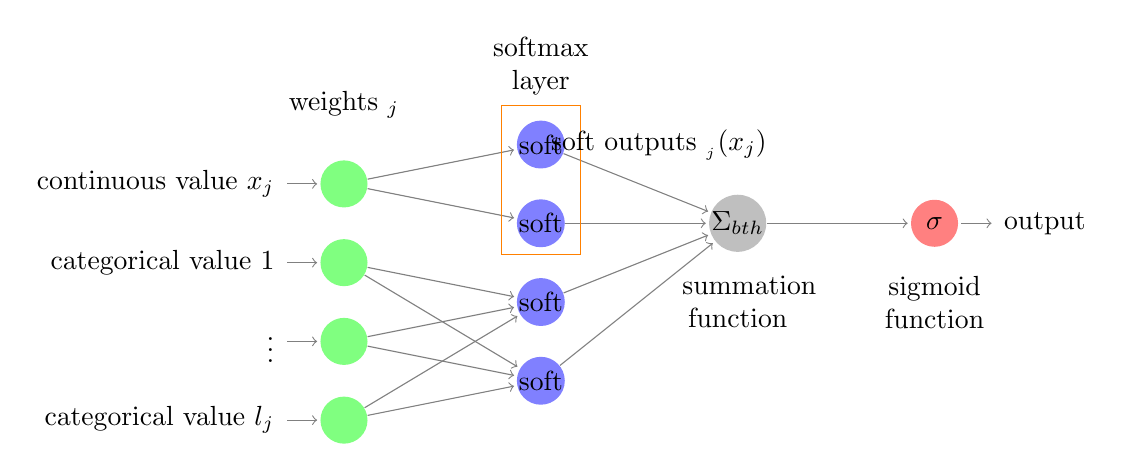
\begin{tikzpicture}[shorten >=1pt,->,draw=black!50, node distance=\layersep]
    \tikzstyle{every pin edge}=[<-,shorten <=1pt]
    \tikzstyle{neuron}=[circle,fill=black!25,minimum size=17pt,inner sep=0pt]
    \tikzstyle{input neuron}=[neuron, fill=green!50];
    \tikzstyle{output neuron}=[neuron, fill=red!50];
    \tikzstyle{hidden neuron}=[neuron, fill=blue!50];
    \tikzstyle{annot} = [text width=4em, text centered]
    \tikzstyle{annotrectangle} = [text width=8em, text centered]


        \node[input neuron, pin=left:continuous value $x_j$] (I-1) at (0,-1) {};
        
        \node[input neuron, pin=left:categorical value $1$] (I-2) at (0,-2) {};
        \node[input neuron, pin=left:$\vdots$] (I-3) at (0,-3) {};
        \node[input neuron, pin=left:categorical value $l_j$] (I-4) at (0,-4) {};

    % Draw the hidden layer nodes
    \foreach \name / \y in {1,...,2}
        \path[yshift=0.5cm]
            node[hidden neuron] (H-\name) at (\layersep,-\y cm) {soft};

    \foreach \name / \y in {3,...,4}
        \path[yshift=0.5cm]
            node[hidden neuron] (H-\name) at (\layersep,-\y cm) {soft};
            
    % Draw the sum layer node 
    
    \node[neuron, right of=H-2] (S) {$\Sigma_{\glssymbol{bth}}$};

    % Draw the output layer node
    
    \node[output neuron,pin={[pin edge={->}]right:output}, right of=S] (O) {$\sigma$};
    
    %\node[output neuron,pin={[pin edge={->}]right:Output}, right of=H-2] (O) {$\sigma(\cdot)$};
    
    

    % Connect every node in the input layer with every node in the
    % hidden layer.
%    \foreach \source in {1,...,4}
        \foreach \dest in {1,2}
            \path (I-1) edge (H-\dest);

        \foreach \dest in {3,4}
            \path (I-2) edge (H-\dest);
        \foreach \dest in {3,4}
            \path (I-3) edge (H-\dest);
        \foreach \dest in {3,4}
            \path (I-4) edge (H-\dest);

        % \foreach \dest in {5,6}
        %     \path (I-3) edge (H-\dest);

    % Connect every node in the hidden layer with the output layer
    \foreach \source in {1,...,4}
        \path (H-\source) edge (S);
        
    % connect Sigma with sigma
    \path (S) edge (O);

    % Annotate the layers
    \node[annot,above of=H-1, node distance=1cm] (hl) {softmax layer};
    \node[annot,above of=I-1,node distance=1cm] {weights $\ag_j$};
    %\node[annot,right of=hl] (s) {};
    \node[annot, below of=O, node distance=1cm] (s) {sigmoid function};
    \node[annot, below of=S,node distance=1cm] {summation function};
    
    \draw [orange] (2,0) rectangle (3,-1.9);
    % \draw [red] (2,-2) rectangle (3,-4);
    
    \node[annotrectangle,right of=H-1, node distance=1.5cm] {soft outputs $\q_{\ag_j}(x_j)$}; 

\end{tikzpicture}
\caption{Proposed shallow architecture to maximize (\ref{eq:lqa}).}
\label{fig:nn}
\end{figure}


\paragraph{Stochastic gradient descent as a quantization provider}

By relying on a stochastic gradient descent, the smoothed likelihood (\ref{eq:lqa}) can be maximized over $\left(\ag, \glssymbol{bth} \right)$. The results should be close to the maximizers of the original likelihood (\ref{eq:lq}) if the model is well-specified, when there is a true underlying quantization. In the mis-specified model case, there is no such guarantee. Therefore, to be more conservative, we evaluate at each training epoch $(t)$ the quantization $\hat{\q}^{(t)}$ resulting from the \textit{maximum a posteriori} procedure explicited in Equation~(\ref{eq:ht}), then classicaly estimate the logistic regression parameter \textit{via} maximum likelihood, as done in Equation~(\ref{eq:lq}):
\[\glssymbol{bth}^{(t)} = \argmin_{\glssymbol{bth}} \ell_{\q^{(t)}}(\glssymbol{bth}; (\glssymbol{bbx},\glssymbol{bby}))\]
and the resulting $\mbox{BIC}^{(t)}$ as in (\ref{eq:BICq}). If $T$ is a given maximum number of iterations of the stochastic gradient descent algorithm, the quantization retained at the end is then determined by the optimal epoch
\[t_*=\argmin_{t\in \{1,\ldots, T\}} \mbox{BIC}^{(t)}.\]
 
\paragraph{Choosing an appropriate number of levels}

Concerning now the number of intervals or factor levels $\boldsymbol{m} = (m_j)_1^d$, they have also to be estimated since in practice they are unknown. Looping over all candidates $\boldsymbol{m}$ is intractable. But in practice, by relying on the \textit{maximum a posteriori} procedure developed in Equation~(\ref{eq:ht}), we might drop a lot of unseen factor levels, \textit{e.g.}\ if $q_{\ag_{j,h}}(x_{i,j}) \ll 1$ for all training observations $\glssymbol{xij}$, the level $h$ ``vanishes'', \textit{i.e.}\ $\hat{q}_{j,h} = 0$. In practice, we recommend to start with a user-chosen $\bm{m}=\boldsymbol{m}_{\max}$ and we will see in the experiments of Section~\ref{sec:experiments} that the proposed approach is able to explore small values of $\boldsymbol{m}$ and to select a value $\hat{\boldsymbol{m}}$ drastically smaller than $\boldsymbol{m}_{\max}$. This phenomenon, which reduces the computational burden of the quantization task, is also illustrated in the next section.




\section{An \gls{sem} approach} \label{sec:sem}
 
 
 \textcolor{red}{reprendre article et changer notations}
 
 \textcolor{red}{penser à uniformiser caption en haut ou en bas des figures / tableaux / algorithms}

\begin{figure}
\begin{multicols}{2}
\begin{minipage}{0.45\textwidth}
\caption{\label{fig:dep}Dépendance entre $\glssymbol{X}^j$,$\E^j$ et $\glssymbol{Y}$} 
\centering
\begin{tikzpicture}
\tikzset{vertex/.style = {shape=circle,draw,minimum size=1.5em}}
\tikzset{edge/.style = {->,> = latex'}}
% vertices
\node[vertex] (x1) at  (0,1.5) {$\glssymbol{X}^1$};
\node[vertex] (xj) at  (0,0) {$\glssymbol{X}^j$};
\node[vertex] (xd) at  (0,-1.5) {$\glssymbol{X}^{d}$};

%\node[vertex] (delta) at  (2.5,3) {$\delta$};

\node[vertex] (e1) at  (2.5,1.5) {$\E^1$};
\node[vertex] (ej) at  (2.5,0) {$\E^j$};
\node[vertex] (ed) at  (2.5,-1.5) {$\E^{d}$};

\node[vertex] (y) at (5,0) {$\glssymbol{Y}$};

%edges
%\draw[edge] (x1) to (delta);
%\draw[edge] (xj) to (delta);
%\draw[edge] (xd) to (delta);

%\draw[edge] (delta) to (y);

\draw[edge] (x1) to (e1);
\draw[edge] (xj) to (ej);
\draw[edge] (xd) to (ed);
\draw[edge] (e1) to (y);
\draw[edge] (ej) to (y);
\draw[edge] (ed) to (y);

\draw[dashed] (x1) to (xj);
\draw[dashed] (xj) to (xd);

\draw[dashed] (e1) to (ej);
\draw[dashed] (ej) to (ed);
\end{tikzpicture}
\end{minipage}

\columnbreak

\begin{minipage}{0.45\textwidth}
\centering
\caption{\label{fig:disc_cont} Discrétisation d'une variable continue.}
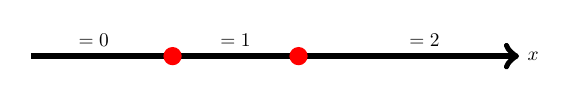
\begin{tikzpicture}[scale=0.2,every node/.style={scale=0.7}]
\draw[->,line width=0.08cm] (-5,0)--(26,0) node[right]{$\glssymbol{x}$};

\node [red,circle, fill] at (4,0) {};
\node [red,circle, fill] at (12,0) {};

\node at (-1,1) {$\E = 0$};
\node at (8,1) {$\E = 1$};
\node at (20,1) {$\E = 2$};
\end{tikzpicture}
\end{minipage}

\vfill

\begin{minipage}{0.45\textwidth}
\centering
\caption{\label{fig:disc_disc} Discrétisation d'une variable qualitative.}
\begin{tikzpicture}[scale=0.2,every node/.style={scale=0.7}]
\tikzset{vertex/.style = {shape=circle,draw,scale=0.7,minimum size=1cm}}
\tikzset{edge/.style = {->,> = latex'}}

% Boules E^j
\node [vertex] (e1) at (3,2.5) {0};
\node [vertex] (e2) at (15,2.5) {1};

% Boules X^J
\node [vertex] (x1) at (-4,0) {0};
\node [vertex] (x2) at (1.8,0) {1};
\node [vertex] (x3) at (9.5,0) {2};
\node [vertex] (x4) at (17,0) {3};
\node [vertex] (x5) at (24,0) {4};

% Labels
\node at (-7,2.5) {$\E=$};
\node at (-7,0.2) {$\glssymbol{X}=$};

% Flèches
\draw[edge,line width=0.03cm] (x1) to (e1);
\draw[edge,line width=0.03cm] (x3) to (e1);
\draw[edge,line width=0.03cm] (x4) to (e1);
\draw[edge,line width=0.03cm] (x2) to (e2);
\draw[edge,line width=0.03cm] (x5) to (e2);

\end{tikzpicture}
\end{minipage}
\end{multicols}
\end{figure}




\begin{figure}
\caption{\label{fig:exp_sim} Distribution des données simulées selon un modèle discret.}
\centering
\begin{tikzpicture}
      \draw[->] (-1,0) -- (5,0) node[right] {$x$};
      \draw[->] (0,-1) -- (0,3) node[above] {freq};
      \draw[scale=1,domain=0.5:3.5,smooth,variable=\y,red,thick]  plot ({\y},2.5);
      \draw[scale=1,domain=-1:0.5,smooth,variable=\y,red,thick]  plot ({\y},0);
      \draw[scale=1,domain=3.5:5,smooth,variable=\y,red,thick]  plot ({\y},0);
      \draw[scale=1,domain=0:2.5,smooth,variable=\x,red]  plot (0.5,{\x});
      \draw[scale=1,domain=0:2.5,smooth,variable=\x,red]  plot (3.5,{\x});
      
      \draw[scale=1,domain=-0.2:2.8,smooth,variable=\x,blue]  plot (1.5,{\x});
      \draw[scale=1,domain=-0.2:2.8,smooth,variable=\x,blue]  plot (2.5,{\x});

		\node[scale=0.7] (e1) at  (0.95,2.7) {$E=0$};
		\node[scale=0.7] (e2) at  (1.95,2.7) {$E=1$};
		\node[scale=0.7] (e3) at  (2.95,2.7) {$E=2$};

		\node[scale=0.7] (x1) at  (0.5,-0.5) {$0$};
		\node[scale=0.7] (x2) at  (1.35,-0.5) {$S_1=1/3$};
		\node[scale=0.7] (x3) at  (2.65,-0.5) {$S_2=2/3$};
		\node[scale=0.7] (x4) at  (3.5,-0.5) {$1$};

\end{tikzpicture}
\end{figure}




 
 
 \section{Numerical experiments} \label{sec:experiments}

This section is divided into three complementary parts to assess the validity of our proposal, that we call hereafter \textit{glmdisc}. First, simulated data are used to evaluate its ability to recover the true data generating mechanism. Second, the predictive quality of the new learned representation approach is illustrated on several classical benchmark datasets from the UCI library. Third, we use it on \textit{Credit Scoring} datasets provided by Credit Agricole Consumer Finance, a major European company in the consumer credit market. The Python notebooks of all experiments, excluding the confidential real data, can be found on the first author's website. \textcolor{red}{à adapter}


\subsection{Simulated data: empirical consistency and robustness}

We focus here on discretization of continuous features (similar experiments could be conducted on categorical ones). Two continuous features $x_1$ and $x_2$ are sampled from the uniform distribution on $[0,1]$ and discretized by using
\[\q_1(\cdot)=\q_2(\cdot) = (\mathds{1}_{]-\infty,1/3]}(\cdot),\mathds{1}_{]1/3,2/3]}(\cdot),\mathds{1}_{]2/3,\infty]}(\cdot)).\]
Here, following (\ref{eq:Cjhcont}), we have $d=2$ and $m_1=m_2=3$ and the cutpoints are $c_{j,1}=1/3$ and $c_{j,2}=2/3$ for $j=1,2$. Setting $\glssymbol{bth}=(0,-2,2,0,-2,2,0)$, the target feature $y$ is then sampled from $p_{\glssymbol{bth}}(\cdot | \q(\glssymbol{bbx}))$ via the logistic model (\ref{eq:reglogq}).

From the \textit{glmdisc} algorithm, we studied three cases:
\begin{enumerate}[(a)]
    \item First, the quality of the cutoff estimator $\hat{c}_{j,2}$ of $c_{j,2} = 2/3$ is assessed when the starting maximum number of intervals per discretized continuous feature is set to its true value $m_1=m_2= 3$;
    \item Second, we estimated the number of intervals $\hat{m}_1$ of $m_1=3$ when the starting maximum number of intervals per discretized continuous feature is set to $m_{\text{max}} = 10$; 
    \item Last, we added a third feature $x_3$ also drawn uniformly on $[0,1]$ but uncorrelated to $y$ and estimated the number $\hat{m}_3$ of discretization intervals selected for $x_3$. The reason is that a non-predictive feature which is discretized or grouped into a single value is \textit{de facto} excluded from the model, and this is a positive side effect.
\end{enumerate}
From a statistical point of view, experiment (a) assesses the empirical consistency of the estimation of $C_{j,h}$, whereas experiments (b) and (c) focus on the consistency of the estimation of $m_j$. The results are summarized in Table~\ref{tab:estim_precision} where 95\% confidence intervals (CI) are given, with a varying sample size. Note in particular that the slight underestimation in (b) is a classical consequence of the BIC criterion on small samples. 
\begin{table}[h!]
    \centering
\begin{tabular}{llll}
Sample size & (a) $\hat{c}_{j,2}$ & (b) $\hat{m}_1$ & (c) $\hat{m}_3$\\
\hline
\hline
\multicolumn{4}{c}{\textit{glmdisc}-NN} \\
\hline
$n = 1,000$ & $[0.656,0.666]$ & $[2.679,2.941]$ & $[1.326,1.554]$ \\
$n = 10,000$ & $[0.666,0.666]$ & $[3.000,3.000]$ & $[1.399,1.621]$ \\
\hline
\multicolumn{4}{c}{\textit{glmdisc}-SEM} \\
\hline
$n = 1,000$ & $[0]$ & $[2]$ & $[1]$ \\
$n = 10,000$ & $[0]$ & $[3]$ & $[1]$ 
\end{tabular}
    \caption{(a) CI of $\hat{c}_{j,2}$ for $c_{j,2} = 2/3$. (b) CI of $\hat{m}$ for $m_1=3$. (c) CI of $\hat{m}_3$ for $m_3=1$.}
    \label{tab:estim_precision}
\end{table}

 \newlength\figureheight
 \newlength\figurewidth
 \setlength\figureheight{4cm}
 \setlength\figurewidth{14cm}
 
  \begin{figure}
    \centering
    \begin{subfigure}[t]{\textwidth}
        \centering
        % This file was created by matplotlib2tikz v0.6.18.
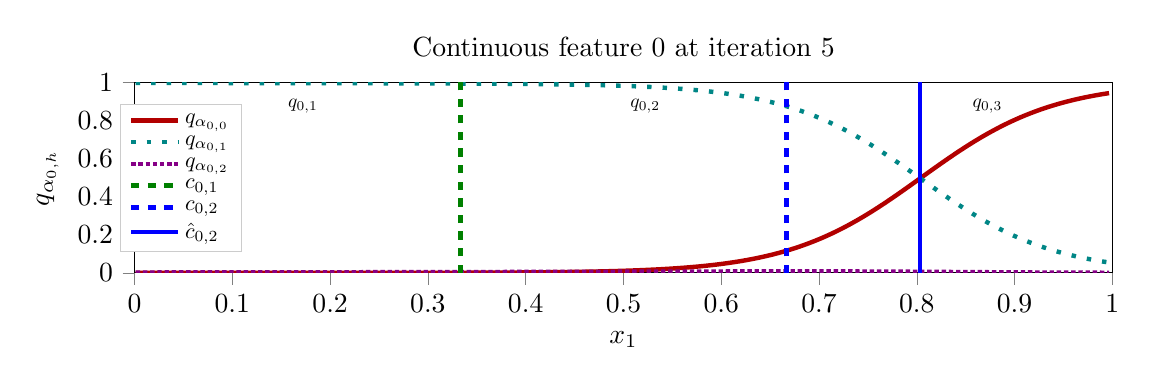
\begin{tikzpicture}

\definecolor{color0}{rgb}{0,0.75,0.75}
\definecolor{color1}{rgb}{0.75,0,0.75}

\begin{axis}[
height=\figureheight,
legend cell align={left},
legend entries={{${q}_{\bm{\alpha}_{0,0}}$},{${q}_{\bm{\alpha}_{0,1}}$},{${q}_{\bm{\alpha}_{0,2}}$},{$c_{0,1}$},{$c_{0,2}$},{$\hat{c}_{0,2}$}},
legend style={at={(0.11,0.5)}, anchor=east, draw=white!80.0!black, nodes={scale=0.8, transform shape}},
tick align=outside,
tick pos=left,
title={Continuous feature 0 at iteration 5},
width=\figurewidth,
x grid style={white!69.01960784313725!black},
xlabel={$x_1$},
xmin=0, xmax=1,
y grid style={white!69.01960784313725!black},
ylabel={${q}_{\bm{\alpha}_{0,h}}$},
ymin=0, ymax=1
]
\addlegendimage{no markers, ultra thick, red!70.0!black}
\addlegendimage{no markers, ultra thick, loosely dotted, color0!70.0!black}
\addlegendimage{no markers, ultra thick, densely dotted, color1!70.0!black}
\addlegendimage{no markers, ultra thick, dashed, green!50.0!black}
\addlegendimage{no markers, ultra thick, dashed, blue}
\addlegendimage{no markers, ultra thick, blue}
\addplot [ultra thick, red!70.0!black]
table [row sep=\\]{%
0.00121733135182733	7.28208306099987e-06 \\
0.00399800202767708	7.58670148570673e-06 \\
0.00428590830880138	7.61897081247298e-06 \\
0.00583511703754613	7.79491892899387e-06 \\
0.00722810751864345	7.95659889263334e-06 \\
0.00883092408680852	8.14678696769988e-06 \\
0.00892196292255498	8.15773091744632e-06 \\
0.0091566517099908	8.18599528429331e-06 \\
0.00923090984674624	8.19496017356869e-06 \\
0.0100966686316811	8.30019325803732e-06 \\
0.0121625222007031	8.55678172229091e-06 \\
0.0145607215360531	8.86461384652648e-06 \\
0.0148124296089015	8.89756756805582e-06 \\
0.0155108668507814	8.98961661732756e-06 \\
0.016388930761377	9.1067049652338e-06 \\
0.0165505671244613	9.12842642719625e-06 \\
0.0171573414191398	9.21042283152929e-06 \\
0.0193168803366051	9.5082732514129e-06 \\
0.0196176080342491	9.55050745687913e-06 \\
0.0199828289521065	9.60205215960741e-06 \\
0.0217553532903839	9.85618589766091e-06 \\
0.0218823859122642	9.87465773505392e-06 \\
0.0228894296421823	1.00222969194874e-05 \\
0.0231678236934525	1.00635033959406e-05 \\
0.0234639524336395	1.01075220300118e-05 \\
0.0240819943997985	1.02000030892668e-05 \\
0.0245627106801373	1.0272529834765e-05 \\
0.0245889454935851	1.02765061456012e-05 \\
0.0254639162068063	1.04098771771532e-05 \\
0.0259388906266036	1.04829960037023e-05 \\
0.0263836623637999	1.05519393400755e-05 \\
0.0270972950820486	1.0663491593732e-05 \\
0.0283300913612849	1.08590038507828e-05 \\
0.0286622934193979	1.0912292964349e-05 \\
0.0298828118815666	1.11103545350488e-05 \\
0.0300746747069074	1.11418121377937e-05 \\
0.0311555148727282	1.13207161120954e-05 \\
0.0317077923073903	1.14132371891174e-05 \\
0.0332701482181197	1.16790743049933e-05 \\
0.0342621296009059	1.18510679385508e-05 \\
0.0343279985540969	1.18625748655177e-05 \\
0.0344243967448893	1.18794378067832e-05 \\
0.0345313526152026	1.18981834020815e-05 \\
0.0348501916637685	1.19542119136895e-05 \\
0.0349907508243421	1.19790020107757e-05 \\
0.0359872504585017	1.21562261483632e-05 \\
0.0362310024928287	1.21999692055397e-05 \\
0.0366095524509532	1.22682231449289e-05 \\
0.0379176486074634	1.25070264402893e-05 \\
0.0403385868224699	1.29613108583726e-05 \\
0.0409980934669582	1.30878970594495e-05 \\
0.0411009563963477	1.31077504192945e-05 \\
0.0416433618426197	1.32129607663956e-05 \\
0.0434312735145819	1.3565721019404e-05 \\
0.0441433900213135	1.37088472911273e-05 \\
0.0453507593315232	1.39549465529853e-05 \\
0.0465425722547385	1.42022299769451e-05 \\
0.048055790853058	1.4522497622238e-05 \\
0.0498244429652048	1.4905996977177e-05 \\
0.0499138395223641	1.49256620716187e-05 \\
0.0500224768452724	1.49495708683389e-05 \\
0.0501451025944044	1.4976602869865e-05 \\
0.0508313343201909	1.51288422785001e-05 \\
0.0528287617134601	1.55807992996415e-05 \\
0.0554318613335167	1.61901243700413e-05 \\
0.0568944168268039	1.6542880985071e-05 \\
0.0580421671310021	1.6825060811243e-05 \\
0.0581829367774224	1.68600145116216e-05 \\
0.0582464981538736	1.68758051586337e-05 \\
0.061138324915142	1.76105386344716e-05 \\
0.0661100314140015	1.89492729987251e-05 \\
0.0666057899124018	1.90882237802725e-05 \\
0.0669707761967708	1.91911694855662e-05 \\
0.0671266686577333	1.92353090824327e-05 \\
0.0686662733539142	1.96767341549275e-05 \\
0.0692515177638677	1.98471716430504e-05 \\
0.0700522852791065	2.00827926164493e-05 \\
0.0708166409087652	2.03102663363097e-05 \\
0.0739831283273903	2.12805007322459e-05 \\
0.0744557758040519	2.14292322198162e-05 \\
0.0760071681977798	2.19248086068546e-05 \\
0.076598016264572	2.21165482798824e-05 \\
0.0770973657055851	2.2279889890342e-05 \\
0.0783565293465318	2.26971715164836e-05 \\
0.078406381150142	2.27138589252718e-05 \\
0.0784226663514104	2.2719314074493e-05 \\
0.0801910475982274	2.33191640290897e-05 \\
0.0811497869224936	2.36509677051799e-05 \\
0.0820428097289791	2.39642740780255e-05 \\
0.0824186797205529	2.40973931795452e-05 \\
0.0842277962246097	2.47484822466504e-05 \\
0.0860509183129933	2.54223905358231e-05 \\
0.0871811255235175	2.58493655564962e-05 \\
0.0878315304280046	2.60983015323291e-05 \\
0.0887988354863684	2.64730060735019e-05 \\
0.0897338519259113	2.68402909568977e-05 \\
0.0899271697891475	2.69168558588717e-05 \\
0.0919787717665748	2.77430881396867e-05 \\
0.0935526652379582	2.83940808003535e-05 \\
0.0939090065052064	2.85435580735793e-05 \\
0.0945988870347061	2.88352257484803e-05 \\
0.096618912882444	2.97065198537894e-05 \\
0.0970084891114591	2.98775448754895e-05 \\
0.0984122603995672	3.05020203086315e-05 \\
0.100207604620953	3.13197815557942e-05 \\
0.100212527088041	3.1322048016591e-05 \\
0.100799383077452	3.15940960717853e-05 \\
0.102777212518229	3.25285145663656e-05 \\
0.10355794511468	3.29049144056626e-05 \\
0.103777986851009	3.30117654812057e-05 \\
0.104283245534613	3.32584895659238e-05 \\
0.104926828677962	3.35754084517248e-05 \\
0.105048147684541	3.3635507861618e-05 \\
0.105888629613813	3.40546612278558e-05 \\
0.106594265398706	3.44106410921086e-05 \\
0.107659824617846	3.49552283296362e-05 \\
0.108236845622617	3.52537172148004e-05 \\
0.108525705010578	3.54041185346432e-05 \\
0.110299453724928	3.63417166227009e-05 \\
0.1109411277088	3.66869680874515e-05 \\
0.114327603236688	3.85642633773386e-05 \\
0.114459519996847	3.86392894142773e-05 \\
0.117867979538534	4.06296021537855e-05 \\
0.118112325438648	4.0776143578114e-05 \\
0.118633260119092	4.10903630836401e-05 \\
0.11982692170167	4.18194977100939e-05 \\
0.120297266407184	4.21103977714665e-05 \\
0.12058353024893	4.22883931605611e-05 \\
0.120831487175604	4.24431891588029e-05 \\
0.12100766940383	4.25535436079372e-05 \\
0.121149329304323	4.26424703618977e-05 \\
0.12132073351728	4.27503218816128e-05 \\
0.124248653311104	4.4635158701567e-05 \\
0.126006965902748	4.58067588624544e-05 \\
0.126901124475677	4.64143231511116e-05 \\
0.126954279439678	4.64506993012037e-05 \\
0.128893135931382	4.77969442727044e-05 \\
0.129130414500304	4.79643531434704e-05 \\
0.129265754179532	4.80601411254611e-05 \\
0.129318382573767	4.80974013044033e-05 \\
0.12957327546953	4.82783798361197e-05 \\
0.129620549409663	4.83120311400853e-05 \\
0.130028516874333	4.86033604829572e-05 \\
0.131097613537266	4.93751103931572e-05 \\
0.133250294991105	5.09664569108281e-05 \\
0.13328775473883	5.09945930389222e-05 \\
0.13407228993995	5.15875399287324e-05 \\
0.134949207751391	5.22584632562939e-05 \\
0.138173080751483	5.48009811609518e-05 \\
0.138829427196237	5.53335412405431e-05 \\
0.13934817040543	5.575812610914e-05 \\
0.140500928037371	5.67133829463273e-05 \\
0.141075328307274	5.71954187762458e-05 \\
0.142185810887561	5.8139041357208e-05 \\
0.143422034202274	5.92078358749859e-05 \\
0.143493165626466	5.92698961554561e-05 \\
0.144195876538432	5.98867954977322e-05 \\
0.148766937684016	6.40595244476572e-05 \\
0.150763038004328	6.59716606605798e-05 \\
0.151522077107299	6.67136700940318e-05 \\
0.152255804124635	6.74388211336918e-05 \\
0.15226616541564	6.74491093377583e-05 \\
0.153023332064105	6.82059180689976e-05 \\
0.153075622362746	6.82584723108448e-05 \\
0.153205273538633	6.83889811625704e-05 \\
0.155085023545417	7.03097248333506e-05 \\
0.15772483711392	7.3098526627291e-05 \\
0.158186389101905	7.35973080736585e-05 \\
0.15894693490281	7.4426774517633e-05 \\
0.159639800043974	7.51905172364786e-05 \\
0.160146141938642	7.57535599404946e-05 \\
0.160729957792949	7.64081050874665e-05 \\
0.160844366590924	7.65369841246866e-05 \\
0.16282671011704	7.88055913290009e-05 \\
0.163830519374535	7.99798726802692e-05 \\
0.163992249762284	8.01706846687011e-05 \\
0.164417055397194	8.0674079072196e-05 \\
0.165260696441198	8.16832107375376e-05 \\
0.167361304418963	8.42509107314982e-05 \\
0.169491743858274	8.6937659943942e-05 \\
0.170198366879178	8.78475184435956e-05 \\
0.17056212452737	8.83196917129681e-05 \\
0.170912119394526	8.87762944330461e-05 \\
0.172648789750251	9.1077308752574e-05 \\
0.172856178369217	9.1356057964731e-05 \\
0.173162955842619	9.17699871934019e-05 \\
0.173717258172562	9.25224885577336e-05 \\
0.174916773476619	9.4172362878453e-05 \\
0.175269110850529	9.46624713833444e-05 \\
0.175796530948979	9.54010392888449e-05 \\
0.176965388380551	9.70582841546275e-05 \\
0.177321345888588	9.75686998572201e-05 \\
0.177435150590059	9.77323215920478e-05 \\
0.178853029237583	9.97956958599389e-05 \\
0.179003818378901	0.000100017561635468 \\
0.180108329801849	0.000101658624771517 \\
0.18098127250095	0.000102974656329025 \\
0.181164449059833	0.000103252881672233 \\
0.181504936132438	0.000103772319562268 \\
0.181698184610282	0.000104068181826733 \\
0.181706779152786	0.000104081373137888 \\
0.183508352968371	0.00010688114707591 \\
0.18371338802759	0.000107204468804412 \\
0.184634680521775	0.000108669708424713 \\
0.18715264530893	0.00011277695739409 \\
0.187902267731003	0.000114029448013753 \\
0.188039517539109	0.000114260292320978 \\
0.18935042046278	0.000116488750791177 \\
0.190047732419662	0.000117691670311615 \\
0.190622119303773	0.000118691881652921 \\
0.191971593527005	0.000121075514471158 \\
0.193283500603906	0.000123438512673602 \\
0.197644387198593	0.000131630062242039 \\
0.19852231723701	0.000133343666675501 \\
0.200336272290021	0.000136955481139012 \\
0.200653415987652	0.000137596958666109 \\
0.20282835566531	0.000142077537020668 \\
0.205443999059423	0.000147659637150355 \\
0.207292923022167	0.000151737200212665 \\
0.208117425413999	0.000153591696289368 \\
0.210007644411429	0.000157929171109572 \\
0.213557102615423	0.000166407713550143 \\
0.215277579547195	0.000170679515576921 \\
0.215497345364033	0.000171232954016887 \\
0.216310718872085	0.00017329741967842 \\
0.216355091614949	0.000173410589923151 \\
0.217392921106891	0.000176082437974401 \\
0.217574656587144	0.000176554473000579 \\
0.22044293838767	0.000184174932655878 \\
0.220716468008851	0.000184918695595115 \\
0.222115983638242	0.000188770980457775 \\
0.222246464423612	0.000189134341781028 \\
0.22273747409856	0.0001905073877424 \\
0.224665735391259	0.00019599670486059 \\
0.226091799609793	0.000200158072402701 \\
0.226553200069555	0.000201523129362613 \\
0.227270480715813	0.000203664050786756 \\
0.227447153120765	0.00020419477368705 \\
0.227729308234277	0.000205045376787893 \\
0.228445973454936	0.000207221732125618 \\
0.230001408006134	0.000212024853681214 \\
0.230452444453415	0.000213438281207345 \\
0.23101774976842	0.000215223204577342 \\
0.232175303582309	0.000218924949876964 \\
0.238608988543593	0.000240689216298051 \\
0.238816890215772	0.000241427536820993 \\
0.241051513831921	0.000249507313128561 \\
0.24158011969787	0.000251457880949602 \\
0.241902400534758	0.000252654514042661 \\
0.245972048559771	0.000268264237092808 \\
0.246055548554611	0.000268594478257 \\
0.246667080102265	0.00027102482272312 \\
0.249063142333596	0.000280761771136895 \\
0.2492389743227	0.000281489861663431 \\
0.250289311607262	0.00028587892302312 \\
0.250515586119678	0.000286833412246779 \\
0.250940657287891	0.000288635026663542 \\
0.25167183440657	0.00029176048701629 \\
0.257990385058828	0.000320219376590103 \\
0.258124141751891	0.000320850958814844 \\
0.258177043220415	0.000321100844303146 \\
0.259695612003727	0.000328364403685555 \\
0.259776131366315	0.000328754162183031 \\
0.260071715391803	0.000330188486259431 \\
0.261863459876915	0.000339018617523834 \\
0.262327493161023	0.000341343693435192 \\
0.26759593699964	0.000368886889191344 \\
0.268489073403659	0.00037377150147222 \\
0.268717231393198	0.000375029660062864 \\
0.268959947078319	0.000376372714526951 \\
0.270587931966637	0.000385506573366001 \\
0.270690946459964	0.000386091909604147 \\
0.271962599626952	0.000393391470424831 \\
0.272078011383322	0.000394060742110014 \\
0.273472308124372	0.000402236852096394 \\
0.2748160216297	0.000410276494221762 \\
0.27486022346705	0.000410543754696846 \\
0.276792319224663	0.000422394019551575 \\
0.277649825865711	0.000427762279286981 \\
0.278253018986364	0.000431579304859042 \\
0.278408961673642	0.000432571803685278 \\
0.280420535697693	0.000445578916696832 \\
0.280986539769637	0.000449308601673692 \\
0.282010151037797	0.000456133158877492 \\
0.282040248224806	0.000456335488706827 \\
0.282123909223068	0.000456898211268708 \\
0.285513331048722	0.000480283721117303 \\
0.287573265929611	0.00049507716903463 \\
0.288706085955357	0.00050340557936579 \\
0.290405917039397	0.000516166153829545 \\
0.290997388676799	0.000520681671332568 \\
0.291345467206721	0.000523357535712421 \\
0.291398859476294	0.000523769005667418 \\
0.291913353201399	0.000527752446942031 \\
0.292457883757979	0.000532001198735088 \\
0.293034823854815	0.000536540756002069 \\
0.293967194785546	0.00054395804181695 \\
0.294530422037374	0.000548488169442862 \\
0.294989677655505	0.000552210316527635 \\
0.297159059538413	0.000570135714951903 \\
0.297297208003757	0.000571296841371804 \\
0.297401117461309	0.000572171877138317 \\
0.297596325223743	0.000573818746488541 \\
0.297864053288129	0.000576085294596851 \\
0.30177729109265	0.00061025598552078 \\
0.303412381953207	0.000625127053353935 \\
0.303804315308251	0.000628744601272047 \\
0.304062576428461	0.000631140486802906 \\
0.305272733951204	0.000642487313598394 \\
0.308571936874729	0.000674467766657472 \\
0.308642296164111	0.000675167189911008 \\
0.308753468839242	0.000676273077260703 \\
0.313549155412623	0.00072574958903715 \\
0.313653278508487	0.000726862985175103 \\
0.314321905263844	0.000734053726773709 \\
0.315143369330536	0.000742985575925559 \\
0.315610968893992	0.000748117978218943 \\
0.315614001089602	0.000748151389416307 \\
0.316213538079681	0.000754784152377397 \\
0.31656704193251	0.000758722890168428 \\
0.317033096183104	0.000763946096412838 \\
0.318077975465148	0.000775788968894631 \\
0.318499630211901	0.000780619448050857 \\
0.320459324952121	0.000803468690719455 \\
0.321158026386313	0.000811775680631399 \\
0.324068371830885	0.000847310700919479 \\
0.325719114944994	0.00086815282702446 \\
0.32726449148383	0.000888128124643117 \\
0.327515376124492	0.000891414179932326 \\
0.328913020135104	0.000909943948499858 \\
0.329471410393436	0.000917453726287931 \\
0.329483556970732	0.00091761804651469 \\
0.329807282212852	0.000922000617720187 \\
0.330833599133424	0.000936035183258355 \\
0.33305761718435	0.000967183266766369 \\
0.334466305551428	0.000987446634098887 \\
0.336209591213773	0.00101311039179564 \\
0.339174876956243	0.00105830410029739 \\
0.339882470276715	0.00106938323006034 \\
0.34038186985453	0.00107727176509798 \\
0.341801626815983	0.00110001757275313 \\
0.343524436417214	0.00112826353870332 \\
0.343689611464564	0.00113101024180651 \\
0.344781691139359	0.00114933389704674 \\
0.345591136214371	0.0011631048982963 \\
0.346919336340971	0.00118606234900653 \\
0.347671848387079	0.00119926850311458 \\
0.348163376208385	0.00120797427371144 \\
0.349472519093074	0.00123147061094642 \\
0.349745522231846	0.00123642687685788 \\
0.351374549797252	0.00126642279792577 \\
0.35188450877064	0.00127596128731966 \\
0.356410987959693	0.00136383273638785 \\
0.357063359912744	0.00137698603793979 \\
0.35766224198294	0.00138917204458266 \\
0.359634636963466	0.00143007305450737 \\
0.359702418340943	0.00143149995710701 \\
0.360059525411196	0.00143904110882431 \\
0.360289892612103	0.00144392531365156 \\
0.360991066472348	0.00145889667328447 \\
0.361517661936521	0.00147024297621101 \\
0.362811795477131	0.00149850116576999 \\
0.363672312199373	0.00151758955325931 \\
0.364539422226955	0.00153706991113722 \\
0.364777329717716	0.00154245877638459 \\
0.366260111813999	0.00157647219020873 \\
0.366299975782456	0.0015773962950334 \\
0.366824068875263	0.00158960372209549 \\
0.366852341843951	0.00159026484470814 \\
0.367255430778636	0.00159972032997757 \\
0.367718612255156	0.00161065638530999 \\
0.371844893263566	0.00171143340412527 \\
0.373914699139864	0.00176432984881103 \\
0.375334232083758	0.001801548874937 \\
0.375994866909118	0.00181913608685136 \\
0.376668338720068	0.0018372421618551 \\
0.377076405033397	0.00184830033686012 \\
0.377984484345733	0.00187314569484442 \\
0.378411364752534	0.00188494066242129 \\
0.378781645976558	0.00189523107837886 \\
0.378969500633152	0.00190047372598201 \\
0.380503918700316	0.00194384052883834 \\
0.382290922993942	0.00199559051543474 \\
0.382702553179553	0.00200770422816277 \\
0.384322573332172	0.00205609761178493 \\
0.385259749331941	0.00208462332375348 \\
0.387372760421529	0.00215039239265025 \\
0.387555538130506	0.00215617823414505 \\
0.38907064039843	0.00220473832450807 \\
0.389579566720786	0.00222129351459444 \\
0.389767492364477	0.00222743907943368 \\
0.392492189498792	0.00231845513917506 \\
0.393836249332015	0.00236471043899655 \\
0.395499606909982	0.00242322916164994 \\
0.395882251973212	0.00243689399212599 \\
0.396415701753994	0.00245607364922762 \\
0.396441121576172	0.00245699170045555 \\
0.396574304024945	0.00246180547401309 \\
0.397759074483525	0.00250504142604768 \\
0.39792914466779	0.00251130945980549 \\
0.39903214396726	0.00255234399810433 \\
0.399785344239434	0.00258074980229139 \\
0.400492759495042	0.00260771438479424 \\
0.401432469526815	0.00264396821148694 \\
0.401683506422962	0.00265373918227851 \\
0.403117526972048	0.00271024508401752 \\
0.403655328822729	0.00273174326866865 \\
0.404677310156115	0.00277306651696563 \\
0.404776114127771	0.00277709611691535 \\
0.409382548454498	0.00297150947153568 \\
0.409383683968994	0.00297155906446278 \\
0.411266446539173	0.00305487471632659 \\
0.413513881114749	0.0031573842279613 \\
0.415418916892999	0.00324695720337331 \\
0.415684791078115	0.00325965881347656 \\
0.415897400040632	0.00326984981074929 \\
0.416751124277095	0.00331109552644193 \\
0.420526451622837	0.00349979870952666 \\
0.421389674091991	0.00354442722164094 \\
0.422435717298333	0.00359927117824554 \\
0.425131879618846	0.00374455796554685 \\
0.426344701070752	0.00381180131807923 \\
0.42646767360874	0.00381868635304272 \\
0.426723043204646	0.00383302103728056 \\
0.427177869701464	0.0038586906157434 \\
0.427843332102008	0.00389655632898211 \\
0.430519905858631	0.00405262690037489 \\
0.431329847429739	0.00410106917843223 \\
0.43280912191732	0.00419103866443038 \\
0.435328420042426	0.0043488098308444 \\
0.437335390870841	0.00447871256619692 \\
0.438093952949238	0.00452880887314677 \\
0.438539868644415	0.0045585217885673 \\
0.438622154375097	0.00456402543932199 \\
0.440101706010519	0.00466412073001266 \\
0.441692841095718	0.00477420352399349 \\
0.442760304995134	0.00484950467944145 \\
0.443866566189192	0.00492878723889589 \\
0.445656815071723	0.00505982572212815 \\
0.446306999832311	0.00510827312245965 \\
0.446539778293263	0.00512572936713696 \\
0.447015636734589	0.00516160065308213 \\
0.447764619143311	0.00521855987608433 \\
0.450701475867445	0.0054480223916471 \\
0.451256246885538	0.00549248280003667 \\
0.452657062023863	0.00560635421425104 \\
0.453713810202396	0.005693803075701 \\
0.455679938271804	0.00586013961583376 \\
0.458387666537298	0.00609714584425092 \\
0.458683449593184	0.00612360611557961 \\
0.458715521584147	0.00612648250535131 \\
0.461316576778666	0.00636424357071519 \\
0.461325542738979	0.00636508176103234 \\
0.463543573073144	0.0065750852227211 \\
0.465979585607885	0.00681366492062807 \\
0.467407797462426	0.00695751840248704 \\
0.468691827800416	0.00708942161872983 \\
0.468898574730863	0.00711088720709085 \\
0.472124347134469	0.00745434314012527 \\
0.473167350177021	0.0075688804499805 \\
0.475892207786094	0.00787641108036041 \\
0.476447833983088	0.00794062111526728 \\
0.476852808050028	0.00798775069415569 \\
0.480153820674186	0.0083824060857296 \\
0.481331481462533	0.00852782465517521 \\
0.481907398972557	0.00859985407441854 \\
0.482340193954975	0.00865437649190426 \\
0.483064633983067	0.00874640699476004 \\
0.484404961256947	0.00891923997551203 \\
0.484965300777859	0.00899249780923128 \\
0.486726527314222	0.0092266583815217 \\
0.487116327031527	0.00927929021418095 \\
0.488921795423616	0.0095269875600934 \\
0.489759269088015	0.00964409206062555 \\
0.490909081458542	0.00980720389634371 \\
0.49091604463621	0.00980820134282112 \\
0.492300495791636	0.0100082447752357 \\
0.4923307300145	0.0100126583129168 \\
0.492381040900871	0.0100200036540627 \\
0.49359088600479	0.010198331438005 \\
0.493621516312431	0.0102028828114271 \\
0.494440937544777	0.0103254951536655 \\
0.494453842969403	0.0103274388238788 \\
0.495146776944368	0.0104322740808129 \\
0.495982811187486	0.0105601726099849 \\
0.497062669506957	0.010727665387094 \\
0.497330994039467	0.0107696894556284 \\
0.498153946067205	0.0108995977789164 \\
0.498455749672111	0.0109476270154119 \\
0.498730582702143	0.0109915398061275 \\
0.499638616573585	0.0111378887668252 \\
0.500015331367196	0.0111991614103317 \\
0.501350798827707	0.0114191016182303 \\
0.501744525678089	0.0114847458899021 \\
0.5036535166819	0.0118083953857422 \\
0.504487562746051	0.0119526078924537 \\
0.508463499372222	0.0126643385738134 \\
0.509687293635359	0.0128917153924704 \\
0.509914323813028	0.0129343438893557 \\
0.511341386088067	0.0132054574787617 \\
0.512018604529405	0.0133360773324966 \\
0.513861444023579	0.0136979762464762 \\
0.514960109685398	0.0139183355495334 \\
0.515737002786438	0.0140762524679303 \\
0.519058118042992	0.0147714940831065 \\
0.519916366374704	0.0149565991014242 \\
0.521499066868756	0.0153039451688528 \\
0.52201095621904	0.0154179893434048 \\
0.524040740980263	0.0158784482628107 \\
0.524478728901278	0.0159795712679625 \\
0.525423938335719	0.016199953854084 \\
0.525635126495304	0.0162495970726013 \\
0.52719728420485	0.0166215300559998 \\
0.52996761968302	0.0173017662018538 \\
0.530301937454978	0.0173856746405363 \\
0.531840017863588	0.0177769474685192 \\
0.531981886047464	0.0178134646266699 \\
0.532012239031215	0.0178212765604258 \\
0.533028472048003	0.0180851742625237 \\
0.533892144890962	0.0183124449104071 \\
0.537533560414064	0.0193019192665815 \\
0.537969095533598	0.0194237008690834 \\
0.538335797788309	0.0195268373936415 \\
0.539116247263892	0.019748130813241 \\
0.542861601060095	0.0208447184413671 \\
0.54363288334093	0.0210778303444386 \\
0.543801322498743	0.0211290810257196 \\
0.547002474800456	0.0221265275031328 \\
0.548908529730498	0.0227421391755342 \\
0.550793838508607	0.0233674962073565 \\
0.553233155778543	0.0242015533149242 \\
0.554063975822177	0.0244922060519457 \\
0.554664151973859	0.0247042700648308 \\
0.555237937942708	0.0249087177217007 \\
0.556147032749051	0.0252359826117754 \\
0.556971759420448	0.0255364999175072 \\
0.557200406957364	0.0256204288452864 \\
0.557472354513669	0.025720588862896 \\
0.557634255107793	0.0257803983986378 \\
0.557665270553959	0.0257919002324343 \\
0.558053776980733	0.0259360615164042 \\
0.559718195298125	0.0265625696629286 \\
0.560469384381131	0.026850126683712 \\
0.561223854392744	0.0271419826894999 \\
0.561301666038306	0.0271722599864006 \\
0.561798210581049	0.0273662377148867 \\
0.562009451463098	0.0274491757154465 \\
0.562833608522221	0.027775052934885 \\
0.564513388059411	0.028450945392251 \\
0.566269134382303	0.0291744638234377 \\
0.567354059069172	0.0296304374933243 \\
0.567568119614931	0.0297212097793818 \\
0.568027250200944	0.0299168098717928 \\
0.568168895571326	0.0299774017184973 \\
0.568859714229155	0.0302746687084436 \\
0.569040001476579	0.0303527116775513 \\
0.569210703701173	0.0304268095642328 \\
0.56954243172626	0.0305712465196848 \\
0.570337723054723	0.0309202820062637 \\
0.570715244097907	0.0310873240232468 \\
0.57424855250552	0.0326934829354286 \\
0.575002703666514	0.033046580851078 \\
0.575003549718568	0.0330469571053982 \\
0.575679471524471	0.0333665162324905 \\
0.575807053629817	0.0334271751344204 \\
0.576466959777726	0.0337426029145718 \\
0.576872834170159	0.0339380167424679 \\
0.579766556433004	0.0353633165359497 \\
0.580763685611283	0.0358676761388779 \\
0.581439442781873	0.0362134128808975 \\
0.582738039976926	0.0368868373334408 \\
0.583406899826349	0.037238385528326 \\
0.583621843838165	0.0373520217835903 \\
0.584022416391563	0.0375646837055683 \\
0.584157343282694	0.0376365929841995 \\
0.584398535047123	0.0377654582262039 \\
0.588037407975546	0.0397618114948273 \\
0.591515761019391	0.0417643561959267 \\
0.59169858018679	0.0418722108006477 \\
0.591779783399284	0.0419201962649822 \\
0.593283454206354	0.0428186394274235 \\
0.593390679676707	0.0428834185004234 \\
0.593962031860602	0.0432300418615341 \\
0.594200655435401	0.0433756373822689 \\
0.596969362786692	0.0450993403792381 \\
0.598437319346411	0.0460394881665707 \\
0.599474715240117	0.0467151179909706 \\
0.602362270570747	0.0486457087099552 \\
0.603334150143409	0.049312312155962 \\
0.603632921169445	0.049519021064043 \\
0.60379362440282	0.0496305078268051 \\
0.604659766964252	0.0502355843782425 \\
0.605395322349658	0.0507548935711384 \\
0.606463918589886	0.051518402993679 \\
0.606775419688025	0.0517430119216442 \\
0.607357857377935	0.0521655008196831 \\
0.607580561722253	0.0523278824985027 \\
0.608621286245357	0.0530931279063225 \\
0.609575970841381	0.053804375231266 \\
0.610347066222159	0.0543853677809238 \\
0.612177604245754	0.0557883866131306 \\
0.613326929015952	0.0566866509616375 \\
0.614270777301711	0.0574344918131828 \\
0.614798584840558	0.057856660336256 \\
0.616647348049137	0.059358611702919 \\
0.616860752444383	0.0595342963933945 \\
0.617045516373702	0.059686828404665 \\
0.618083376848042	0.0605503544211388 \\
0.621554333086694	0.0635239034891129 \\
0.623029526806788	0.064828485250473 \\
0.624069668412363	0.0657632872462273 \\
0.624143156449471	0.0658297836780548 \\
0.625318868337709	0.0669025033712387 \\
0.627896177690147	0.0693109780550003 \\
0.62805232111942	0.069459356367588 \\
0.629405663035747	0.0707585513591766 \\
0.629846029847146	0.0711860731244087 \\
0.630467114324592	0.0717931464314461 \\
0.630546820907001	0.0718713775277138 \\
0.631083637650338	0.0724005177617073 \\
0.631324147788059	0.0726386830210686 \\
0.632680726177628	0.0739958137273788 \\
0.632823775680698	0.0741402879357338 \\
0.633074796432523	0.0743944495916367 \\
0.636612707474017	0.0780621990561485 \\
0.639030758002587	0.0806633904576302 \\
0.640237995740933	0.0819915160536766 \\
0.640853111920735	0.0826758369803429 \\
0.640965174455041	0.0828010365366936 \\
0.641077861086201	0.0829271748661995 \\
0.641318662912942	0.0831972286105156 \\
0.642222835181407	0.084218330681324 \\
0.64234387506577	0.084355890750885 \\
0.643801671660635	0.0860287845134735 \\
0.644160446263096	0.086445078253746 \\
0.645423350530499	0.087924912571907 \\
0.646045259468861	0.0886620879173279 \\
0.646175373815422	0.0888169780373573 \\
0.646229368496451	0.0888813659548759 \\
0.64633540284767	0.0890079215168953 \\
0.647248616680538	0.0901042148470879 \\
0.647279370177658	0.0901413559913635 \\
0.648437609650589	0.0915499180555344 \\
0.648804842952185	0.0920005887746811 \\
0.650925300722929	0.0946421846747398 \\
0.651147043039429	0.0949224084615707 \\
0.651662018637987	0.0955757722258568 \\
0.651706157147625	0.0956320092082024 \\
0.654010541995451	0.0986069887876511 \\
0.654559822635481	0.0993283167481422 \\
0.655118993248004	0.100067250430584 \\
0.655470347269005	0.10053413361311 \\
0.656959015265393	0.102533556520939 \\
0.657756536283002	0.103619195520878 \\
0.65779828590582	0.103676319122314 \\
0.657827620225886	0.103716500103474 \\
0.657888612459039	0.103799976408482 \\
0.659397129207233	0.105884462594986 \\
0.660938309454123	0.108052082359791 \\
0.661236182036626	0.108475491404533 \\
0.661269452289108	0.108522847294807 \\
0.662216186165834	0.109878912568092 \\
0.662950819650895	0.110941201448441 \\
0.66338057911196	0.111566849052906 \\
0.663432705107081	0.111643061041832 \\
0.663724169525683	0.112069360911846 \\
0.663888183512934	0.112309820950031 \\
0.664768718946012	0.11360889673233 \\
0.665166852000189	0.114200539886951 \\
0.667536155027696	0.117777235805988 \\
0.667706149437679	0.118037551641464 \\
0.668306929681857	0.118961557745934 \\
0.669748926816749	0.121204800903797 \\
0.670170670738544	0.121867798268795 \\
0.67145696403461	0.123909138143063 \\
0.672338548572371	0.125325039029121 \\
0.673491333278333	0.12719751894474 \\
0.67403307442415	0.12808558344841 \\
0.674416791668541	0.128717884421349 \\
0.674787425171747	0.129331111907959 \\
0.676446369741635	0.132106557488441 \\
0.677562284895504	0.134001702070236 \\
0.678599282385815	0.135783389210701 \\
0.678826329178824	0.136176109313965 \\
0.67896152739786	0.136410415172577 \\
0.67899511965357	0.136468768119812 \\
0.680140229601849	0.138467788696289 \\
0.682444051919919	0.142563864588737 \\
0.683867370343219	0.145144775509834 \\
0.684052257749766	0.145482778549194 \\
0.684255695186768	0.145855665206909 \\
0.685029448440209	0.147280514240265 \\
0.685031601583854	0.147284463047981 \\
0.686087221986552	0.149247199296951 \\
0.686595026192521	0.150198891758919 \\
0.688706229954925	0.154209539294243 \\
0.68873272487683	0.154260531067848 \\
0.689123647830945	0.15501281619072 \\
0.689304555740157	0.155361980199814 \\
0.690587617264716	0.157857105135918 \\
0.692311859501987	0.161261200904846 \\
0.695700743349649	0.168124094605446 \\
0.695837298048015	0.168405398726463 \\
0.696457522478708	0.169687986373901 \\
0.697811144019126	0.172514334321022 \\
0.699552387539892	0.176204726099968 \\
0.699842672845189	0.176825866103172 \\
0.700339206753902	0.177892416715622 \\
0.703914523708911	0.185721293091774 \\
0.704439323787712	0.186892509460449 \\
0.70518880951018	0.188575029373169 \\
0.7071797083437	0.193100959062576 \\
0.708834257241349	0.196924582123756 \\
0.711812884354997	0.203951686620712 \\
0.713800787712356	0.2087442278862 \\
0.714381295666559	0.210159301757812 \\
0.714553460198799	0.210580423474312 \\
0.71617759911668	0.214582473039627 \\
0.716279214056233	0.214834719896317 \\
0.71706526463665	0.216793119907379 \\
0.7170774036456	0.216823369264603 \\
0.718797169833086	0.221153527498245 \\
0.719928747300243	0.22403621673584 \\
0.720015265610924	0.224257677793503 \\
0.720180585299769	0.224681243300438 \\
0.720486724533789	0.225467383861542 \\
0.720811625371112	0.226303726434708 \\
0.721884477676013	0.229081094264984 \\
0.722674846752593	0.231142401695251 \\
0.723407083196464	0.233063578605652 \\
0.72376333377458	0.234002366662025 \\
0.723777685375425	0.234040275216103 \\
0.724101671418291	0.234896257519722 \\
0.725216929943891	0.237859681248665 \\
0.726260808708396	0.240656659007072 \\
0.727196308633524	0.24318240582943 \\
0.728279458765382	0.246129021048546 \\
0.728773876001269	0.247482016682625 \\
0.73010645683466	0.251153409481049 \\
0.730325657495659	0.251760691404343 \\
0.731103800769119	0.253924667835236 \\
0.732842907312836	0.258805394172668 \\
0.733030886031315	0.25933650135994 \\
0.733363211301201	0.26027724146843 \\
0.733408558006162	0.260405838489532 \\
0.733541706051593	0.260783553123474 \\
0.736646424210889	0.26968976855278 \\
0.737257987460932	0.271466732025146 \\
0.737740868508229	0.272874742746353 \\
0.739663624018122	0.278526544570923 \\
0.740427472376599	0.280791878700256 \\
0.74048368334169	0.280958950519562 \\
0.741199257625272	0.283091813325882 \\
0.742026689151921	0.28557026386261 \\
0.742109660962147	0.285819530487061 \\
0.743260964407579	0.289291560649872 \\
0.745904906945693	0.297358691692352 \\
0.74602435830571	0.297726154327393 \\
0.746454517124051	0.29905179142952 \\
0.746519724823025	0.299253135919571 \\
0.746876733445386	0.300356060266495 \\
0.74711794423622	0.301102846860886 \\
0.747724262896222	0.302984356880188 \\
0.748345753702398	0.30491977930069 \\
0.751166500773878	0.313790768384933 \\
0.751791977276396	0.315776526927948 \\
0.75209959948437	0.316755712032318 \\
0.754656199772114	0.324955880641937 \\
0.755352629585724	0.327208638191223 \\
0.755545959822728	0.327835500240326 \\
0.755898419561934	0.328979730606079 \\
0.75953948606339	0.340917557477951 \\
0.759789627332931	0.341745495796204 \\
0.761184688869922	0.346379697322845 \\
0.762076488879603	0.349357575178146 \\
0.764704611561162	0.358201146125793 \\
0.766584586955775	0.364587485790253 \\
0.766717023391223	0.365039199590683 \\
0.76740816183118	0.367400258779526 \\
0.767805205005891	0.368759781122208 \\
0.768945200187728	0.372674226760864 \\
0.769095248498746	0.373190611600876 \\
0.771115505162259	0.380172312259674 \\
0.77123453886572	0.380585223436356 \\
0.772690297390309	0.385649412870407 \\
0.772800656010738	0.386034309864044 \\
0.773541775943403	0.388622790575027 \\
0.774318112411085	0.391341298818588 \\
0.774382414958023	0.391566753387451 \\
0.775966989001763	0.397137135267258 \\
0.776941567881457	0.400576740503311 \\
0.777151204151402	0.401317745447159 \\
0.77925160646798	0.40876767039299 \\
0.781696335832752	0.417491465806961 \\
0.782369539728008	0.419903069734573 \\
0.783725295642214	0.424771398305893 \\
0.783923601908101	0.42548480629921 \\
0.784737906340657	0.428416877985001 \\
0.785900126610763	0.432610839605331 \\
0.790961807063793	0.450980961322784 \\
0.793304211192844	0.459530651569366 \\
0.793342107282624	0.459669172763824 \\
0.796510242295205	0.471270024776459 \\
0.798772767293139	0.47957444190979 \\
0.800222874557644	0.484903305768967 \\
0.800675457983639	0.486567080020905 \\
0.801306704659443	0.488888412714005 \\
0.801480486720766	0.489527463912964 \\
0.801719692000218	0.490407139062881 \\
0.80195867569636	0.491286307573318 \\
0.802469344823613	0.493164777755737 \\
0.803160899528724	0.49570894241333 \\
0.803630989013321	0.49743863940239 \\
0.803732818796934	0.497813105583191 \\
0.804155707385168	0.49936905503273 \\
0.804850691603272	0.501926243305206 \\
0.805686471533716	0.505001127719879 \\
0.806516792766975	0.508055508136749 \\
0.807556103824507	0.51187789440155 \\
0.809371349985681	0.518550515174866 \\
0.810657337863434	0.523273646831512 \\
0.81238276958492	0.529604017734528 \\
0.815136873135806	0.539687991142273 \\
0.816535913131519	0.54479855298996 \\
0.816918806227773	0.546195685863495 \\
0.817084298588666	0.54679948091507 \\
0.817334232802015	0.547710597515106 \\
0.817404874574028	0.547968149185181 \\
0.818917146623526	0.5534747838974 \\
0.819939989256465	0.557191789150238 \\
0.820379410487342	0.558786869049072 \\
0.820978701871047	0.560960054397583 \\
0.821259126029298	0.561976253986359 \\
0.82294611725228	0.568077802658081 \\
0.82486764275723	0.575002372264862 \\
0.825081200240856	0.575770258903503 \\
0.826218307949063	0.579852283000946 \\
0.827593135154276	0.584773242473602 \\
0.828249382527173	0.587116301059723 \\
0.830013952508867	0.593396365642548 \\
0.83098818774312	0.596850752830505 \\
0.831688198955698	0.599327147006989 \\
0.832565489851338	0.602423310279846 \\
0.833166954421711	0.604541301727295 \\
0.834321464969713	0.608595490455627 \\
0.834662447919532	0.609790205955505 \\
0.834802486072627	0.610280632972717 \\
0.836038817557475	0.614598870277405 \\
0.841215178556551	0.632476925849915 \\
0.842621481063247	0.637274026870728 \\
0.843756311857548	0.64112514257431 \\
0.844078008814596	0.642213642597198 \\
0.845960625476654	0.648553669452667 \\
0.846191469096939	0.649327754974365 \\
0.847407394156738	0.653390824794769 \\
0.848536745674345	0.657144665718079 \\
0.848886286362396	0.65830272436142 \\
0.849381960450326	0.659941256046295 \\
0.849923846134606	0.661728501319885 \\
0.85007572166574	0.662228643894196 \\
0.851439281652725	0.666702091693878 \\
0.854113156525351	0.675386786460876 \\
0.855218609206591	0.678942799568176 \\
0.856710132316332	0.683707892894745 \\
0.856932509485749	0.684415102005005 \\
0.85749564495731	0.686202228069305 \\
0.859409177005295	0.692232966423035 \\
0.859979894092921	0.694019198417664 \\
0.860467004421787	0.695539176464081 \\
0.861163762259384	0.697705805301666 \\
0.861665377957976	0.699260354042053 \\
0.863178775146987	0.703922510147095 \\
0.864132337960544	0.706838250160217 \\
0.865438728206212	0.710805356502533 \\
0.866581901348173	0.714250922203064 \\
0.86858392562578	0.720225036144257 \\
0.86897142146855	0.721372187137604 \\
0.870787837414623	0.726712346076965 \\
0.873324941445387	0.734063029289246 \\
0.874924151189168	0.738630950450897 \\
0.87517263633356	0.73933619260788 \\
0.882580349176883	0.75978696346283 \\
0.882707180326186	0.760127365589142 \\
0.883571377893795	0.762438178062439 \\
0.884007095807603	0.763597309589386 \\
0.884822605030899	0.765756249427795 \\
0.885664324926135	0.767970502376556 \\
0.886530107330715	0.770232319831848 \\
0.886686817409124	0.770640194416046 \\
0.886713606671696	0.770709931850433 \\
0.886748002217797	0.770799279212952 \\
0.887336267913883	0.772324800491333 \\
0.888550735587765	0.775451302528381 \\
0.890157794451417	0.779541671276093 \\
0.891230251528649	0.782241225242615 \\
0.891254406956762	0.782301843166351 \\
0.893728473575989	0.788437247276306 \\
0.894283640604877	0.78979629278183 \\
0.895492006200758	0.792732536792755 \\
0.896435104086149	0.795002937316895 \\
0.897976012111274	0.798673033714294 \\
0.898058901518634	0.798868775367737 \\
0.899385172025439	0.801985681056976 \\
0.904827882231561	0.814394891262054 \\
0.905979175077145	0.816941380500793 \\
0.906036565475172	0.817067503929138 \\
0.906162986131729	0.817345321178436 \\
0.906568500437201	0.818234324455261 \\
0.907796231209195	0.820905148983002 \\
0.908286750675174	0.821963667869568 \\
0.910185893728504	0.826015412807465 \\
0.910264393703621	0.826181292533875 \\
0.910703270339993	0.827106535434723 \\
0.911594196442418	0.82897287607193 \\
0.91190257458813	0.82961505651474 \\
0.912341629371161	0.830526232719421 \\
0.913006115173325	0.831897556781769 \\
0.914912339304468	0.835782587528229 \\
0.915626595380967	0.837219655513763 \\
0.919415076226869	0.844672977924347 \\
0.919448278953123	0.84473705291748 \\
0.920092269648212	0.845975518226624 \\
0.92109300301349	0.847883880138397 \\
0.92363359339266	0.852641880512238 \\
0.92390503486975	0.853142738342285 \\
0.924266228358415	0.853807210922241 \\
0.924579963266275	0.854382276535034 \\
0.925688318436001	0.856399059295654 \\
0.926248374842161	0.857409417629242 \\
0.927092049422122	0.85891991853714 \\
0.933530237573937	0.870010673999786 \\
0.935702986294717	0.873582541942596 \\
0.935821537478488	0.873774945735931 \\
0.941235528757788	0.882300019264221 \\
0.941648527433548	0.882929384708405 \\
0.941852716694643	0.883239448070526 \\
0.942194879230086	0.883757472038269 \\
0.942447672186325	0.884138941764832 \\
0.94333237926028	0.885465383529663 \\
0.9446528588164	0.887420475482941 \\
0.944852456151521	0.887713432312012 \\
0.94496284371627	0.887875139713287 \\
0.945342281902564	0.888429582118988 \\
0.945439588369317	0.888571321964264 \\
0.946045489812056	0.88945072889328 \\
0.947499768065301	0.89153653383255 \\
0.94868939232986	0.893217086791992 \\
0.949255539830444	0.894008636474609 \\
0.94966999208427	0.894584953784943 \\
0.953126497957229	0.899283945560455 \\
0.953771678809997	0.900140285491943 \\
0.957549763816996	0.90502518415451 \\
0.958697029475303	0.906465828418732 \\
0.959417395365827	0.907360255718231 \\
0.960683601335302	0.908913910388947 \\
0.960815613719189	0.909074425697327 \\
0.961049392458899	0.909358263015747 \\
0.962188146430379	0.910729348659515 \\
0.962939512190157	0.911623656749725 \\
0.963665604523554	0.912480354309082 \\
0.963788871001239	0.912625014781952 \\
0.965207200494429	0.914274036884308 \\
0.966199673971769	0.915411353111267 \\
0.966210861070785	0.915424048900604 \\
0.967064781275384	0.916391372680664 \\
0.96751347607284	0.916895568370819 \\
0.967632688560329	0.917028963565826 \\
0.967909828334034	0.917338669300079 \\
0.968428618696751	0.917915344238281 \\
0.969448893752711	0.919038832187653 \\
0.969546833136789	0.919146001338959 \\
0.970287036162281	0.919951379299164 \\
0.970965008878465	0.920682489871979 \\
0.971303590687547	0.921045422554016 \\
0.972993769678339	0.922834277153015 \\
0.975185446718185	0.925098478794098 \\
0.975471378711571	0.925389409065247 \\
0.975984573296257	0.925908923149109 \\
0.97680273187216	0.92672997713089 \\
0.976827092646746	0.926754355430603 \\
0.980707036964301	0.930534660816193 \\
0.981227520191887	0.931027710437775 \\
0.981687387286367	0.931460738182068 \\
0.983484093302374	0.933128535747528 \\
0.983655000156723	0.933285176753998 \\
0.985108001048097	0.934603333473206 \\
0.985181351829255	0.934669256210327 \\
0.986156298871366	0.935539364814758 \\
0.986323218152604	0.935687124729156 \\
0.989498412978819	0.938440501689911 \\
0.989626760543952	0.938549399375916 \\
0.990690382596278	0.939445436000824 \\
0.991662574494347	0.940253615379333 \\
0.992013963369541	0.940543293952942 \\
0.992100266588236	0.94061416387558 \\
0.992604420946581	0.941026866436005 \\
0.993808327757456	0.942001819610596 \\
0.994010237026752	0.94216376543045 \\
0.99412546046685	0.942256093025208 \\
0.996591400151878	0.944197654724121 \\
};
\addplot [loosely dotted, ultra thick, color0!70.0!black]
table [row sep=\\]{%
0.00121733135182733	0.997680306434631 \\
0.00399800202767708	0.997666597366333 \\
0.00428590830880138	0.997665166854858 \\
0.00583511703754613	0.997657418251038 \\
0.00722810751864345	0.997650563716888 \\
0.00883092408680852	0.997642457485199 \\
0.00892196292255498	0.99764209985733 \\
0.0091566517099908	0.99764096736908 \\
0.00923090984674624	0.997640609741211 \\
0.0100966686316811	0.997636198997498 \\
0.0121625222007031	0.997625887393951 \\
0.0145607215360531	0.997613668441772 \\
0.0148124296089015	0.997612476348877 \\
0.0155108668507814	0.99760890007019 \\
0.016388930761377	0.997604429721832 \\
0.0165505671244613	0.997603595256805 \\
0.0171573414191398	0.997600615024567 \\
0.0193168803366051	0.997589588165283 \\
0.0196176080342491	0.997588038444519 \\
0.0199828289521065	0.997586131095886 \\
0.0217553532903839	0.997577011585236 \\
0.0218823859122642	0.997576296329498 \\
0.0228894296421823	0.997571170330048 \\
0.0231678236934525	0.997569620609283 \\
0.0234639524336395	0.997568190097809 \\
0.0240819943997985	0.997564911842346 \\
0.0245627106801373	0.997562527656555 \\
0.0245889454935851	0.997562408447266 \\
0.0254639162068063	0.997557759284973 \\
0.0259388906266036	0.997555315494537 \\
0.0263836623637999	0.997552931308746 \\
0.0270972950820486	0.99754923582077 \\
0.0283300913612849	0.997542858123779 \\
0.0286622934193979	0.997541069984436 \\
0.0298828118815666	0.99753475189209 \\
0.0300746747069074	0.997533559799194 \\
0.0311555148727282	0.99752801656723 \\
0.0317077923073903	0.997525036334991 \\
0.0332701482181197	0.997516870498657 \\
0.0342621296009059	0.997511506080627 \\
0.0343279985540969	0.997511148452759 \\
0.0344243967448893	0.997510671615601 \\
0.0345313526152026	0.997510075569153 \\
0.0348501916637685	0.99750828742981 \\
0.0349907508243421	0.997507572174072 \\
0.0359872504585017	0.997502386569977 \\
0.0362310024928287	0.997500956058502 \\
0.0366095524509532	0.997499048709869 \\
0.0379176486074634	0.997492074966431 \\
0.0403385868224699	0.997479021549225 \\
0.0409980934669582	0.997475445270538 \\
0.0411009563963477	0.997474849224091 \\
0.0416433618426197	0.997471868991852 \\
0.0434312735145819	0.997462153434753 \\
0.0441433900213135	0.997458398342133 \\
0.0453507593315232	0.997451722621918 \\
0.0465425722547385	0.997445225715637 \\
0.048055790853058	0.997436881065369 \\
0.0498244429652048	0.99742716550827 \\
0.0499138395223641	0.997426569461823 \\
0.0500224768452724	0.997425973415375 \\
0.0501451025944044	0.997425377368927 \\
0.0508313343201909	0.997421622276306 \\
0.0528287617134601	0.997410476207733 \\
0.0554318613335167	0.997395873069763 \\
0.0568944168268039	0.997387707233429 \\
0.0580421671310021	0.997381150722504 \\
0.0581829367774224	0.997380316257477 \\
0.0582464981538736	0.997379958629608 \\
0.061138324915142	0.99736362695694 \\
0.0661100314140015	0.997335135936737 \\
0.0666057899124018	0.997332215309143 \\
0.0669707761967708	0.997330188751221 \\
0.0671266686577333	0.997329235076904 \\
0.0686662733539142	0.997320234775543 \\
0.0692515177638677	0.997316896915436 \\
0.0700522852791065	0.997312307357788 \\
0.0708166409087652	0.997307777404785 \\
0.0739831283273903	0.997289180755615 \\
0.0744557758040519	0.997286438941956 \\
0.0760071681977798	0.997277319431305 \\
0.076598016264572	0.997273743152618 \\
0.0770973657055851	0.99727076292038 \\
0.0783565293465318	0.997263312339783 \\
0.078406381150142	0.997262954711914 \\
0.0784226663514104	0.997262835502625 \\
0.0801910475982274	0.997252285480499 \\
0.0811497869224936	0.997246503829956 \\
0.0820428097289791	0.997241139411926 \\
0.0824186797205529	0.997238874435425 \\
0.0842277962246097	0.997227966785431 \\
0.0860509183129933	0.997216820716858 \\
0.0871811255235175	0.997209966182709 \\
0.0878315304280046	0.997205913066864 \\
0.0887988354863684	0.997200012207031 \\
0.0897338519259113	0.997194170951843 \\
0.0899271697891475	0.997193157672882 \\
0.0919787717665748	0.997180461883545 \\
0.0935526652379582	0.997170627117157 \\
0.0939090065052064	0.997168362140656 \\
0.0945988870347061	0.997163951396942 \\
0.096618912882444	0.997151434421539 \\
0.0970084891114591	0.997149050235748 \\
0.0984122603995672	0.997140049934387 \\
0.100207604620953	0.997128784656525 \\
0.100212527088041	0.997128665447235 \\
0.100799383077452	0.997124969959259 \\
0.102777212518229	0.997112274169922 \\
0.10355794511468	0.997107326984406 \\
0.103777986851009	0.997105896472931 \\
0.104283245534613	0.997102677822113 \\
0.104926828677962	0.997098565101624 \\
0.105048147684541	0.997097730636597 \\
0.105888629613813	0.997092247009277 \\
0.106594265398706	0.99708765745163 \\
0.107659824617846	0.997080862522125 \\
0.108236845622617	0.997077107429504 \\
0.108525705010578	0.997075200080872 \\
0.110299453724928	0.99706357717514 \\
0.1109411277088	0.997059345245361 \\
0.114327603236688	0.997037172317505 \\
0.114459519996847	0.997036218643188 \\
0.117867979538534	0.997013449668884 \\
0.118112325438648	0.997011780738831 \\
0.118633260119092	0.997008264064789 \\
0.11982692170167	0.997000157833099 \\
0.120297266407184	0.996997117996216 \\
0.12058353024893	0.996995091438293 \\
0.120831487175604	0.99699342250824 \\
0.12100766940383	0.996992230415344 \\
0.121149329304323	0.996991276741028 \\
0.12132073351728	0.996990084648132 \\
0.124248653311104	0.996970057487488 \\
0.126006965902748	0.996958136558533 \\
0.126901124475677	0.996951818466187 \\
0.126954279439678	0.996951460838318 \\
0.128893135931382	0.996938109397888 \\
0.129130414500304	0.996936440467834 \\
0.129265754179532	0.996935486793518 \\
0.129318382573767	0.996935129165649 \\
0.12957327546953	0.996933341026306 \\
0.129620549409663	0.996932983398438 \\
0.130028516874333	0.996930181980133 \\
0.131097613537266	0.996922671794891 \\
0.133250294991105	0.996907532215118 \\
0.13328775473883	0.996907293796539 \\
0.13407228993995	0.996901750564575 \\
0.134949207751391	0.996895432472229 \\
0.138173080751483	0.99687248468399 \\
0.138829427196237	0.996867716312408 \\
0.13934817040543	0.996864080429077 \\
0.140500928037371	0.996855735778809 \\
0.141075328307274	0.996851623058319 \\
0.142185810887561	0.996843576431274 \\
0.143422034202274	0.996834456920624 \\
0.143493165626466	0.996833980083466 \\
0.144195876538432	0.996828734874725 \\
0.148766937684016	0.996794998645782 \\
0.150763038004328	0.996780097484589 \\
0.151522077107299	0.99677437543869 \\
0.152255804124635	0.996768712997437 \\
0.15226616541564	0.996768712997437 \\
0.153023332064105	0.996762990951538 \\
0.153075622362746	0.996762633323669 \\
0.153205273538633	0.996761620044708 \\
0.155085023545417	0.996747255325317 \\
0.15772483711392	0.996726989746094 \\
0.158186389101905	0.996723592281342 \\
0.15894693490281	0.996717631816864 \\
0.159639800043974	0.996712207794189 \\
0.160146141938642	0.996708154678345 \\
0.160729957792949	0.996703684329987 \\
0.160844366590924	0.99670284986496 \\
0.16282671011704	0.996687352657318 \\
0.163830519374535	0.996679425239563 \\
0.163992249762284	0.996678113937378 \\
0.164417055397194	0.996674776077271 \\
0.165260696441198	0.9966681599617 \\
0.167361304418963	0.996651351451874 \\
0.169491743858274	0.996634185314178 \\
0.170198366879178	0.99662846326828 \\
0.17056212452737	0.996625542640686 \\
0.170912119394526	0.996622681617737 \\
0.172648789750251	0.99660849571228 \\
0.172856178369217	0.996606826782227 \\
0.173162955842619	0.996604323387146 \\
0.173717258172562	0.996599733829498 \\
0.174916773476619	0.996589779853821 \\
0.175269110850529	0.996586918830872 \\
0.175796530948979	0.996582567691803 \\
0.176965388380551	0.996572852134705 \\
0.177321345888588	0.996569871902466 \\
0.177435150590059	0.996568918228149 \\
0.178853029237583	0.996557116508484 \\
0.179003818378901	0.996555805206299 \\
0.180108329801849	0.996546447277069 \\
0.18098127250095	0.996539115905762 \\
0.181164449059833	0.996537566184998 \\
0.181504936132438	0.996534585952759 \\
0.181698184610282	0.996533036231995 \\
0.181706779152786	0.996532917022705 \\
0.183508352968371	0.996517539024353 \\
0.18371338802759	0.996515870094299 \\
0.184634680521775	0.996507823467255 \\
0.18715264530893	0.996486067771912 \\
0.187902267731003	0.996479570865631 \\
0.188039517539109	0.996478259563446 \\
0.18935042046278	0.996466755867004 \\
0.190047732419662	0.996460616588593 \\
0.190622119303773	0.996455669403076 \\
0.191971593527005	0.996443688869476 \\
0.193283500603906	0.996431946754456 \\
0.197644387198593	0.996392428874969 \\
0.19852231723701	0.996384382247925 \\
0.200336272290021	0.996367692947388 \\
0.200653415987652	0.996364772319794 \\
0.20282835566531	0.99634450674057 \\
0.205443999059423	0.996319770812988 \\
0.207292923022167	0.996302008628845 \\
0.208117425413999	0.99629420042038 \\
0.210007644411429	0.996275901794434 \\
0.213557102615423	0.996241211891174 \\
0.215277579547195	0.996224045753479 \\
0.215497345364033	0.996221780776978 \\
0.216310718872085	0.996213734149933 \\
0.216355091614949	0.996213257312775 \\
0.217392921106891	0.996202766895294 \\
0.217574656587144	0.996200978755951 \\
0.22044293838767	0.996171772480011 \\
0.220716468008851	0.996168911457062 \\
0.222115983638242	0.996154487133026 \\
0.222246464423612	0.996153056621552 \\
0.22273747409856	0.996148109436035 \\
0.224665735391259	0.996127903461456 \\
0.226091799609793	0.996112823486328 \\
0.226553200069555	0.996107995510101 \\
0.227270480715813	0.996100425720215 \\
0.227447153120765	0.996098399162292 \\
0.227729308234277	0.996095478534698 \\
0.228445973454936	0.996087789535522 \\
0.230001408006134	0.996070981025696 \\
0.230452444453415	0.996066153049469 \\
0.23101774976842	0.996059954166412 \\
0.232175303582309	0.99604731798172 \\
0.238608988543593	0.99597555398941 \\
0.238816890215772	0.995973289012909 \\
0.241051513831921	0.995947539806366 \\
0.24158011969787	0.995941460132599 \\
0.241902400534758	0.995937705039978 \\
0.245972048559771	0.995889842510223 \\
0.246055548554611	0.995888888835907 \\
0.246667080102265	0.9958815574646 \\
0.249063142333596	0.995852708816528 \\
0.2492389743227	0.995850563049316 \\
0.250289311607262	0.995837807655334 \\
0.250515586119678	0.995835065841675 \\
0.250940657287891	0.995829880237579 \\
0.25167183440657	0.995820760726929 \\
0.257990385058828	0.995741128921509 \\
0.258124141751891	0.995739459991455 \\
0.258177043220415	0.995738744735718 \\
0.259695612003727	0.995719134807587 \\
0.259776131366315	0.995718061923981 \\
0.260071715391803	0.995714128017426 \\
0.261863459876915	0.995690762996674 \\
0.262327493161023	0.995684504508972 \\
0.26759593699964	0.9956134557724 \\
0.268489073403659	0.995601177215576 \\
0.268717231393198	0.995598018169403 \\
0.268959947078319	0.995594680309296 \\
0.270587931966637	0.995571970939636 \\
0.270690946459964	0.995570480823517 \\
0.271962599626952	0.995552480220795 \\
0.272078011383322	0.995550990104675 \\
0.273472308124372	0.995531141757965 \\
0.2748160216297	0.995511710643768 \\
0.27486022346705	0.995511054992676 \\
0.276792319224663	0.995482921600342 \\
0.277649825865711	0.99547016620636 \\
0.278253018986364	0.995461285114288 \\
0.278408961673642	0.995459079742432 \\
0.280420535697693	0.995428800582886 \\
0.280986539769637	0.995420277118683 \\
0.282010151037797	0.995404720306396 \\
0.282040248224806	0.995404243469238 \\
0.282123909223068	0.995403051376343 \\
0.285513331048722	0.995350480079651 \\
0.287573265929611	0.995317935943604 \\
0.288706085955357	0.995299816131592 \\
0.290405917039397	0.99527233839035 \\
0.290997388676799	0.995262622833252 \\
0.291345467206721	0.995256960391998 \\
0.291398859476294	0.995256006717682 \\
0.291913353201399	0.995247662067413 \\
0.292457883757979	0.995238542556763 \\
0.293034823854815	0.995229005813599 \\
0.293967194785546	0.995213389396667 \\
0.294530422037374	0.995203971862793 \\
0.294989677655505	0.995196163654327 \\
0.297159059538413	0.995159208774567 \\
0.297297208003757	0.995156705379486 \\
0.297401117461309	0.995155096054077 \\
0.297596325223743	0.99515163898468 \\
0.297864053288129	0.995147049427032 \\
0.30177729109265	0.995078086853027 \\
0.303412381953207	0.995048701763153 \\
0.303804315308251	0.99504154920578 \\
0.304062576428461	0.995036900043488 \\
0.305272733951204	0.995014727115631 \\
0.308571936874729	0.994953036308289 \\
0.308642296164111	0.994951844215393 \\
0.308753468839242	0.994949579238892 \\
0.313549155412623	0.994856595993042 \\
0.313653278508487	0.99485456943512 \\
0.314321905263844	0.994841277599335 \\
0.315143369330536	0.994825005531311 \\
0.315610968893992	0.994815528392792 \\
0.315614001089602	0.994815409183502 \\
0.316213538079681	0.994803249835968 \\
0.31656704193251	0.994796216487885 \\
0.317033096183104	0.994786620140076 \\
0.318077975465148	0.994765281677246 \\
0.318499630211901	0.994756579399109 \\
0.320459324952121	0.994715631008148 \\
0.321158026386313	0.994700908660889 \\
0.324068371830885	0.994638383388519 \\
0.325719114944994	0.994602143764496 \\
0.32726449148383	0.99456775188446 \\
0.327515376124492	0.994562089443207 \\
0.328913020135104	0.994530498981476 \\
0.329471410393436	0.994517624378204 \\
0.329483556970732	0.994517385959625 \\
0.329807282212852	0.994509935379028 \\
0.330833599133424	0.994486272335052 \\
0.33305761718435	0.994434177875519 \\
0.334466305551428	0.994400560855865 \\
0.336209591213773	0.994358241558075 \\
0.339174876956243	0.994284808635712 \\
0.339882470276715	0.994267046451569 \\
0.34038186985453	0.994254291057587 \\
0.341801626815983	0.994217872619629 \\
0.343524436417214	0.994172990322113 \\
0.343689611464564	0.994168758392334 \\
0.344781691139359	0.994139790534973 \\
0.345591136214371	0.994118094444275 \\
0.346919336340971	0.994082272052765 \\
0.347671848387079	0.994061768054962 \\
0.348163376208385	0.994048357009888 \\
0.349472519093074	0.99401193857193 \\
0.349745522231846	0.994004547595978 \\
0.351374549797252	0.993958473205566 \\
0.35188450877064	0.993943870067596 \\
0.356410987959693	0.993811428546906 \\
0.357063359912744	0.993791878223419 \\
0.35766224198294	0.993773698806763 \\
0.359634636963466	0.993713200092316 \\
0.359702418340943	0.993711113929749 \\
0.360059525411196	0.99370002746582 \\
0.360289892612103	0.993692874908447 \\
0.360991066472348	0.99367082118988 \\
0.361517661936521	0.993654251098633 \\
0.362811795477131	0.993613064289093 \\
0.363672312199373	0.993585288524628 \\
0.364539422226955	0.993557155132294 \\
0.364777329717716	0.993549406528473 \\
0.366260111813999	0.993500411510468 \\
0.366299975782456	0.993499040603638 \\
0.366824068875263	0.993481636047363 \\
0.366852341843951	0.993480682373047 \\
0.367255430778636	0.993467152118683 \\
0.367718612255156	0.993451476097107 \\
0.371844893263566	0.993308901786804 \\
0.373914699139864	0.993234813213348 \\
0.375334232083758	0.993183076381683 \\
0.375994866909118	0.993158757686615 \\
0.376668338720068	0.993133664131165 \\
0.377076405033397	0.993118405342102 \\
0.377984484345733	0.993084192276001 \\
0.378411364752534	0.993068099021912 \\
0.378781645976558	0.99305385351181 \\
0.378969500633152	0.993046820163727 \\
0.380503918700316	0.99298757314682 \\
0.382290922993942	0.99291718006134 \\
0.382702553179553	0.992900967597961 \\
0.384322573332172	0.992835581302643 \\
0.385259749331941	0.992797315120697 \\
0.387372760421529	0.992709398269653 \\
0.387555538130506	0.992701768875122 \\
0.38907064039843	0.992637276649475 \\
0.389579566720786	0.992615342140198 \\
0.389767492364477	0.992607235908508 \\
0.392492189498792	0.99248743057251 \\
0.393836249332015	0.992426991462708 \\
0.395499606909982	0.99235075712204 \\
0.395882251973212	0.992333054542542 \\
0.396415701753994	0.992308139801025 \\
0.396441121576172	0.992307007312775 \\
0.396574304024945	0.992300748825073 \\
0.397759074483525	0.992244899272919 \\
0.39792914466779	0.992236793041229 \\
0.39903214396726	0.992183983325958 \\
0.399785344239434	0.992147505283356 \\
0.400492759495042	0.992112994194031 \\
0.401432469526815	0.992066502571106 \\
0.401683506422962	0.992054224014282 \\
0.403117526972048	0.991982161998749 \\
0.403655328822729	0.991954982280731 \\
0.404677310156115	0.991902530193329 \\
0.404776114127771	0.991897463798523 \\
0.409382548454498	0.991653025150299 \\
0.409383683968994	0.991653025150299 \\
0.411266446539173	0.991549015045166 \\
0.413513881114749	0.99142199754715 \\
0.415418916892999	0.991311550140381 \\
0.415684791078115	0.99129593372345 \\
0.415897400040632	0.991283297538757 \\
0.416751124277095	0.991232693195343 \\
0.420526451622837	0.991002261638641 \\
0.421389674091991	0.990948021411896 \\
0.422435717298333	0.990881562232971 \\
0.425131879618846	0.990706264972687 \\
0.426344701070752	0.990625381469727 \\
0.42646767360874	0.990617096424103 \\
0.426723043204646	0.990599930286407 \\
0.427177869701464	0.990569114685059 \\
0.427843332102008	0.990523874759674 \\
0.430519905858631	0.990337610244751 \\
0.431329847429739	0.990280091762543 \\
0.43280912191732	0.99017333984375 \\
0.435328420042426	0.989987075328827 \\
0.437335390870841	0.989834308624268 \\
0.438093952949238	0.989775538444519 \\
0.438539868644415	0.98974072933197 \\
0.438622154375097	0.989734292030334 \\
0.440101706010519	0.989617347717285 \\
0.441692841095718	0.989489018917084 \\
0.442760304995134	0.989401400089264 \\
0.443866566189192	0.989309430122375 \\
0.445656815071723	0.989157795906067 \\
0.446306999832311	0.989101827144623 \\
0.446539778293263	0.989081740379333 \\
0.447015636734589	0.989040374755859 \\
0.447764619143311	0.988974690437317 \\
0.450701475867445	0.98871111869812 \\
0.451256246885538	0.988660216331482 \\
0.452657062023863	0.988530099391937 \\
0.453713810202396	0.988430261611938 \\
0.455679938271804	0.988241016864777 \\
0.458387666537298	0.987972319126129 \\
0.458683449593184	0.987942397594452 \\
0.458715521584147	0.9879390001297 \\
0.461316576778666	0.987670660018921 \\
0.461325542738979	0.987669765949249 \\
0.463543573073144	0.987433612346649 \\
0.465979585607885	0.987166225910187 \\
0.467407797462426	0.987005352973938 \\
0.468691827800416	0.986858248710632 \\
0.468898574730863	0.986834347248077 \\
0.472124347134469	0.986452460289001 \\
0.473167350177021	0.986325442790985 \\
0.475892207786094	0.985985279083252 \\
0.476447833983088	0.985914468765259 \\
0.476852808050028	0.98586243391037 \\
0.480153820674186	0.985428035259247 \\
0.481331481462533	0.985268533229828 \\
0.481907398972557	0.985189497470856 \\
0.482340193954975	0.985129833221436 \\
0.483064633983067	0.98502904176712 \\
0.484404961256947	0.984839975833893 \\
0.484965300777859	0.984759986400604 \\
0.486726527314222	0.984504461288452 \\
0.487116327031527	0.984447121620178 \\
0.488921795423616	0.984177470207214 \\
0.489759269088015	0.984050214290619 \\
0.490909081458542	0.983873188495636 \\
0.49091604463621	0.98387199640274 \\
0.492300495791636	0.983655273914337 \\
0.4923307300145	0.983650386333466 \\
0.492381040900871	0.98364245891571 \\
0.49359088600479	0.983449280261993 \\
0.493621516312431	0.983444452285767 \\
0.494440937544777	0.983311772346497 \\
0.494453842969403	0.983309805393219 \\
0.495146776944368	0.983196496963501 \\
0.495982811187486	0.983058333396912 \\
0.497062669506957	0.982877612113953 \\
0.497330994039467	0.982832372188568 \\
0.498153946067205	0.982692360877991 \\
0.498455749672111	0.98264068365097 \\
0.498730582702143	0.982593476772308 \\
0.499638616573585	0.982435941696167 \\
0.500015331367196	0.982370138168335 \\
0.501350798827707	0.982133805751801 \\
0.501744525678089	0.982063293457031 \\
0.5036535166819	0.981716334819794 \\
0.504487562746051	0.981561839580536 \\
0.508463499372222	0.980801284313202 \\
0.509687293635359	0.980558812618256 \\
0.509914323813028	0.980513513088226 \\
0.511341386088067	0.980224788188934 \\
0.512018604529405	0.980085909366608 \\
0.513861444023579	0.979701161384583 \\
0.514960109685398	0.979467332363129 \\
0.515737002786438	0.97929984331131 \\
0.519058118042992	0.978563666343689 \\
0.519916366374704	0.978367924690247 \\
0.521499066868756	0.978001117706299 \\
0.52201095621904	0.977880716323853 \\
0.524040740980263	0.977395236492157 \\
0.524478728901278	0.977288782596588 \\
0.525423938335719	0.977056801319122 \\
0.525635126495304	0.97700446844101 \\
0.52719728420485	0.976613283157349 \\
0.52996761968302	0.975898861885071 \\
0.530301937454978	0.975810885429382 \\
0.531840017863588	0.975400567054749 \\
0.531981886047464	0.975362360477448 \\
0.532012239031215	0.975354194641113 \\
0.533028472048003	0.97507780790329 \\
0.533892144890962	0.974839866161346 \\
0.537533560414064	0.973805606365204 \\
0.537969095533598	0.973678469657898 \\
0.538335797788309	0.973570764064789 \\
0.539116247263892	0.973339974880219 \\
0.542861601060095	0.972197353839874 \\
0.54363288334093	0.971954882144928 \\
0.543801322498743	0.971901595592499 \\
0.547002474800456	0.970865070819855 \\
0.548908529730498	0.970226228237152 \\
0.550793838508607	0.969577968120575 \\
0.553233155778543	0.968714237213135 \\
0.554063975822177	0.968413531780243 \\
0.554664151973859	0.968194246292114 \\
0.555237937942708	0.967982828617096 \\
0.556147032749051	0.96764463186264 \\
0.556971759420448	0.967334091663361 \\
0.557200406957364	0.967247545719147 \\
0.557472354513669	0.967144072055817 \\
0.557634255107793	0.967082262039185 \\
0.557665270553959	0.967070460319519 \\
0.558053776980733	0.966921627521515 \\
0.559718195298125	0.966275095939636 \\
0.560469384381131	0.965978443622589 \\
0.561223854392744	0.965677559375763 \\
0.561301666038306	0.965646266937256 \\
0.561798210581049	0.965446472167969 \\
0.562009451463098	0.965360939502716 \\
0.562833608522221	0.965025305747986 \\
0.564513388059411	0.964329421520233 \\
0.566269134382303	0.963585019111633 \\
0.567354059069172	0.96311616897583 \\
0.567568119614931	0.963022828102112 \\
0.568027250200944	0.962821900844574 \\
0.568168895571326	0.962759554386139 \\
0.568859714229155	0.96245414018631 \\
0.569040001476579	0.962373971939087 \\
0.569210703701173	0.962297916412354 \\
0.56954243172626	0.962149560451508 \\
0.570337723054723	0.961791276931763 \\
0.570715244097907	0.961619734764099 \\
0.57424855250552	0.959972381591797 \\
0.575002703666514	0.959610521793365 \\
0.575003549718568	0.959610044956207 \\
0.575679471524471	0.959282755851746 \\
0.575807053629817	0.95922064781189 \\
0.576466959777726	0.958897590637207 \\
0.576872834170159	0.958697378635406 \\
0.579766556433004	0.957238912582397 \\
0.580763685611283	0.956723153591156 \\
0.581439442781873	0.956369757652283 \\
0.582738039976926	0.955681622028351 \\
0.583406899826349	0.955322563648224 \\
0.583621843838165	0.955206394195557 \\
0.584022416391563	0.954989194869995 \\
0.584157343282694	0.954915821552277 \\
0.584398535047123	0.954784333705902 \\
0.588037407975546	0.952747225761414 \\
0.591515761019391	0.950706481933594 \\
0.59169858018679	0.950596690177917 \\
0.591779783399284	0.950547695159912 \\
0.593283454206354	0.949632942676544 \\
0.593390679676707	0.949567019939423 \\
0.593962031860602	0.949214279651642 \\
0.594200655435401	0.949065983295441 \\
0.596969362786692	0.947312653064728 \\
0.598437319346411	0.946357011795044 \\
0.599474715240117	0.945670485496521 \\
0.602362270570747	0.943709909915924 \\
0.603334150143409	0.943033277988434 \\
0.603632921169445	0.942823469638824 \\
0.60379362440282	0.942710340023041 \\
0.604659766964252	0.942096471786499 \\
0.605395322349658	0.941569685935974 \\
0.606463918589886	0.940795421600342 \\
0.606775419688025	0.940567672252655 \\
0.607357857377935	0.940139412879944 \\
0.607580561722253	0.939974844455719 \\
0.608621286245357	0.939199209213257 \\
0.609575970841381	0.938478589057922 \\
0.610347066222159	0.937889993190765 \\
0.612177604245754	0.936469197273254 \\
0.613326929015952	0.935559988021851 \\
0.614270777301711	0.934803128242493 \\
0.614798584840558	0.934376060962677 \\
0.616647348049137	0.932856738567352 \\
0.616860752444383	0.932679176330566 \\
0.617045516373702	0.932524919509888 \\
0.618083376848042	0.931651830673218 \\
0.621554333086694	0.928647041320801 \\
0.623029526806788	0.92732959985733 \\
0.624069668412363	0.926385700702667 \\
0.624143156449471	0.926318645477295 \\
0.625318868337709	0.92523592710495 \\
0.627896177690147	0.922805964946747 \\
0.62805232111942	0.922656178474426 \\
0.629405663035747	0.921345949172974 \\
0.629846029847146	0.920914947986603 \\
0.630467114324592	0.920302927494049 \\
0.630546820907001	0.920223951339722 \\
0.631083637650338	0.919690668582916 \\
0.631324147788059	0.919450521469116 \\
0.632680726177628	0.9180828332901 \\
0.632823775680698	0.917937338352203 \\
0.633074796432523	0.917681276798248 \\
0.636612707474017	0.91398698091507 \\
0.639030758002587	0.911368548870087 \\
0.640237995740933	0.910032153129578 \\
0.640853111920735	0.909343659877777 \\
0.640965174455041	0.909217596054077 \\
0.641077861086201	0.90909081697464 \\
0.641318662912942	0.908819139003754 \\
0.642222835181407	0.907791972160339 \\
0.64234387506577	0.90765368938446 \\
0.643801671660635	0.905971348285675 \\
0.644160446263096	0.905552744865417 \\
0.645423350530499	0.904065072536469 \\
0.646045259468861	0.903324067592621 \\
0.646175373815422	0.903168380260468 \\
0.646229368496451	0.903103709220886 \\
0.64633540284767	0.90297657251358 \\
0.647248616680538	0.901874780654907 \\
0.647279370177658	0.901837468147278 \\
0.648437609650589	0.900422096252441 \\
0.648804842952185	0.899969339370728 \\
0.650925300722929	0.897315979003906 \\
0.651147043039429	0.897034585475922 \\
0.651662018637987	0.896378457546234 \\
0.651706157147625	0.896321952342987 \\
0.654010541995451	0.893335223197937 \\
0.654559822635481	0.892611384391785 \\
0.655118993248004	0.891869723796844 \\
0.655470347269005	0.891401171684265 \\
0.656959015265393	0.889394998550415 \\
0.657756536283002	0.88830578327179 \\
0.65779828590582	0.88824850320816 \\
0.657827620225886	0.888208150863647 \\
0.657888612459039	0.888124346733093 \\
0.659397129207233	0.886033594608307 \\
0.660938309454123	0.883859753608704 \\
0.661236182036626	0.883435308933258 \\
0.661269452289108	0.883387863636017 \\
0.662216186165834	0.882028341293335 \\
0.662950819650895	0.880963385105133 \\
0.66338057911196	0.880336284637451 \\
0.663432705107081	0.880259931087494 \\
0.663724169525683	0.879832565784454 \\
0.663888183512934	0.879591703414917 \\
0.664768718946012	0.878289699554443 \\
0.665166852000189	0.877696871757507 \\
0.667536155027696	0.874113380908966 \\
0.667706149437679	0.873852491378784 \\
0.668306929681857	0.872927010059357 \\
0.669748926816749	0.870680332183838 \\
0.670170670738544	0.87001633644104 \\
0.67145696403461	0.867972433567047 \\
0.672338548572371	0.866554856300354 \\
0.673491333278333	0.864680409431458 \\
0.67403307442415	0.863791525363922 \\
0.674416791668541	0.863158702850342 \\
0.674787425171747	0.862545013427734 \\
0.676446369741635	0.85976779460907 \\
0.677562284895504	0.857871770858765 \\
0.678599282385815	0.856089353561401 \\
0.678826329178824	0.855696558952332 \\
0.67896152739786	0.85546213388443 \\
0.67899511965357	0.85540372133255 \\
0.680140229601849	0.853404462337494 \\
0.682444051919919	0.849308371543884 \\
0.683867370343219	0.846728146076202 \\
0.684052257749766	0.846390306949615 \\
0.684255695186768	0.846017599105835 \\
0.685029448440209	0.844593286514282 \\
0.685031601583854	0.844589412212372 \\
0.686087221986552	0.842627704143524 \\
0.686595026192521	0.841676533222198 \\
0.688706229954925	0.83766907453537 \\
0.68873272487683	0.837618052959442 \\
0.689123647830945	0.836866438388824 \\
0.689304555740157	0.836517572402954 \\
0.690587617264716	0.834025025367737 \\
0.692311859501987	0.830624997615814 \\
0.695700743349649	0.823772013187408 \\
0.695837298048015	0.823491215705872 \\
0.696457522478708	0.822210788726807 \\
0.697811144019126	0.819389462471008 \\
0.699552387539892	0.815706253051758 \\
0.699842672845189	0.815086364746094 \\
0.700339206753902	0.81402188539505 \\
0.703914523708911	0.806210875511169 \\
0.704439323787712	0.805042505264282 \\
0.70518880951018	0.803364217281342 \\
0.7071797083437	0.798850357532501 \\
0.708834257241349	0.795037448406219 \\
0.711812884354997	0.788031578063965 \\
0.713800787712356	0.783254683017731 \\
0.714381295666559	0.781844317913055 \\
0.714553460198799	0.781424701213837 \\
0.71617759911668	0.777436494827271 \\
0.716279214056233	0.777185022830963 \\
0.71706526463665	0.775233626365662 \\
0.7170774036456	0.775203585624695 \\
0.718797169833086	0.770889401435852 \\
0.719928747300243	0.768017709255219 \\
0.720015265610924	0.767796993255615 \\
0.720180585299769	0.76737505197525 \\
0.720486724533789	0.766592025756836 \\
0.720811625371112	0.76575893163681 \\
0.721884477676013	0.762992560863495 \\
0.722674846752593	0.760939538478851 \\
0.723407083196464	0.759026288986206 \\
0.72376333377458	0.758091270923615 \\
0.723777685375425	0.758053481578827 \\
0.724101671418291	0.757201135158539 \\
0.725216929943891	0.754250228404999 \\
0.726260808708396	0.751465320587158 \\
0.727196308633524	0.748950600624084 \\
0.728279458765382	0.746017098426819 \\
0.728773876001269	0.744670212268829 \\
0.73010645683466	0.741015613079071 \\
0.730325657495659	0.740411221981049 \\
0.731103800769119	0.7382572889328 \\
0.732842907312836	0.733399868011475 \\
0.733030886031315	0.732871294021606 \\
0.733363211301201	0.731935083866119 \\
0.733408558006162	0.731807231903076 \\
0.733541706051593	0.731431245803833 \\
0.736646424210889	0.722569525241852 \\
0.737257987460932	0.720801770687103 \\
0.737740868508229	0.719400882720947 \\
0.739663624018122	0.713778734207153 \\
0.740427472376599	0.711525559425354 \\
0.74048368334169	0.71135938167572 \\
0.741199257625272	0.709237992763519 \\
0.742026689151921	0.706772983074188 \\
0.742109660962147	0.706525027751923 \\
0.743260964407579	0.703072190284729 \\
0.745904906945693	0.695050597190857 \\
0.74602435830571	0.694685161113739 \\
0.746454517124051	0.693367123603821 \\
0.746519724823025	0.693166971206665 \\
0.746876733445386	0.692070364952087 \\
0.74711794423622	0.691327929496765 \\
0.747724262896222	0.689457356929779 \\
0.748345753702398	0.687533259391785 \\
0.751166500773878	0.678715288639069 \\
0.751791977276396	0.676741540431976 \\
0.75209959948437	0.675768375396729 \\
0.754656199772114	0.667618811130524 \\
0.755352629585724	0.665380239486694 \\
0.755545959822728	0.664757311344147 \\
0.755898419561934	0.663620471954346 \\
0.75953948606339	0.651759564876556 \\
0.759789627332931	0.650937080383301 \\
0.761184688869922	0.646333456039429 \\
0.762076488879603	0.643375396728516 \\
0.764704611561162	0.634591817855835 \\
0.766584586955775	0.628249526023865 \\
0.766717023391223	0.627800941467285 \\
0.76740816183118	0.6254563331604 \\
0.767805205005891	0.624106407165527 \\
0.768945200187728	0.62021940946579 \\
0.769095248498746	0.619706749916077 \\
0.771115505162259	0.612774968147278 \\
0.77123453886572	0.612365007400513 \\
0.772690297390309	0.607337474822998 \\
0.772800656010738	0.606955289840698 \\
0.773541775943403	0.604385733604431 \\
0.774318112411085	0.60168719291687 \\
0.774382414958023	0.601463437080383 \\
0.775966989001763	0.595934331417084 \\
0.776941567881457	0.592520415782928 \\
0.777151204151402	0.591784954071045 \\
0.77925160646798	0.584391415119171 \\
0.781696335832752	0.575734496116638 \\
0.782369539728008	0.573341548442841 \\
0.783725295642214	0.568511307239532 \\
0.783923601908101	0.56780344247818 \\
0.784737906340657	0.564894437789917 \\
0.785900126610763	0.560733675956726 \\
0.790961807063793	0.542511641979218 \\
0.793304211192844	0.53403240442276 \\
0.793342107282624	0.533894956111908 \\
0.796510242295205	0.522391140460968 \\
0.798772767293139	0.514157056808472 \\
0.800222874557644	0.508873879909515 \\
0.800675457983639	0.507224440574646 \\
0.801306704659443	0.504923105239868 \\
0.801480486720766	0.50428968667984 \\
0.801719692000218	0.503417611122131 \\
0.80195867569636	0.502546072006226 \\
0.802469344823613	0.500683844089508 \\
0.803160899528724	0.498161911964417 \\
0.803630989013321	0.496447414159775 \\
0.803732818796934	0.496076166629791 \\
0.804155707385168	0.494533836841583 \\
0.804850691603272	0.491999179124832 \\
0.805686471533716	0.48895138502121 \\
0.806516792766975	0.4859239757061 \\
0.807556103824507	0.482135593891144 \\
0.809371349985681	0.475522756576538 \\
0.810657337863434	0.470842301845551 \\
0.81238276958492	0.464569419622421 \\
0.815136873135806	0.454577952623367 \\
0.816535913131519	0.449514746665955 \\
0.816918806227773	0.448130577802658 \\
0.817084298588666	0.447532445192337 \\
0.817334232802015	0.446629732847214 \\
0.817404874574028	0.446374654769897 \\
0.818917146623526	0.440919429063797 \\
0.819939989256465	0.437237441539764 \\
0.820379410487342	0.435657441616058 \\
0.820978701871047	0.433504849672318 \\
0.821259126029298	0.432498216629028 \\
0.82294611725228	0.426454722881317 \\
0.82486764275723	0.419596493244171 \\
0.825081200240856	0.418836057186127 \\
0.826218307949063	0.414793372154236 \\
0.827593135154276	0.409920126199722 \\
0.828249382527173	0.407599925994873 \\
0.830013952508867	0.401381343603134 \\
0.83098818774312	0.397961020469666 \\
0.831688198955698	0.395508944988251 \\
0.832565489851338	0.39244344830513 \\
0.833166954421711	0.390346497297287 \\
0.834321464969713	0.38633269071579 \\
0.834662447919532	0.385149985551834 \\
0.834802486072627	0.384664505720139 \\
0.836038817557475	0.380389541387558 \\
0.841215178556551	0.362692832946777 \\
0.842621481063247	0.357944995164871 \\
0.843756311857548	0.354133516550064 \\
0.844078008814596	0.353056371212006 \\
0.845960625476654	0.346782147884369 \\
0.846191469096939	0.346016138792038 \\
0.847407394156738	0.341995477676392 \\
0.848536745674345	0.338281005620956 \\
0.848886286362396	0.337135165929794 \\
0.849381960450326	0.335513770580292 \\
0.849923846134606	0.333745419979095 \\
0.85007572166574	0.333250612020493 \\
0.851439281652725	0.328824520111084 \\
0.854113156525351	0.320232361555099 \\
0.855218609206591	0.316714525222778 \\
0.856710132316332	0.312000691890717 \\
0.856932509485749	0.311301201581955 \\
0.85749564495731	0.309533417224884 \\
0.859409177005295	0.303568124771118 \\
0.859979894092921	0.301801443099976 \\
0.860467004421787	0.300298035144806 \\
0.861163762259384	0.298155158758163 \\
0.861665377957976	0.296617656946182 \\
0.863178775146987	0.292006731033325 \\
0.864132337960544	0.289123177528381 \\
0.865438728206212	0.285199970006943 \\
0.866581901348173	0.281792789697647 \\
0.86858392562578	0.275885432958603 \\
0.86897142146855	0.274751096963882 \\
0.870787837414623	0.269471049308777 \\
0.873324941445387	0.262203693389893 \\
0.874924151189168	0.25768780708313 \\
0.87517263633356	0.256990641355515 \\
0.882580349176883	0.23677621781826 \\
0.882707180326186	0.23643970489502 \\
0.883571377893795	0.234155982732773 \\
0.884007095807603	0.233010426163673 \\
0.884822605030899	0.230876877903938 \\
0.885664324926135	0.228688716888428 \\
0.886530107330715	0.226453483104706 \\
0.886686817409124	0.226050481200218 \\
0.886713606671696	0.225981578230858 \\
0.886748002217797	0.225893244147301 \\
0.887336267913883	0.22438582777977 \\
0.888550735587765	0.221296340227127 \\
0.890157794451417	0.217254728078842 \\
0.891230251528649	0.214587405323982 \\
0.891254406956762	0.214527487754822 \\
0.893728473575989	0.208465874195099 \\
0.894283640604877	0.207123070955276 \\
0.895492006200758	0.204222351312637 \\
0.896435104086149	0.201979488134384 \\
0.897976012111274	0.198354050517082 \\
0.898058901518634	0.198160707950592 \\
0.899385172025439	0.195081859827042 \\
0.904827882231561	0.182825595140457 \\
0.905979175077145	0.180310726165771 \\
0.906036565475172	0.180186167359352 \\
0.906162986131729	0.179911777377129 \\
0.906568500437201	0.179033890366554 \\
0.907796231209195	0.17639647424221 \\
0.908286750675174	0.175351157784462 \\
0.910185893728504	0.17135027050972 \\
0.910264393703621	0.171186462044716 \\
0.910703270339993	0.170272886753082 \\
0.911594196442418	0.168430104851723 \\
0.91190257458813	0.167796105146408 \\
0.912341629371161	0.166896477341652 \\
0.913006115173325	0.165542483329773 \\
0.914912339304468	0.161706700921059 \\
0.915626595380967	0.160287991166115 \\
0.919415076226869	0.152930304408073 \\
0.919448278953123	0.15286710858345 \\
0.920092269648212	0.151644542813301 \\
0.92109300301349	0.149760842323303 \\
0.92363359339266	0.145064651966095 \\
0.92390503486975	0.144570261240005 \\
0.924266228358415	0.143914490938187 \\
0.924579963266275	0.143346861004829 \\
0.925688318436001	0.141356393694878 \\
0.926248374842161	0.140359431505203 \\
0.927092049422122	0.138868615031242 \\
0.933530237573937	0.127924755215645 \\
0.935702986294717	0.124400585889816 \\
0.935821537478488	0.12421078234911 \\
0.941235528757788	0.115800805389881 \\
0.941648527433548	0.115180030465126 \\
0.941852716694643	0.114874206483364 \\
0.942194879230086	0.114363171160221 \\
0.942447672186325	0.11398696154356 \\
0.94333237926028	0.11267863959074 \\
0.9446528588164	0.110750287771225 \\
0.944852456151521	0.110461339354515 \\
0.94496284371627	0.110301807522774 \\
0.945342281902564	0.109754905104637 \\
0.945439588369317	0.109615191817284 \\
0.946045489812056	0.108747869729996 \\
0.947499768065301	0.106690682470798 \\
0.94868939232986	0.105033464729786 \\
0.949255539830444	0.104252800345421 \\
0.94966999208427	0.103684440255165 \\
0.953126497957229	0.0990508049726486 \\
0.953771678809997	0.0982066169381142 \\
0.957549763816996	0.0933902487158775 \\
0.958697029475303	0.0919700562953949 \\
0.959417395365827	0.091088242828846 \\
0.960683601335302	0.0895567312836647 \\
0.960815613719189	0.0893984138965607 \\
0.961049392458899	0.0891186892986298 \\
0.962188146430379	0.0877671018242836 \\
0.962939512190157	0.0868855118751526 \\
0.963665604523554	0.0860411375761032 \\
0.963788871001239	0.0858985409140587 \\
0.965207200494429	0.084273062646389 \\
0.966199673971769	0.083152212202549 \\
0.966210861070785	0.0831397697329521 \\
0.967064781275384	0.0821863636374474 \\
0.96751347607284	0.0816894024610519 \\
0.967632688560329	0.0815578475594521 \\
0.967909828334034	0.0812527537345886 \\
0.968428618696751	0.0806843563914299 \\
0.969448893752711	0.0795771107077599 \\
0.969546833136789	0.0794715210795403 \\
0.970287036162281	0.0786779299378395 \\
0.970965008878465	0.0779572948813438 \\
0.971303590687547	0.0775997117161751 \\
0.972993769678339	0.0758369714021683 \\
0.975185446718185	0.0736059248447418 \\
0.975471378711571	0.0733193606138229 \\
0.975984573296257	0.0728075355291367 \\
0.97680273187216	0.0719984620809555 \\
0.976827092646746	0.0719744712114334 \\
0.980707036964301	0.0682502090930939 \\
0.981227520191887	0.0677644610404968 \\
0.981687387286367	0.0673378929495811 \\
0.983484093302374	0.0656950622797012 \\
0.983655000156723	0.0655407756567001 \\
0.985108001048097	0.06424231082201 \\
0.985181351829255	0.0641774013638496 \\
0.986156298871366	0.0633204430341721 \\
0.986323218152604	0.0631747841835022 \\
0.989498412978819	0.060463048517704 \\
0.989626760543952	0.0603557899594307 \\
0.990690382596278	0.0594734400510788 \\
0.991662574494347	0.0586775653064251 \\
0.992013963369541	0.058392308652401 \\
0.992100266588236	0.0583225153386593 \\
0.992604420946581	0.0579160153865814 \\
0.993808327757456	0.0569560676813126 \\
0.994010237026752	0.0567965842783451 \\
0.99412546046685	0.0567056983709335 \\
0.996591400151878	0.0547939091920853 \\
};
\addplot [densely dotted, ultra thick, color1!70.0!black]
table [row sep=\\]{%
0.00121733135182733	0.00231240480206907 \\
0.00399800202767708	0.00232579559087753 \\
0.00428590830880138	0.00232718652114272 \\
0.00583511703754613	0.00233468553051353 \\
0.00722810751864345	0.00234144763089716 \\
0.00883092408680852	0.00234925374388695 \\
0.00892196292255498	0.00234969891607761 \\
0.0091566517099908	0.00235084374435246 \\
0.00923090984674624	0.00235120626166463 \\
0.0100966686316811	0.00235543749295175 \\
0.0121625222007031	0.0023655635304749 \\
0.0145607215360531	0.00237737176939845 \\
0.0148124296089015	0.00237861508503556 \\
0.0155108668507814	0.00238206842914224 \\
0.016388930761377	0.00238641421310604 \\
0.0165505671244613	0.00238721468485892 \\
0.0171573414191398	0.00239022471942008 \\
0.0193168803366051	0.0024009682238102 \\
0.0196176080342491	0.00240246788598597 \\
0.0199828289521065	0.00240429001860321 \\
0.0217553532903839	0.00241315457969904 \\
0.0218823859122642	0.00241379160434008 \\
0.0228894296421823	0.00241884426213801 \\
0.0231678236934525	0.00242024217732251 \\
0.0234639524336395	0.00242173112928867 \\
0.0240819943997985	0.00242483988404274 \\
0.0245627106801373	0.00242726225405931 \\
0.0245889454935851	0.00242739520035684 \\
0.0254639162068063	0.00243180803954601 \\
0.0259388906266036	0.00243420735932887 \\
0.0263836623637999	0.00243645650334656 \\
0.0270972950820486	0.0024400691036135 \\
0.0283300913612849	0.00244632363319397 \\
0.0286622934193979	0.00244801118969917 \\
0.0298828118815666	0.00245422287844121 \\
0.0300746747069074	0.00245520076714456 \\
0.0311555148727282	0.00246071699075401 \\
0.0317077923073903	0.00246354006230831 \\
0.0332701482181197	0.00247154315002263 \\
0.0342621296009059	0.00247664074413478 \\
0.0343279985540969	0.00247697858139873 \\
0.0344243967448893	0.002477474976331 \\
0.0345313526152026	0.00247802399098873 \\
0.0348501916637685	0.00247966474853456 \\
0.0349907508243421	0.00248038792051375 \\
0.0359872504585017	0.00248552649281919 \\
0.0362310024928287	0.00248678424395621 \\
0.0366095524509532	0.00248873909004033 \\
0.0379176486074634	0.0024955072440207 \\
0.0403385868224699	0.00250808149576187 \\
0.0409980934669582	0.00251151784323156 \\
0.0411009563963477	0.00251205544918776 \\
0.0416433618426197	0.00251488480716944 \\
0.0434312735145819	0.00252423854544759 \\
0.0441433900213135	0.00252797268331051 \\
0.0453507593315232	0.0025343163870275 \\
0.0465425722547385	0.00254059513099492 \\
0.048055790853058	0.00254858820699155 \\
0.0498244429652048	0.00255796359851956 \\
0.0499138395223641	0.0025584390386939 \\
0.0500224768452724	0.00255901576019824 \\
0.0501451025944044	0.00255966698750854 \\
0.0508313343201909	0.00256331684067845 \\
0.0528287617134601	0.00257396744564176 \\
0.0554318613335167	0.00258791400119662 \\
0.0568944168268039	0.00259578390978277 \\
0.0580421671310021	0.00260197510942817 \\
0.0581829367774224	0.00260273646563292 \\
0.0582464981538736	0.00260307942517102 \\
0.061138324915142	0.00261875172145665 \\
0.0661100314140015	0.00264591793529689 \\
0.0666057899124018	0.002648641820997 \\
0.0669707761967708	0.00265065021812916 \\
0.0671266686577333	0.00265150866471231 \\
0.0686662733539142	0.00265999487601221 \\
0.0692515177638677	0.00266322842799127 \\
0.0700522852791065	0.00266765966080129 \\
0.0708166409087652	0.00267189415171742 \\
0.0739831283273903	0.00268951361067593 \\
0.0744557758040519	0.00269215344451368 \\
0.0760071681977798	0.00270083593204618 \\
0.076598016264572	0.00270415097475052 \\
0.0770973657055851	0.00270695379003882 \\
0.0783565293465318	0.00271403836086392 \\
0.078406381150142	0.0027143182232976 \\
0.0784226663514104	0.00271441135555506 \\
0.0801910475982274	0.00272439164109528 \\
0.0811497869224936	0.00272981938906014 \\
0.0820428097289791	0.00273488322272897 \\
0.0824186797205529	0.00273701781406999 \\
0.0842277962246097	0.00274731358513236 \\
0.0860509183129933	0.00275772926397622 \\
0.0871811255235175	0.00276420474983752 \\
0.0878315304280046	0.00276793772354722 \\
0.0887988354863684	0.00277350097894669 \\
0.0897338519259113	0.00277888844721019 \\
0.0899271697891475	0.00278000417165458 \\
0.0919787717665748	0.00279186596162617 \\
0.0935526652379582	0.00280099920928478 \\
0.0939090065052064	0.00280307210050523 \\
0.0945988870347061	0.00280708540230989 \\
0.096618912882444	0.00281887943856418 \\
0.0970084891114591	0.00282116001471877 \\
0.0984122603995672	0.00282939011231065 \\
0.100207604620953	0.00283994991332293 \\
0.100212527088041	0.00283997924998403 \\
0.100799383077452	0.00284344051033258 \\
0.102777212518229	0.00285513326525688 \\
0.10355794511468	0.00285976403392851 \\
0.103777986851009	0.00286106928251684 \\
0.104283245534613	0.00286407116800547 \\
0.104926828677962	0.00286789936944842 \\
0.105048147684541	0.00286862067878246 \\
0.105888629613813	0.00287362630479038 \\
0.106594265398706	0.00287783821113408 \\
0.107659824617846	0.00288420938886702 \\
0.108236845622617	0.00288766366429627 \\
0.108525705010578	0.0028893961571157 \\
0.110299453724928	0.00290004885755479 \\
0.1109411277088	0.00290391384623945 \\
0.114327603236688	0.0029243896715343 \\
0.114459519996847	0.00292519037611783 \\
0.117867979538534	0.00294595188461244 \\
0.118112325438648	0.00294744479469955 \\
0.118633260119092	0.00295063201338053 \\
0.11982692170167	0.00295794755220413 \\
0.120297266407184	0.00296083698049188 \\
0.12058353024893	0.00296259648166597 \\
0.120831487175604	0.00296412012539804 \\
0.12100766940383	0.0029652037192136 \\
0.121149329304323	0.00296607497148216 \\
0.12132073351728	0.00296713109128177 \\
0.124248653311104	0.00298520922660828 \\
0.126006965902748	0.00299611850641668 \\
0.126901124475677	0.00300168199464679 \\
0.126954279439678	0.00300201307982206 \\
0.128893135931382	0.00301411189138889 \\
0.129130414500304	0.00301559595391154 \\
0.129265754179532	0.0030164432246238 \\
0.129318382573767	0.00301677291281521 \\
0.12957327546953	0.0030183675698936 \\
0.129620549409663	0.0030186630319804 \\
0.130028516874333	0.00302121904678643 \\
0.131097613537266	0.00302792713046074 \\
0.133250294991105	0.00304147927090526 \\
0.13328775473883	0.0030417162925005 \\
0.13407228993995	0.00304667092859745 \\
0.134949207751391	0.0030522181186825 \\
0.138173080751483	0.0030726995319128 \\
0.138829427196237	0.00307688396424055 \\
0.13934817040543	0.00308019621297717 \\
0.140500928037371	0.00308757135644555 \\
0.141075328307274	0.00309125194326043 \\
0.142185810887561	0.00309837982058525 \\
0.143422034202274	0.00310633517801762 \\
0.143493165626466	0.00310679455287755 \\
0.144195876538432	0.00311132497154176 \\
0.148766937684016	0.00314096361398697 \\
0.150763038004328	0.00315399467945099 \\
0.151522077107299	0.00315896468237042 \\
0.152255804124635	0.00316377356648445 \\
0.15226616541564	0.0031638415530324 \\
0.153023332064105	0.00316881318576634 \\
0.153075622362746	0.00316915684379637 \\
0.153205273538633	0.00317001040093601 \\
0.155085023545417	0.00318239140324295 \\
0.15772483711392	0.00319986185058951 \\
0.158186389101905	0.00320292543619871 \\
0.15894693490281	0.00320798391476274 \\
0.159639800043974	0.00321259372867644 \\
0.160146141938642	0.00321596954017878 \\
0.160729957792949	0.00321986502967775 \\
0.160844366590924	0.0032206301111728 \\
0.16282671011704	0.00323389563709497 \\
0.163830519374535	0.00324063585139811 \\
0.163992249762284	0.00324172107502818 \\
0.164417055397194	0.00324457883834839 \\
0.165260696441198	0.00325025897473097 \\
0.167361304418963	0.00326444720849395 \\
0.169491743858274	0.00327889923937619 \\
0.170198366879178	0.00328370579518378 \\
0.17056212452737	0.0032861849758774 \\
0.170912119394526	0.00328857079148293 \\
0.172648789750251	0.00330043327994645 \\
0.172856178369217	0.00330185214988887 \\
0.173162955842619	0.00330395298078656 \\
0.173717258172562	0.00330775254406035 \\
0.174916773476619	0.00331598799675703 \\
0.175269110850529	0.00331841153092682 \\
0.175796530948979	0.00332204299047589 \\
0.176965388380551	0.00333010219037533 \\
0.177321345888588	0.00333256088197231 \\
0.177435150590059	0.00333334575407207 \\
0.178853029237583	0.00334315816871822 \\
0.179003818378901	0.00334420427680016 \\
0.180108329801849	0.00335187115706503 \\
0.18098127250095	0.00335794314742088 \\
0.181164449059833	0.0033592157997191 \\
0.181504936132438	0.00336159020662308 \\
0.181698184610282	0.00336293643340468 \\
0.181706779152786	0.00336299533955753 \\
0.183508352968371	0.00337557937018573 \\
0.18371338802759	0.00337701453827322 \\
0.184634680521775	0.00338346837088466 \\
0.18715264530893	0.00340117490850389 \\
0.187902267731003	0.0034064631909132 \\
0.188039517539109	0.00340743199922144 \\
0.18935042046278	0.00341670541092753 \\
0.190047732419662	0.00342164561152458 \\
0.190622119303773	0.00342572131194174 \\
0.191971593527005	0.00343531835824251 \\
0.193283500603906	0.00344467023387551 \\
0.197644387198593	0.00347594381310046 \\
0.19852231723701	0.00348227308131754 \\
0.200336272290021	0.00349538866430521 \\
0.200653415987652	0.00349768600426614 \\
0.20282835566531	0.00351348449476063 \\
0.205443999059423	0.00353257823735476 \\
0.207292923022167	0.0035461385268718 \\
0.208117425413999	0.00355219980701804 \\
0.210007644411429	0.00356614077463746 \\
0.213557102615423	0.00359245855361223 \\
0.215277579547195	0.00360528426244855 \\
0.215497345364033	0.00360692688263953 \\
0.216310718872085	0.00361301028169692 \\
0.216355091614949	0.0036133409012109 \\
0.217392921106891	0.00362111814320087 \\
0.217574656587144	0.00362248113378882 \\
0.22044293838767	0.00364406709559262 \\
0.220716468008851	0.00364613346755505 \\
0.222115983638242	0.00365671725012362 \\
0.222246464423612	0.00365770608186722 \\
0.22273747409856	0.00366142741404474 \\
0.224665735391259	0.00367607758380473 \\
0.226091799609793	0.00368694984354079 \\
0.226553200069555	0.00369047443382442 \\
0.227270480715813	0.0036959620192647 \\
0.227447153120765	0.00369731360115111 \\
0.227729308234277	0.00369947357103229 \\
0.228445973454936	0.0037049688398838 \\
0.230001408006134	0.00371692120097578 \\
0.230452444453415	0.0037203945685178 \\
0.23101774976842	0.00372475036419928 \\
0.232175303582309	0.00373368849977851 \\
0.238608988543593	0.00378375360742211 \\
0.238816890215772	0.00378538202494383 \\
0.241051513831921	0.00380293419584632 \\
0.24158011969787	0.00380709674209356 \\
0.241902400534758	0.00380963762290776 \\
0.245972048559771	0.00384186138398945 \\
0.246055548554611	0.00384252634830773 \\
0.246667080102265	0.00384739157743752 \\
0.249063142333596	0.00386651908047497 \\
0.2492389743227	0.003867925144732 \\
0.250289311607262	0.00387634104117751 \\
0.250515586119678	0.00387815688736737 \\
0.250940657287891	0.00388156692497432 \\
0.25167183440657	0.00388744566589594 \\
0.257990385058828	0.00393859669566154 \\
0.258124141751891	0.00393968494608998 \\
0.258177043220415	0.00394011614844203 \\
0.259695612003727	0.0039525143802166 \\
0.259776131366315	0.00395317189395428 \\
0.260071715391803	0.0039555886760354 \\
0.261863459876915	0.00397027656435966 \\
0.262327493161023	0.00397408893331885 \\
0.26759593699964	0.00401762314140797 \\
0.268489073403659	0.00402504997327924 \\
0.268717231393198	0.00402694707736373 \\
0.268959947078319	0.00402896990999579 \\
0.270587931966637	0.00404255464673042 \\
0.270690946459964	0.00404341425746679 \\
0.271962599626952	0.00405405927449465 \\
0.272078011383322	0.00405502738431096 \\
0.273472308124372	0.00406673131510615 \\
0.2748160216297	0.004078040830791 \\
0.27486022346705	0.00407841568812728 \\
0.276792319224663	0.00409473478794098 \\
0.277649825865711	0.00410199724137783 \\
0.278253018986364	0.00410711579024792 \\
0.278408961673642	0.00410843873396516 \\
0.280420535697693	0.00412555178627372 \\
0.280986539769637	0.00413038022816181 \\
0.282010151037797	0.00413912441581488 \\
0.282040248224806	0.00413938332349062 \\
0.282123909223068	0.00414009904488921 \\
0.285513331048722	0.00416918937116861 \\
0.287573265929611	0.0041869692504406 \\
0.288706085955357	0.00419677747413516 \\
0.290405917039397	0.00421153614297509 \\
0.290997388676799	0.00421668356284499 \\
0.291345467206721	0.00421971455216408 \\
0.291398859476294	0.00422017928212881 \\
0.291913353201399	0.00422466592863202 \\
0.292457883757979	0.00422941846773028 \\
0.293034823854815	0.00423446111381054 \\
0.293967194785546	0.00424262043088675 \\
0.294530422037374	0.00424755597487092 \\
0.294989677655505	0.00425158534198999 \\
0.297159059538413	0.00427066860720515 \\
0.297297208003757	0.00427188584581017 \\
0.297401117461309	0.00427280412986875 \\
0.297596325223743	0.00427452567964792 \\
0.297864053288129	0.00427688891068101 \\
0.30177729109265	0.00431157136335969 \\
0.303412381953207	0.0043261437676847 \\
0.303804315308251	0.00432964134961367 \\
0.304062576428461	0.00433195056393743 \\
0.305272733951204	0.00434277858585119 \\
0.308571936874729	0.0043724337592721 \\
0.308642296164111	0.0043730684556067 \\
0.308753468839242	0.00437407195568085 \\
0.313549155412623	0.00441754003986716 \\
0.313653278508487	0.00441848952323198 \\
0.314321905263844	0.00442458502948284 \\
0.315143369330536	0.00443208264186978 \\
0.315610968893992	0.00443635601550341 \\
0.315614001089602	0.00443638535216451 \\
0.316213538079681	0.0044418703764677 \\
0.31656704193251	0.00444510811939836 \\
0.317033096183104	0.0044493805617094 \\
0.318077975465148	0.00445897271856666 \\
0.318499630211901	0.00446284748613834 \\
0.320459324952121	0.00448090536519885 \\
0.321158026386313	0.00448736036196351 \\
0.324068371830885	0.00451434263959527 \\
0.325719114944994	0.0045297178439796 \\
0.32726449148383	0.00454415334388614 \\
0.327515376124492	0.0045465026050806 \\
0.328913020135104	0.00455960584804416 \\
0.329471410393436	0.00456484826281667 \\
0.329483556970732	0.00456496281549335 \\
0.329807282212852	0.00456800311803818 \\
0.330833599133424	0.00457766512408853 \\
0.33305761718435	0.00459866411983967 \\
0.334466305551428	0.00461201369762421 \\
0.336209591213773	0.00462858052924275 \\
0.339174876956243	0.00465689552947879 \\
0.339882470276715	0.00466367648914456 \\
0.34038186985453	0.00466846721246839 \\
0.341801626815983	0.00468211341649294 \\
0.343524436417214	0.00469872076064348 \\
0.343689611464564	0.00470031844452024 \\
0.344781691139359	0.00471087824553251 \\
0.345591136214371	0.00471871765330434 \\
0.346919336340971	0.0047316113486886 \\
0.347671848387079	0.00473893107846379 \\
0.348163376208385	0.00474371621385217 \\
0.349472519093074	0.00475648930296302 \\
0.349745522231846	0.00475915381684899 \\
0.351374549797252	0.00477510178461671 \\
0.35188450877064	0.00478010019287467 \\
0.356410987959693	0.00482470961287618 \\
0.357063359912744	0.00483116880059242 \\
0.35766224198294	0.00483710784465075 \\
0.359634636963466	0.00485671265050769 \\
0.359702418340943	0.004857387393713 \\
0.360059525411196	0.0048609459772706 \\
0.360289892612103	0.00486324075609446 \\
0.360991066472348	0.00487023638561368 \\
0.361517661936521	0.00487549649551511 \\
0.362811795477131	0.00488844700157642 \\
0.363672312199373	0.0048970733769238 \\
0.364539422226955	0.00490578077733517 \\
0.364777329717716	0.00490817381069064 \\
0.366260111813999	0.0049231038428843 \\
0.366299975782456	0.00492350338026881 \\
0.366824068875263	0.00492879096418619 \\
0.366852341843951	0.00492907734587789 \\
0.367255430778636	0.00493314443156123 \\
0.367718612255156	0.0049378271214664 \\
0.371844893263566	0.00497970730066299 \\
0.373914699139864	0.00500083202496171 \\
0.375334232083758	0.00501536997035146 \\
0.375994866909118	0.00502214906737208 \\
0.376668338720068	0.00502906739711761 \\
0.377076405033397	0.00503326486796141 \\
0.377984484345733	0.00504261441528797 \\
0.378411364752534	0.00504701398313046 \\
0.378781645976558	0.00505083194002509 \\
0.378969500633152	0.00505277188494802 \\
0.380503918700316	0.00506863510236144 \\
0.382290922993942	0.00508716376498342 \\
0.382702553179553	0.00509143946692348 \\
0.384322573332172	0.00510830385610461 \\
0.385259749331941	0.00511808088049293 \\
0.387372760421529	0.00514018442481756 \\
0.387555538130506	0.00514210062101483 \\
0.38907064039843	0.00515800854191184 \\
0.389579566720786	0.00516335992142558 \\
0.389767492364477	0.00516533711925149 \\
0.392492189498792	0.00519409123808146 \\
0.393836249332015	0.00520832510665059 \\
0.395499606909982	0.0052259904332459 \\
0.395882251973212	0.00523005798459053 \\
0.396415701753994	0.00523573765531182 \\
0.396441121576172	0.00523600867018104 \\
0.396574304024945	0.00523742893710732 \\
0.397759074483525	0.00525006605312228 \\
0.39792914466779	0.00525188120082021 \\
0.39903214396726	0.00526367267593741 \\
0.399785344239434	0.00527173839509487 \\
0.400492759495042	0.00527932262048125 \\
0.401432469526815	0.00528941117227077 \\
0.401683506422962	0.0052921106107533 \\
0.403117526972048	0.00530754588544369 \\
0.403655328822729	0.00531334569677711 \\
0.404677310156115	0.00532437674701214 \\
0.404776114127771	0.0053254459053278 \\
0.409382548454498	0.00537542812526226 \\
0.409383683968994	0.00537544116377831 \\
0.411266446539173	0.0053959833458066 \\
0.413513881114749	0.00542059214785695 \\
0.415418916892999	0.00544152315706015 \\
0.415684791078115	0.00544445030391216 \\
0.415897400040632	0.00544679071754217 \\
0.416751124277095	0.00545619800686836 \\
0.420526451622837	0.0054979701526463 \\
0.421389674091991	0.0055075534619391 \\
0.422435717298333	0.00551918987184763 \\
0.425131879618846	0.00554926879703999 \\
0.426344701070752	0.00556284282356501 \\
0.42646767360874	0.00556421838700771 \\
0.426723043204646	0.00556707847863436 \\
0.427177869701464	0.00557217933237553 \\
0.427843332102008	0.00557964900508523 \\
0.430519905858631	0.00560976704582572 \\
0.431329847429739	0.00561890425160527 \\
0.43280912191732	0.00563562614843249 \\
0.435328420042426	0.00566419260576367 \\
0.437335390870841	0.0056870267726481 \\
0.438093952949238	0.00569567503407598 \\
0.438539868644415	0.00570076471194625 \\
0.438622154375097	0.00570170395076275 \\
0.440101706010519	0.00571861257776618 \\
0.441692841095718	0.00573684088885784 \\
0.442760304995134	0.00574909336864948 \\
0.443866566189192	0.00576181430369616 \\
0.445656815071723	0.00578243611380458 \\
0.446306999832311	0.0057899416424334 \\
0.446539778293263	0.00579262990504503 \\
0.447015636734589	0.0057981270365417 \\
0.447764619143311	0.00580678647384048 \\
0.450701475867445	0.00584083842113614 \\
0.451256246885538	0.00584728643298149 \\
0.452657062023863	0.0058635869063437 \\
0.453713810202396	0.00587590504437685 \\
0.455679938271804	0.00589887332171202 \\
0.458387666537298	0.00593060161918402 \\
0.458683449593184	0.00593407684937119 \\
0.458715521584147	0.00593445217236876 \\
0.461316576778666	0.00596504844725132 \\
0.461325542738979	0.00596515322104096 \\
0.463543573073144	0.00599132664501667 \\
0.465979585607885	0.00602015061303973 \\
0.467407797462426	0.00603709137067199 \\
0.468691827800416	0.0060523459687829 \\
0.468898574730863	0.0060548004694283 \\
0.472124347134469	0.00609323475509882 \\
0.473167350177021	0.00610569445416331 \\
0.475892207786094	0.0061383037827909 \\
0.476447833983088	0.00614496739581227 \\
0.476852808050028	0.00614982564002275 \\
0.480153820674186	0.0061894990503788 \\
0.481331481462533	0.00620368355885148 \\
0.481907398972557	0.00621062936261296 \\
0.482340193954975	0.00621584989130497 \\
0.483064633983067	0.00622459501028061 \\
0.484404961256947	0.00624078465625644 \\
0.484965300777859	0.00624756328761578 \\
0.486726527314222	0.00626888172701001 \\
0.487116327031527	0.00627360260114074 \\
0.488921795423616	0.00629550078883767 \\
0.489759269088015	0.00630566710606217 \\
0.490909081458542	0.00631964206695557 \\
0.49091604463621	0.00631972542032599 \\
0.492300495791636	0.0063365688547492 \\
0.4923307300145	0.00633693626150489 \\
0.492381040900871	0.00633755000308156 \\
0.49359088600479	0.00635228119790554 \\
0.493621516312431	0.00635265605524182 \\
0.494440937544777	0.00636264216154814 \\
0.494453842969403	0.00636279908940196 \\
0.495146776944368	0.00637124665081501 \\
0.495982811187486	0.00638144789263606 \\
0.497062669506957	0.00639463262632489 \\
0.497330994039467	0.00639791321009398 \\
0.498153946067205	0.00640796776860952 \\
0.498455749672111	0.006411655806005 \\
0.498730582702143	0.00641501741483808 \\
0.499638616573585	0.00642612436786294 \\
0.500015331367196	0.00643073301762342 \\
0.501350798827707	0.00644708378240466 \\
0.501744525678089	0.00645190384238958 \\
0.5036535166819	0.00647530611604452 \\
0.504487562746051	0.00648553716018796 \\
0.508463499372222	0.00653436733409762 \\
0.509687293635359	0.00654941378161311 \\
0.509914323813028	0.00655220961198211 \\
0.511341386088067	0.00656976504251361 \\
0.512018604529405	0.00657809944823384 \\
0.513861444023579	0.00660079019144177 \\
0.514960109685398	0.00661432417109609 \\
0.515737002786438	0.00662389490753412 \\
0.519058118042992	0.00666482886299491 \\
0.519916366374704	0.00667541194707155 \\
0.521499066868756	0.00669492920860648 \\
0.52201095621904	0.0067012426443398 \\
0.524040740980263	0.00672627612948418 \\
0.524478728901278	0.00673167826607823 \\
0.525423938335719	0.00674333423376083 \\
0.525635126495304	0.00674593495205045 \\
0.52719728420485	0.00676519889384508 \\
0.52996761968302	0.00679934490472078 \\
0.530301937454978	0.00680346041917801 \\
0.531840017863588	0.00682240957394242 \\
0.531981886047464	0.00682415952906013 \\
0.532012239031215	0.00682452879846096 \\
0.533028472048003	0.00683704484254122 \\
0.533892144890962	0.00684767495840788 \\
0.537533560414064	0.00689245946705341 \\
0.537969095533598	0.00689780618995428 \\
0.538335797788309	0.00690231006592512 \\
0.539116247263892	0.00691189430654049 \\
0.542861601060095	0.00695781456306577 \\
0.54363288334093	0.00696725258603692 \\
0.543801322498743	0.00696931593120098 \\
0.547002474800456	0.00700842449441552 \\
0.548908529730498	0.00703165726736188 \\
0.550793838508607	0.00705458968877792 \\
0.553233155778543	0.00708418665453792 \\
0.554063975822177	0.00709424261003733 \\
0.554664151973859	0.00710150273516774 \\
0.555237937942708	0.00710843782871962 \\
0.556147032749051	0.0071194120682776 \\
0.556971759420448	0.0071293581277132 \\
0.557200406957364	0.00713211763650179 \\
0.557472354513669	0.00713538844138384 \\
0.557634255107793	0.0071373381651938 \\
0.557665270553959	0.00713771069422364 \\
0.558053776980733	0.00714238965883851 \\
0.559718195298125	0.00716238236054778 \\
0.560469384381131	0.00717138778418303 \\
0.561223854392744	0.00718042021617293 \\
0.561301666038306	0.00718135153874755 \\
0.561798210581049	0.00718729197978973 \\
0.562009451463098	0.00718981586396694 \\
0.562833608522221	0.00719965388998389 \\
0.564513388059411	0.00721966288983822 \\
0.566269134382303	0.00724050169810653 \\
0.567354059069172	0.0072533437050879 \\
0.567568119614931	0.00725587131455541 \\
0.568027250200944	0.00726129300892353 \\
0.568168895571326	0.0072629633359611 \\
0.568859714229155	0.0072711082175374 \\
0.569040001476579	0.00727323163300753 \\
0.569210703701173	0.00727524096146226 \\
0.56954243172626	0.00727914366871119 \\
0.570337723054723	0.00728848623111844 \\
0.570715244097907	0.00729292165488005 \\
0.57424855250552	0.00733416434377432 \\
0.575002703666514	0.00734292389824986 \\
0.575003549718568	0.00734293134883046 \\
0.575679471524471	0.00735075958073139 \\
0.575807053629817	0.00735223945230246 \\
0.576466959777726	0.00735986372455955 \\
0.576872834170159	0.007364546880126 \\
0.579766556433004	0.00739776948466897 \\
0.580763685611283	0.00740914652124047 \\
0.581439442781873	0.00741683505475521 \\
0.582738039976926	0.00743156066164374 \\
0.583406899826349	0.00743911555036902 \\
0.583621843838165	0.00744154211133718 \\
0.584022416391563	0.00744605017825961 \\
0.584157343282694	0.0074475696310401 \\
0.584398535047123	0.00745028397068381 \\
0.588037407975546	0.00749091804027557 \\
0.591515761019391	0.00752918981015682 \\
0.59169858018679	0.00753118516877294 \\
0.591779783399284	0.00753206806257367 \\
0.593283454206354	0.00754840858280659 \\
0.593390679676707	0.00754956947639585 \\
0.593962031860602	0.00755574507638812 \\
0.594200655435401	0.00755831925198436 \\
0.596969362786692	0.00758796045556664 \\
0.598437319346411	0.00760350283235312 \\
0.599474715240117	0.00761441001668572 \\
0.602362270570747	0.00764443632215261 \\
0.603334150143409	0.00765442242845893 \\
0.603632921169445	0.0076574832201004 \\
0.60379362440282	0.00765912421047688 \\
0.604659766964252	0.00766794523224235 \\
0.605395322349658	0.00767540372908115 \\
0.606463918589886	0.00768616748973727 \\
0.606775419688025	0.00768929207697511 \\
0.607357857377935	0.00769511563703418 \\
0.607580561722253	0.00769733963534236 \\
0.608621286245357	0.00770766660571098 \\
0.609575970841381	0.00771707110106945 \\
0.610347066222159	0.00772461947053671 \\
0.612177604245754	0.00774236349388957 \\
0.613326929015952	0.00775337219238281 \\
0.614270777301711	0.00776233850046992 \\
0.614798584840558	0.00776731688529253 \\
0.616647348049137	0.00778458546847105 \\
0.616860752444383	0.00778655940666795 \\
0.617045516373702	0.00778826791793108 \\
0.618083376848042	0.00779780512675643 \\
0.621554333086694	0.00782901700586081 \\
0.623029526806788	0.00784195400774479 \\
0.624069668412363	0.00785095430910587 \\
0.624143156449471	0.00785158295184374 \\
0.625318868337709	0.00786162074655294 \\
0.627896177690147	0.00788315292447805 \\
0.62805232111942	0.00788443349301815 \\
0.629405663035747	0.0078954491764307 \\
0.629846029847146	0.00789899099618196 \\
0.630467114324592	0.00790395587682724 \\
0.630546820907001	0.00790459010750055 \\
0.631083637650338	0.00790883973240852 \\
0.631324147788059	0.00791073124855757 \\
0.632680726177628	0.0079213036224246 \\
0.632823775680698	0.00792240537703037 \\
0.633074796432523	0.00792433507740498 \\
0.636612707474017	0.00795077532529831 \\
0.639030758002587	0.00796799641102552 \\
0.640237995740933	0.00797633081674576 \\
0.640853111920735	0.00798051059246063 \\
0.640965174455041	0.00798126123845577 \\
0.641077861086201	0.00798202119767666 \\
0.641318662912942	0.00798363890498877 \\
0.642222835181407	0.00798963941633701 \\
0.64234387506577	0.00799043383449316 \\
0.643801671660635	0.00799985881894827 \\
0.644160446263096	0.00800214428454638 \\
0.645423350530499	0.00801002234220505 \\
0.646045259468861	0.00801382586359978 \\
0.646175373815422	0.00801461469382048 \\
0.646229368496451	0.00801494345068932 \\
0.64633540284767	0.00801558420062065 \\
0.647248616680538	0.0080210343003273 \\
0.647279370177658	0.00802121497690678 \\
0.648437609650589	0.00802796147763729 \\
0.648804842952185	0.00803005695343018 \\
0.650925300722929	0.0080417962744832 \\
0.651147043039429	0.00804299023002386 \\
0.651662018637987	0.00804572738707066 \\
0.651706157147625	0.00804596021771431 \\
0.654010541995451	0.00805770233273506 \\
0.654559822635481	0.00806038826704025 \\
0.655118993248004	0.00806306675076485 \\
0.655470347269005	0.00806472823023796 \\
0.656959015265393	0.00807154830545187 \\
0.657756536283002	0.00807506311684847 \\
0.65779828590582	0.00807524006813765 \\
0.657827620225886	0.00807536952197552 \\
0.657888612459039	0.00807563122361898 \\
0.659397129207233	0.00808195490390062 \\
0.660938309454123	0.00808803550899029 \\
0.661236182036626	0.00808916427195072 \\
0.661269452289108	0.00808928534388542 \\
0.662216186165834	0.00809277314692736 \\
0.662950819650895	0.00809536781162024 \\
0.66338057911196	0.00809684582054615 \\
0.663432705107081	0.0080970274284482 \\
0.663724169525683	0.0080980071797967 \\
0.663888183512934	0.00809855107218027 \\
0.664768718946012	0.00810140278190374 \\
0.665166852000189	0.00810264237225056 \\
0.667536155027696	0.00810945779085159 \\
0.667706149437679	0.00810990575700998 \\
0.668306929681857	0.00811145547777414 \\
0.669748926816749	0.00811489764600992 \\
0.670170670738544	0.00811582989990711 \\
0.67145696403461	0.0081184720620513 \\
0.672338548572371	0.00812010187655687 \\
0.673491333278333	0.00812200549989939 \\
0.67403307442415	0.00812280829995871 \\
0.674416791668541	0.00812334660440683 \\
0.674787425171747	0.00812383275479078 \\
0.676446369741635	0.00812568701803684 \\
0.677562284895504	0.00812662113457918 \\
0.678599282385815	0.00812726095318794 \\
0.678826329178824	0.00812737178057432 \\
0.67896152739786	0.0081274313852191 \\
0.67899511965357	0.00812745001167059 \\
0.680140229601849	0.00812780205160379 \\
0.682444051919919	0.00812767073512077 \\
0.683867370343219	0.00812702346593142 \\
0.684052257749766	0.00812690798193216 \\
0.684255695186768	0.00812676921486855 \\
0.685029448440209	0.0081261619925499 \\
0.685031601583854	0.00812616478651762 \\
0.686087221986552	0.00812512263655663 \\
0.686595026192521	0.00812453497201204 \\
0.688706229954925	0.00812145974487066 \\
0.68873272487683	0.00812141876667738 \\
0.689123647830945	0.00812073517590761 \\
0.689304555740157	0.00812040735036135 \\
0.690587617264716	0.00811786018311977 \\
0.692311859501987	0.00811383873224258 \\
0.695700743349649	0.00810385961085558 \\
0.695837298048015	0.00810339953750372 \\
0.696457522478708	0.00810125004500151 \\
0.697811144019126	0.00809623207896948 \\
0.699552387539892	0.00808910373598337 \\
0.699842672845189	0.00808784179389477 \\
0.700339206753902	0.00808563735336065 \\
0.703914523708911	0.00806786864995956 \\
0.704439323787712	0.00806497875601053 \\
0.70518880951018	0.00806073285639286 \\
0.7071797083437	0.00804872810840607 \\
0.708834257241349	0.00803794804960489 \\
0.711812884354997	0.00801666639745235 \\
0.713800787712356	0.00800111051648855 \\
0.714381295666559	0.00799635984003544 \\
0.714553460198799	0.00799493491649628 \\
0.71617759911668	0.00798106286674738 \\
0.716279214056233	0.0079801706597209 \\
0.71706526463665	0.00797316804528236 \\
0.7170774036456	0.00797305908054113 \\
0.718797169833086	0.00795712415128946 \\
0.719928747300243	0.00794617831707001 \\
0.720015265610924	0.00794532336294651 \\
0.720180585299769	0.00794368702918291 \\
0.720486724533789	0.00794064253568649 \\
0.720811625371112	0.00793738197535276 \\
0.721884477676013	0.00792638771235943 \\
0.722674846752593	0.00791807472705841 \\
0.723407083196464	0.00791021157056093 \\
0.72376333377458	0.00790632795542479 \\
0.723777685375425	0.00790617056190968 \\
0.724101671418291	0.00790260825306177 \\
0.725216929943891	0.00789010804146528 \\
0.726260808708396	0.00787807162851095 \\
0.727196308633524	0.00786701310425997 \\
0.728279458765382	0.00785388983786106 \\
0.728773876001269	0.00784778222441673 \\
0.73010645683466	0.00783095881342888 \\
0.730325657495659	0.00782814249396324 \\
0.731103800769119	0.00781802367419004 \\
0.732842907312836	0.00779474806040525 \\
0.733030886031315	0.00779217947274446 \\
0.733363211301201	0.00778760854154825 \\
0.733408558006162	0.0077869831584394 \\
0.733541706051593	0.00778514239937067 \\
0.736646424210889	0.00774068385362625 \\
0.737257987460932	0.00773158017545938 \\
0.737740868508229	0.00772431446239352 \\
0.739663624018122	0.00769468164071441 \\
0.740427472376599	0.00768259959295392 \\
0.74048368334169	0.00768170645460486 \\
0.741199257625272	0.00767021207138896 \\
0.742026689151921	0.00765672978013754 \\
0.742109660962147	0.00765536492690444 \\
0.743260964407579	0.00763623137027025 \\
0.745904906945693	0.00759076979011297 \\
0.74602435830571	0.00758866313844919 \\
0.746454517124051	0.00758105143904686 \\
0.746519724823025	0.00757989240810275 \\
0.746876733445386	0.00757352542132139 \\
0.74711794423622	0.00756920082494617 \\
0.747724262896222	0.00755825405940413 \\
0.748345753702398	0.00754691753536463 \\
0.751166500773878	0.00749399559572339 \\
0.751791977276396	0.00748193496838212 \\
0.75209959948437	0.00747596193104982 \\
0.754656199772114	0.00742521649226546 \\
0.755352629585724	0.00741105433553457 \\
0.755545959822728	0.00740709668025374 \\
0.755898419561934	0.00739985378459096 \\
0.75953948606339	0.00732288882136345 \\
0.759789627332931	0.00731745734810829 \\
0.761184688869922	0.00728683592751622 \\
0.762076488879603	0.00726696010679007 \\
0.764704611561162	0.00720706954598427 \\
0.766584586955775	0.00716301659122109 \\
0.766717023391223	0.00715987524017692 \\
0.76740816183118	0.00714340200647712 \\
0.767805205005891	0.00713388016447425 \\
0.768945200187728	0.00710629113018513 \\
0.769095248498746	0.00710263522341847 \\
0.771115505162259	0.00705278385430574 \\
0.77123453886572	0.0070498138666153 \\
0.772690297390309	0.00701315421611071 \\
0.772800656010738	0.00701035233214498 \\
0.773541775943403	0.00699145020917058 \\
0.774318112411085	0.00697149010375142 \\
0.774382414958023	0.00696982862427831 \\
0.775966989001763	0.00692857149988413 \\
0.776941567881457	0.00690287165343761 \\
0.777151204151402	0.00689731165766716 \\
0.77925160646798	0.00684098387137055 \\
0.781696335832752	0.00677402876317501 \\
0.782369539728008	0.00675533059984446 \\
0.783725295642214	0.00671735079959035 \\
0.783923601908101	0.00671175820752978 \\
0.784737906340657	0.00668869772925973 \\
0.785900126610763	0.00665551191195846 \\
0.790961807063793	0.00650743255391717 \\
0.793304211192844	0.00643703574314713 \\
0.793342107282624	0.00643588555976748 \\
0.796510242295205	0.0063388766720891 \\
0.798772767293139	0.00626841140910983 \\
0.800222874557644	0.00622275844216347 \\
0.800675457983639	0.00620843237265944 \\
0.801306704659443	0.00618839124217629 \\
0.801480486720766	0.00618286523967981 \\
0.801719692000218	0.00617524329572916 \\
0.80195867569636	0.00616762228310108 \\
0.802469344823613	0.00615130178630352 \\
0.803160899528724	0.00612913491204381 \\
0.803630989013321	0.00611402094364166 \\
0.803732818796934	0.00611074501648545 \\
0.804155707385168	0.00609710766002536 \\
0.804850691603272	0.00607464276254177 \\
0.805686471533716	0.00604752264916897 \\
0.806516792766975	0.00602047657594085 \\
0.807556103824507	0.00598647352308035 \\
0.809371349985681	0.00592671614140272 \\
0.810657337863434	0.00588411185890436 \\
0.81238276958492	0.00582660781219602 \\
0.815136873135806	0.0057340725325048 \\
0.816535913131519	0.00568674365058541 \\
0.816918806227773	0.00567375170066953 \\
0.817084298588666	0.00566813256591558 \\
0.817334232802015	0.00565964309498668 \\
0.817404874574028	0.00565724121406674 \\
0.818917146623526	0.00560572277754545 \\
0.819939989256465	0.00557075953111053 \\
0.820379410487342	0.0055557070299983 \\
0.820978701871047	0.00553515646606684 \\
0.821259126029298	0.00552552752196789 \\
0.82294611725228	0.00546748144552112 \\
0.82486764275723	0.00540111679583788 \\
0.825081200240856	0.00539372442290187 \\
0.826218307949063	0.00535431923344731 \\
0.827593135154276	0.00530657917261124 \\
0.828249382527173	0.005283756647259 \\
0.830013952508867	0.0052222884260118 \\
0.83098818774312	0.00518829934298992 \\
0.831688198955698	0.00516385026276112 \\
0.832565489851338	0.00513319298624992 \\
0.833166954421711	0.00511215906590223 \\
0.834321464969713	0.00507176667451859 \\
0.834662447919532	0.00505983084440231 \\
0.834802486072627	0.00505492556840181 \\
0.836038817557475	0.00501162884756923 \\
0.841215178556551	0.00483023887500167 \\
0.842621481063247	0.00478098448365927 \\
0.843756311857548	0.00474126171320677 \\
0.844078008814596	0.00473000621423125 \\
0.845960625476654	0.00466418964788318 \\
0.846191469096939	0.00465612672269344 \\
0.847407394156738	0.00461368402466178 \\
0.848536745674345	0.00457431469112635 \\
0.848886286362396	0.00456213904544711 \\
0.849381960450326	0.00454488256946206 \\
0.849923846134606	0.00452603213489056 \\
0.85007572166574	0.00452075293287635 \\
0.851439281652725	0.00447338633239269 \\
0.854113156525351	0.00438081147149205 \\
0.855218609206591	0.00434267101809382 \\
0.856710132316332	0.00429133698344231 \\
0.856932509485749	0.00428369920700788 \\
0.85749564495731	0.00426437053829432 \\
0.859409177005295	0.00419887714087963 \\
0.859979894092921	0.004179404117167 \\
0.860467004421787	0.00416280282661319 \\
0.861163762259384	0.00413909740746021 \\
0.861665377957976	0.00412205327302217 \\
0.863178775146987	0.00407078070566058 \\
0.864132337960544	0.00403858907520771 \\
0.865438728206212	0.00399463623762131 \\
0.866581901348173	0.00395631650462747 \\
0.86858392562578	0.00388955441303551 \\
0.86897142146855	0.00387668656185269 \\
0.870787837414623	0.00381659064441919 \\
0.873324941445387	0.00373332435265183 \\
0.874924151189168	0.00368126016110182 \\
0.87517263633356	0.00367319886572659 \\
0.882580349176883	0.00343685946427286 \\
0.882707180326186	0.00343288155272603 \\
0.883571377893795	0.00340584642253816 \\
0.884007095807603	0.00339225749485195 \\
0.884822605030899	0.00336690689437091 \\
0.885664324926135	0.00334084616042674 \\
0.886530107330715	0.00331415887922049 \\
0.886686817409124	0.00330934161320329 \\
0.886713606671696	0.00330851576291025 \\
0.886748002217797	0.00330746080726385 \\
0.887336267913883	0.00328941363841295 \\
0.888550735587765	0.00325233512558043 \\
0.890157794451417	0.00320363510400057 \\
0.891230251528649	0.00317137315869331 \\
0.891254406956762	0.00317064952105284 \\
0.893728473575989	0.0030969672370702 \\
0.894283640604877	0.00308057735674083 \\
0.895492006200758	0.00304508279077709 \\
0.896435104086149	0.00301755825057626 \\
0.897976012111274	0.00297291669994593 \\
0.898058901518634	0.00297052878886461 \\
0.899385172025439	0.00293246028013527 \\
0.904827882231561	0.00277953711338341 \\
0.905979175077145	0.00274788052774966 \\
0.906036565475172	0.00274631101638079 \\
0.906162986131729	0.0027428506873548 \\
0.906568500437201	0.00273177120834589 \\
0.907796231209195	0.00269841519184411 \\
0.908286750675174	0.00268516456708312 \\
0.910185893728504	0.00263429270125926 \\
0.910264393703621	0.00263220351189375 \\
0.910703270339993	0.0026205494068563 \\
0.911594196442418	0.00259699998423457 \\
0.91190257458813	0.00258888537064195 \\
0.912341629371161	0.00257736002095044 \\
0.913006115173325	0.00255998806096613 \\
0.914912339304468	0.00251061376184225 \\
0.915626595380967	0.00249228999018669 \\
0.919415076226869	0.00239671254530549 \\
0.919448278953123	0.00239588762633502 \\
0.920092269648212	0.00237991404719651 \\
0.92109300301349	0.00235525192692876 \\
0.92363359339266	0.00229349359869957 \\
0.92390503486975	0.00228696898557246 \\
0.924266228358415	0.00227830768562853 \\
0.924579963266275	0.00227080355398357 \\
0.925688318436001	0.00224444386549294 \\
0.926248374842161	0.00223121396265924 \\
0.927092049422122	0.00221139658242464 \\
0.933530237573937	0.00206460477784276 \\
0.935702986294717	0.00201682932674885 \\
0.935821537478488	0.00201424886472523 \\
0.941235528757788	0.00189915101509541 \\
0.941648527433548	0.0018905948381871 \\
0.941852716694643	0.00188637629617006 \\
0.942194879230086	0.00187932362314314 \\
0.942447672186325	0.0018741269595921 \\
0.94333237926028	0.00185603077989072 \\
0.9446528588164	0.0018292882014066 \\
0.944852456151521	0.00182527338620275 \\
0.94496284371627	0.00182305613998324 \\
0.945342281902564	0.00181545107625425 \\
0.945439588369317	0.00181350659113377 \\
0.946045489812056	0.00180142791941762 \\
0.947499768065301	0.00177270907443017 \\
0.94868939232986	0.00174950028304011 \\
0.949255539830444	0.00173854443710297 \\
0.94966999208427	0.00173055834602565 \\
0.953126497957229	0.00166515784803778 \\
0.953771678809997	0.0016531846486032 \\
0.957549763816996	0.00158451881725341 \\
0.958697029475303	0.00156415451783687 \\
0.959417395365827	0.00155148224439472 \\
0.960683601335302	0.00152942189015448 \\
0.960815613719189	0.00152713828720152 \\
0.961049392458899	0.00152310042176396 \\
0.962188146430379	0.00150356057565659 \\
0.962939512190157	0.00149078702088445 \\
0.963665604523554	0.00147853244561702 \\
0.963788871001239	0.00147646071854979 \\
0.965207200494429	0.00145280465949327 \\
0.966199673971769	0.00143644609488547 \\
0.966210861070785	0.00143626460339874 \\
0.967064781275384	0.00142232037615031 \\
0.96751347607284	0.00141504104249179 \\
0.967632688560329	0.00141311262268573 \\
0.967909828334034	0.00140863901469857 \\
0.968428618696751	0.00140029576141387 \\
0.969448893752711	0.00138401566073298 \\
0.969546833136789	0.00138246139977127 \\
0.970287036162281	0.00137076585087925 \\
0.970965008878465	0.00136012956500053 \\
0.971303590687547	0.00135484477505088 \\
0.972993769678339	0.0013287354959175 \\
0.975185446718185	0.00129554199520499 \\
0.975471378711571	0.00129126640968025 \\
0.975984573296257	0.00128362269606441 \\
0.97680273187216	0.00127152167260647 \\
0.976827092646746	0.00127116357907653 \\
0.980707036964301	0.00121516245417297 \\
0.981227520191887	0.00120782176963985 \\
0.981687387286367	0.00120136793702841 \\
0.983484093302374	0.00117644981946796 \\
0.983655000156723	0.00117410405073315 \\
0.985108001048097	0.00115432974416763 \\
0.985181351829255	0.00115333928260952 \\
0.986156298871366	0.00114025070797652 \\
0.986323218152604	0.00113802263513207 \\
0.989498412978819	0.0010963964741677 \\
0.989626760543952	0.00109474372584373 \\
0.990690382596278	0.00108113104943186 \\
0.991662574494347	0.0010688240872696 \\
0.992013963369541	0.00106440589297563 \\
0.992100266588236	0.00106332474388182 \\
0.992604420946581	0.00105702236760408 \\
0.993808327757456	0.00104211084544659 \\
0.994010237026752	0.00103962887078524 \\
0.99412546046685	0.00103821489028633 \\
0.996591400151878	0.00100837473291904 \\
};
\addplot [ultra thick, green!50.0!black, dashed]
table [row sep=\\]{%
0.33333	0 \\
0.33333	1 \\
};
\addplot [ultra thick, blue, dashed]
table [row sep=\\]{%
0.66666	0 \\
0.66666	1 \\
};
\addplot [ultra thick, blue]
table [row sep=\\]{%
0.803395944271022	0 \\
0.803395944271022	1 \\
};
\node at (axis cs:0.15,0.95)[
  scale=0.7,
  anchor=north west,
  text=black,
  rotate=0.0
]{ $\boldsymbol{q}_{0,1}$};
\node at (axis cs:0.5,0.95)[
  scale=0.7,
  anchor=north west,
  text=black,
  rotate=0.0
]{ $\boldsymbol{q}_{0,2}$};
\node at (axis cs:0.85,0.95)[
  scale=0.7,
  anchor=north west,
  text=black,
  rotate=0.0
]{ $\boldsymbol{q}_{0,3}$};
\end{axis}

\end{tikzpicture}
        \vspace{-0.5cm}
        \caption{Quantization $\hat{\q}^{(t)}_1(x_1)$ resulting from the thresholding (\ref{eq:ht}) at iterations $t = 5$ and $m_{\text{start}} = 3$.}
    \end{subfigure}%
    
    \begin{subfigure}[t]{\textwidth}
        \centering
        % This file was created by matplotlib2tikz v0.6.18.
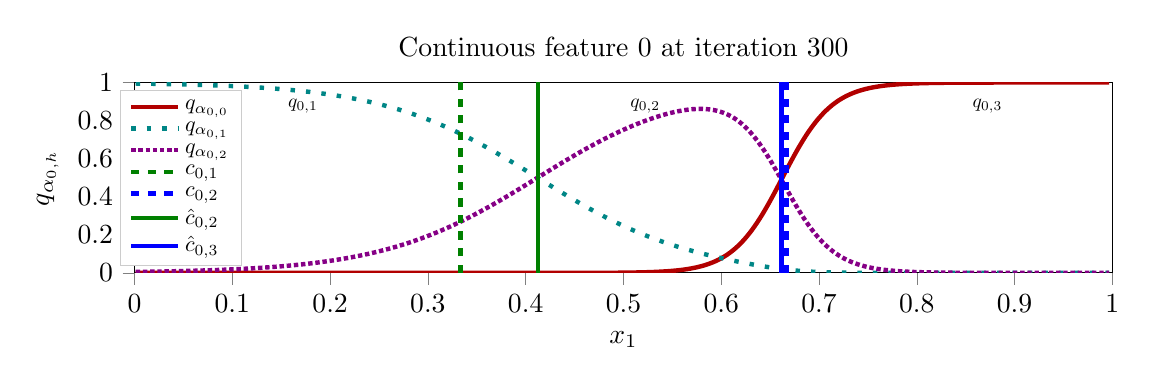
\begin{tikzpicture}

\definecolor{color0}{rgb}{0,0.75,0.75}
\definecolor{color1}{rgb}{0.75,0,0.75}

\begin{axis}[
height=\figureheight,
legend cell align={left},
legend entries={{${q}_{\bm{\alpha}_{0,0}}$},{${q}_{\bm{\alpha}_{0,1}}$},{${q}_{\bm{\alpha}_{0,2}}$},{$c_{0,1}$},{$c_{0,2}$},{$\hat{c}_{0,2}$},{$\hat{c}_{0,3}$}},
legend style={at={(0.11,0.5)}, anchor=east, draw=white!80.0!black, nodes={scale=0.8, transform shape}},
tick align=outside,
tick pos=left,
title={Continuous feature 0 at iteration 300},
width=\figurewidth,
x grid style={white!69.01960784313725!black},
xlabel={$x_1$},
xmin=0, xmax=1,
y grid style={white!69.01960784313725!black},
ylabel={${q}_{\bm{\alpha}_{0,h}}$},
ymin=0, ymax=1
]
\addlegendimage{no markers, ultra thick, red!70.0!black}
\addlegendimage{no markers, ultra thick, loosely dotted, color0!70.0!black}
\addlegendimage{no markers, ultra thick, densely dotted, color1!70.0!black}
\addlegendimage{no markers, ultra thick, dashed, green!50.0!black}
\addlegendimage{no markers, ultra thick, dashed, blue}
\addlegendimage{no markers, ultra thick, green!50.0!black}
\addlegendimage{no markers, ultra thick, blue}
\addplot [ultra thick, red!70.0!black]
table [row sep=\\]{%
0.00121733135182733	3.63606409250258e-14 \\
0.00399800202767708	4.19677754191512e-14 \\
0.00428590830880138	4.25955318651521e-14 \\
0.00583511703754613	4.61384572312141e-14 \\
0.00722810751864345	4.95750460810778e-14 \\
0.00883092408680852	5.38469822116555e-14 \\
0.00892196292255498	5.41002755560707e-14 \\
0.0091566517099908	5.47591486044219e-14 \\
0.00923090984674624	5.49691788940231e-14 \\
0.0100966686316811	5.74789239642104e-14 \\
0.0121625222007031	6.39403555601457e-14 \\
0.0145607215360531	7.23571186691044e-14 \\
0.0148124296089015	7.33024413195581e-14 \\
0.0155108668507814	7.59904969895378e-14 \\
0.016388930761377	7.95100069768059e-14 \\
0.0165505671244613	8.0175483494014e-14 \\
0.0171573414191398	8.2723582216053e-14 \\
0.0193168803366051	9.24669073406291e-14 \\
0.0196176080342491	9.39118235759005e-14 \\
0.0199828289521065	9.56969353478436e-14 \\
0.0217553532903839	1.04854459262362e-13 \\
0.0218823859122642	1.05543300336387e-13 \\
0.0228894296421823	1.11167965024389e-13 \\
0.0231678236934525	1.12775003365765e-13 \\
0.0234639524336395	1.14509638750315e-13 \\
0.0240819943997985	1.18217230709455e-13 \\
0.0245627106801373	1.21183472328104e-13 \\
0.0245889454935851	1.21347620537018e-13 \\
0.0254639162068063	1.26946427003206e-13 \\
0.0259388906266036	1.30093188283574e-13 \\
0.0263836623637999	1.33110468719493e-13 \\
0.0270972950820486	1.38098774494881e-13 \\
0.0283300913612849	1.47159641785723e-13 \\
0.0286622934193979	1.49701635094278e-13 \\
0.0298828118815666	1.5942232072224e-13 \\
0.0300746747069074	1.61007085485235e-13 \\
0.0311555148727282	1.70231829934447e-13 \\
0.0317077923073903	1.75147439954171e-13 \\
0.0332701482181197	1.89835723096027e-13 \\
0.0342621296009059	1.9979414715536e-13 \\
0.0343279985540969	2.00473399816423e-13 \\
0.0344243967448893	2.01472234620352e-13 \\
0.0345313526152026	2.02585520516115e-13 \\
0.0348501916637685	2.05942034259277e-13 \\
0.0349907508243421	2.07439439432223e-13 \\
0.0359872504585017	2.183719513809e-13 \\
0.0362310024928287	2.21132140376668e-13 \\
0.0366095524509532	2.25489142332072e-13 \\
0.0379176486074634	2.41214952742888e-13 \\
0.0403385868224699	2.73267357093349e-13 \\
0.0409980934669582	2.82714471408138e-13 \\
0.0411009563963477	2.8421690456866e-13 \\
0.0416433618426197	2.92272662235499e-13 \\
0.0434312735145819	3.20479645425642e-13 \\
0.0441433900213135	3.32457667081773e-13 \\
0.0453507593315232	3.53797205291176e-13 \\
0.0465425722547385	3.76204113434336e-13 \\
0.048055790853058	4.06708846288628e-13 \\
0.0498244429652048	4.45509541801073e-13 \\
0.0499138395223641	4.47566381742495e-13 \\
0.0500224768452724	4.50077881864949e-13 \\
0.0501451025944044	4.52930770146465e-13 \\
0.0508313343201909	4.69229472985222e-13 \\
0.0528287617134601	5.20084409566524e-13 \\
0.0554318613335167	5.9471362296587e-13 \\
0.0568944168268039	6.41246604426993e-13 \\
0.0580421671310021	6.80297506695793e-13 \\
0.0581829367774224	6.85248353286122e-13 \\
0.0582464981538736	6.87493952825774e-13 \\
0.061138324915142	7.97906012095506e-13 \\
0.0661100314140015	1.03071294988571e-12 \\
0.0666057899124018	1.05736263928541e-12 \\
0.0669707761967708	1.07742157209878e-12 \\
0.0671266686577333	1.08610407993648e-12 \\
0.0686662733539142	1.17570005380568e-12 \\
0.0692515177638677	1.21166694299485e-12 \\
0.0700522852791065	1.26266401848096e-12 \\
0.0708166409087652	1.31333919434207e-12 \\
0.0739831283273903	1.5458527470244e-12 \\
0.0744557758040519	1.58392288000797e-12 \\
0.0760071681977798	1.71558806657396e-12 \\
0.076598016264572	1.76856272682269e-12 \\
0.0770973657055851	1.81460120367294e-12 \\
0.0783565293465318	1.93608930970646e-12 \\
0.078406381150142	1.94106384611425e-12 \\
0.0784226663514104	1.94268733044733e-12 \\
0.0801910475982274	2.12778015692972e-12 \\
0.0811497869224936	2.23538418678282e-12 \\
0.0820428097289791	2.34050365893745e-12 \\
0.0824186797205529	2.38620820151858e-12 \\
0.0842277962246097	2.61899269632382e-12 \\
0.0860509183129933	2.87653950138689e-12 \\
0.0871811255235175	3.04874333244276e-12 \\
0.0878315304280046	3.15248022998704e-12 \\
0.0887988354863684	3.31330514240225e-12 \\
0.0897338519259113	3.47655563191773e-12 \\
0.0899271697891475	3.51129412004547e-12 \\
0.0919787717665748	3.90206617018052e-12 \\
0.0935526652379582	4.2310412985691e-12 \\
0.0939090065052064	4.30929337352781e-12 \\
0.0945988870347061	4.4649167176003e-12 \\
0.096618912882444	4.95363862776377e-12 \\
0.0970084891114591	5.05386878180136e-12 \\
0.0984122603995672	5.43211352635464e-12 \\
0.100207604620953	5.95734832992134e-12 \\
0.100212527088041	5.95886361087761e-12 \\
0.100799383077452	6.14136692889122e-12 \\
0.102777212518229	6.79858773444675e-12 \\
0.10355794511468	7.07695187174284e-12 \\
0.103777986851009	7.15744130630469e-12 \\
0.104283245534613	7.34574207017502e-12 \\
0.104926828677962	7.59276842787759e-12 \\
0.105048147684541	7.6402573503942e-12 \\
0.105888629613813	7.97749886982668e-12 \\
0.106594265398706	8.27207746745273e-12 \\
0.107659824617846	8.73763734976496e-12 \\
0.108236845622617	9.00059714259438e-12 \\
0.108525705010578	9.13519086764847e-12 \\
0.110299453724928	1.00068165559408e-11 \\
0.1109411277088	1.03421802372106e-11 \\
0.114327603236688	1.23072151428372e-11 \\
0.114459519996847	1.23908877949774e-11 \\
0.117867979538534	1.47612356365956e-11 \\
0.118112325438648	1.49476021837902e-11 \\
0.118633260119092	1.53528110363732e-11 \\
0.11982692170167	1.63231754501947e-11 \\
0.120297266407184	1.67221583802224e-11 \\
0.12058353024893	1.69697589313955e-11 \\
0.120831487175604	1.71871267218293e-11 \\
0.12100766940383	1.73432709166255e-11 \\
0.121149329304323	1.74698987914779e-11 \\
0.12132073351728	1.76242943850102e-11 \\
0.124248653311104	2.04824820299043e-11 \\
0.126006965902748	2.24167490125993e-11 \\
0.126901124475677	2.34692786038604e-11 \\
0.126954279439678	2.35333679626804e-11 \\
0.128893135931382	2.59949943515192e-11 \\
0.129130414500304	2.63133386607661e-11 \\
0.129265754179532	2.64966572988135e-11 \\
0.129318382573767	2.65682927047539e-11 \\
0.12957327546953	2.69180632644916e-11 \\
0.129620549409663	2.69833738686387e-11 \\
0.130028516874333	2.75540926880646e-11 \\
0.131097613537266	2.91074490899046e-11 \\
0.133250294991105	3.25055156402687e-11 \\
0.13328775473883	3.25680073187673e-11 \\
0.13407228993995	3.39051599296258e-11 \\
0.134949207751391	3.54645653122265e-11 \\
0.138173080751483	4.18390322387552e-11 \\
0.138829427196237	4.32707099318197e-11 \\
0.13934817040543	4.4436739010667e-11 \\
0.140500928037371	4.71415025071753e-11 \\
0.141075328307274	4.85499383751087e-11 \\
0.142185810887561	5.13929732104401e-11 \\
0.143422034202274	5.47539479034409e-11 \\
0.143493165626466	5.49538678451533e-11 \\
0.144195876538432	5.69684785456381e-11 \\
0.148766937684016	7.1998497441772e-11 \\
0.150763038004328	7.97468271973578e-11 \\
0.151522077107299	8.29071533647863e-11 \\
0.152255804124635	8.60805871027992e-11 \\
0.15226616541564	8.61261756357479e-11 \\
0.153023332064105	8.9529945956901e-11 \\
0.153075622362746	8.97699345414615e-11 \\
0.153205273538633	9.03675814734051e-11 \\
0.155085023545417	9.94939131082617e-11 \\
0.15772483711392	1.13883083519006e-10 \\
0.158186389101905	1.16604295663514e-10 \\
0.15894693490281	1.21230317451371e-10 \\
0.159639800043974	1.25603999423518e-10 \\
0.160146141938642	1.28899627083179e-10 \\
0.160729957792949	1.32806515784623e-10 \\
0.160844366590924	1.33585892347909e-10 \\
0.16282671011704	1.47837880826174e-10 \\
0.163830519374535	1.55622917330511e-10 \\
0.163992249762284	1.56915216931175e-10 \\
0.164417055397194	1.60360308365526e-10 \\
0.165260696441198	1.67426683628236e-10 \\
0.167361304418963	1.86402143720343e-10 \\
0.169491743858274	2.07837594357052e-10 \\
0.170198366879178	2.1547734430083e-10 \\
0.17056212452737	2.19518347943648e-10 \\
0.170912119394526	2.23478083261064e-10 \\
0.172648789750251	2.44205211608062e-10 \\
0.172856178369217	2.46805353931734e-10 \\
0.173162955842619	2.50701182036295e-10 \\
0.173717258172562	2.57898036259974e-10 \\
0.174916773476619	2.74185424364859e-10 \\
0.175269110850529	2.79161915806014e-10 \\
0.175796530948979	2.86779017200089e-10 \\
0.176965388380551	3.044076934966e-10 \\
0.177321345888588	3.09988923419269e-10 \\
0.177435150590059	3.11793590945797e-10 \\
0.178853029237583	3.35187100297674e-10 \\
0.179003818378901	3.37776362435704e-10 \\
0.180108329801849	3.57354562607881e-10 \\
0.18098127250095	3.73626574123875e-10 \\
0.181164449059833	3.77132991502549e-10 \\
0.181504936132438	3.8373887401022e-10 \\
0.181698184610282	3.8754044417999e-10 \\
0.181706779152786	3.87709836457972e-10 \\
0.183508352968371	4.2501413499707e-10 \\
0.18371338802759	4.29480395691684e-10 \\
0.184634680521775	4.5013270888461e-10 \\
0.18715264530893	5.11766851118978e-10 \\
0.187902267731003	5.31691857208472e-10 \\
0.188039517539109	5.35422373104666e-10 \\
0.18935042046278	5.72399017073622e-10 \\
0.190047732419662	5.93093463230332e-10 \\
0.190622119303773	6.10698103198359e-10 \\
0.191971593527005	6.54137133349053e-10 \\
0.193283500603906	6.993166046243e-10 \\
0.197644387198593	8.73052574679178e-10 \\
0.19852231723701	9.12917685891301e-10 \\
0.200336272290021	1.00112085288373e-09 \\
0.200653415987652	1.01739294766645e-09 \\
0.20282835566531	1.13630527209807e-09 \\
0.205443999059423	1.29777921742402e-09 \\
0.207292923022167	1.42551870307983e-09 \\
0.208117425413999	1.48644829778277e-09 \\
0.210007644411429	1.63610158754324e-09 \\
0.213557102615423	1.95882354780963e-09 \\
0.215277579547195	2.13732787024412e-09 \\
0.215497345364033	2.16126339047662e-09 \\
0.216310718872085	2.25220508909274e-09 \\
0.216355091614949	2.25727259106634e-09 \\
0.217392921106891	2.37913155842762e-09 \\
0.217574656587144	2.40113906535555e-09 \\
0.22044293838767	2.77648259938701e-09 \\
0.220716468008851	2.81519541012187e-09 \\
0.222115983638242	3.02182279199315e-09 \\
0.222246464423612	3.04183900290411e-09 \\
0.22273747409856	3.11835357535983e-09 \\
0.224665735391259	3.43782424749861e-09 \\
0.226091799609793	3.69485531059865e-09 \\
0.226553200069555	3.78204756401601e-09 \\
0.227270480715813	3.92166965568208e-09 \\
0.227447153120765	3.95684152110221e-09 \\
0.227729308234277	4.01365429780753e-09 \\
0.228445973454936	4.16165013561454e-09 \\
0.230001408006134	4.50179671318551e-09 \\
0.230452444453415	4.60551774494888e-09 \\
0.23101774976842	4.73886707652582e-09 \\
0.232175303582309	5.02401764634897e-09 \\
0.238608988543593	6.94944946033615e-09 \\
0.238816890215772	7.02263003304893e-09 \\
0.241051513831921	7.85916309808954e-09 \\
0.24158011969787	8.07109401534944e-09 \\
0.241902400534758	8.2030870984795e-09 \\
0.245972048559771	1.00666230906654e-08 \\
0.246055548554611	1.0108967885003e-08 \\
0.246667080102265	1.04245225784894e-08 \\
0.249063142333596	1.17581402392375e-08 \\
0.2492389743227	1.18624088329966e-08 \\
0.250289311607262	1.25048300603225e-08 \\
0.250515586119678	1.2647663361065e-08 \\
0.250940657287891	1.2920406078365e-08 \\
0.25167183440657	1.3403346876828e-08 \\
0.257990385058828	1.83979214085639e-08 \\
0.258124141751891	1.85215665027272e-08 \\
0.258177043220415	1.85706738875524e-08 \\
0.259695612003727	2.00374081771315e-08 \\
0.259776131366315	2.0118301691241e-08 \\
0.260071715391803	2.04180157226119e-08 \\
0.261863459876915	2.23324931880597e-08 \\
0.262327493161023	2.28567191840057e-08 \\
0.26759593699964	2.97369435742212e-08 \\
0.268489073403659	3.10918295554075e-08 \\
0.268717231393198	3.14476835683308e-08 \\
0.268959947078319	3.18306767610466e-08 \\
0.270587931966637	3.45219817177167e-08 \\
0.270690946459964	3.46997168776397e-08 \\
0.271962599626952	3.69693964330509e-08 \\
0.272078011383322	3.71826054390567e-08 \\
0.273472308124372	3.98559834025036e-08 \\
0.2748160216297	4.26124984187481e-08 \\
0.27486022346705	4.27062438745907e-08 \\
0.276792319224663	4.70135326224863e-08 \\
0.277649825865711	4.90607163783352e-08 \\
0.278253018986364	5.05535737715945e-08 \\
0.278408961673642	5.09467099618632e-08 \\
0.280420535697693	5.62988660135488e-08 \\
0.280986539769637	5.79027350511296e-08 \\
0.282010151037797	6.09194046319317e-08 \\
0.282040248224806	6.10104251563826e-08 \\
0.282123909223068	6.12642025998866e-08 \\
0.285513331048722	7.24710531585515e-08 \\
0.287573265929611	8.02510840003379e-08 \\
0.288706085955357	8.48765822070163e-08 \\
0.290405917039397	9.23170304645282e-08 \\
0.290997388676799	9.50545810951553e-08 \\
0.291345467206721	9.67030828746829e-08 \\
0.291398859476294	9.69584803556245e-08 \\
0.291913353201399	9.94536222265197e-08 \\
0.292457883757979	1.02163632220709e-07 \\
0.293034823854815	1.05114814630269e-07 \\
0.293967194785546	1.10063453462317e-07 \\
0.294530422037374	1.13164098536345e-07 \\
0.294989677655505	1.15756030538705e-07 \\
0.297159059538413	1.28816651567831e-07 \\
0.297297208003757	1.29696189787865e-07 \\
0.297401117461309	1.30361698325032e-07 \\
0.297596325223743	1.31620765841944e-07 \\
0.297864053288129	1.3336739357328e-07 \\
0.30177729109265	1.61674648779808e-07 \\
0.303412381953207	1.7519418804568e-07 \\
0.303804315308251	1.78597545641423e-07 \\
0.304062576428461	1.80875730393382e-07 \\
0.305272733951204	1.91940202398655e-07 \\
0.308571936874729	2.25620581773001e-07 \\
0.308642296164111	2.26399436087377e-07 \\
0.308753468839242	2.27634913585462e-07 \\
0.313549155412623	2.87780665075843e-07 \\
0.313653278508487	2.89247651608093e-07 \\
0.314321905263844	2.98843332302567e-07 \\
0.315143369330536	3.11063928393196e-07 \\
0.315610968893992	3.18239386842833e-07 \\
0.315614001089602	3.18286708989035e-07 \\
0.316213538079681	3.27727804005917e-07 \\
0.31656704193251	3.3342354299748e-07 \\
0.317033096183104	3.41082539989657e-07 \\
0.318077975465148	3.58892691565416e-07 \\
0.318499630211901	3.66336053048144e-07 \\
0.320459324952121	4.0298536418959e-07 \\
0.321158026386313	4.16909159639545e-07 \\
0.324068371830885	4.80199730645836e-07 \\
0.325719114944994	5.2022176078026e-07 \\
0.32726449148383	5.60664943805023e-07 \\
0.327515376124492	5.67516963201342e-07 \\
0.328913020135104	6.07231470439729e-07 \\
0.329471410393436	6.23853395609331e-07 \\
0.329483556970732	6.24220604095171e-07 \\
0.329807282212852	6.34067248483916e-07 \\
0.330833599133424	6.66311564145872e-07 \\
0.33305761718435	7.41836004181096e-07 \\
0.334466305551428	7.93978358615277e-07 \\
0.336209591213773	8.63532704897807e-07 \\
0.339174876956243	9.95900450107001e-07 \\
0.339882470276715	1.0303332373951e-06 \\
0.34038186985453	1.05533854366513e-06 \\
0.341801626815983	1.12973873456212e-06 \\
0.343524436417214	1.22699077564903e-06 \\
0.343689611464564	1.23673839880212e-06 \\
0.344781691139359	1.30312309920555e-06 \\
0.345591136214371	1.35458355998708e-06 \\
0.346919336340971	1.44339276175742e-06 \\
0.347671848387079	1.49622940170957e-06 \\
0.348163376208385	1.53176574713143e-06 \\
0.349472519093074	1.63051925028412e-06 \\
0.349745522231846	1.65188896517066e-06 \\
0.351374549797252	1.78526022409642e-06 \\
0.35188450877064	1.8291522110303e-06 \\
0.356410987959693	2.26830252358923e-06 \\
0.357063359912744	2.33961077356071e-06 \\
0.35766224198294	2.40701274378807e-06 \\
0.359634636963466	2.64278787653893e-06 \\
0.359702418340943	2.65128392129554e-06 \\
0.360059525411196	2.69648103312647e-06 \\
0.360289892612103	2.72603870143939e-06 \\
0.360991066472348	2.81797588286281e-06 \\
0.361517661936521	2.88902447209693e-06 \\
0.362811795477131	3.07119921671983e-06 \\
0.363672312199373	3.19854143526754e-06 \\
0.364539422226955	3.33210709868581e-06 \\
0.364777329717716	3.36969901582052e-06 \\
0.366260111813999	3.61360298484215e-06 \\
0.366299975782456	3.62039145329618e-06 \\
0.366824068875263	3.71085207007127e-06 \\
0.366852341843951	3.71579085367557e-06 \\
0.367255430778636	3.7869699553994e-06 \\
0.367718612255156	3.87041654903442e-06 \\
0.371844893263566	4.69815950054908e-06 \\
0.373914699139864	5.17659100296441e-06 \\
0.375334232083758	5.53207792108878e-06 \\
0.375994866909118	5.70559222978773e-06 \\
0.376668338720068	5.88797047385015e-06 \\
0.377076405033397	6.00126213612384e-06 \\
0.377984484345733	6.26109385848395e-06 \\
0.378411364752534	6.38701840216527e-06 \\
0.378781645976558	6.4982755247911e-06 \\
0.378969500633152	6.55544681649189e-06 \\
0.380503918700316	7.04125841366476e-06 \\
0.382290922993942	7.65172171668382e-06 \\
0.382702553179553	7.79954825702589e-06 \\
0.384322573332172	8.4090379459667e-06 \\
0.385259749331941	8.78272476256825e-06 \\
0.387372760421529	9.68613312579691e-06 \\
0.387555538130506	9.76842511590803e-06 \\
0.38907064039843	1.04775981526473e-05 \\
0.389579566720786	1.07269725049264e-05 \\
0.389767492364477	1.08205103970249e-05 \\
0.392492189498792	1.22702440421563e-05 \\
0.393836249332015	1.30539619931369e-05 \\
0.395499606909982	1.40921456477372e-05 \\
0.395882251973212	1.4342167560244e-05 \\
0.396415701753994	1.46980837598676e-05 \\
0.396441121576172	1.47152604768053e-05 \\
0.396574304024945	1.48055432873662e-05 \\
0.397759074483525	1.56330934260041e-05 \\
0.39792914466779	1.57555296027567e-05 \\
0.39903214396726	1.65729015861871e-05 \\
0.399785344239434	1.71548053913284e-05 \\
0.400492759495042	1.77195652213413e-05 \\
0.401432469526815	1.84980708581861e-05 \\
0.401683506422962	1.87116238521412e-05 \\
0.403117526972048	1.99789137695916e-05 \\
0.403655328822729	2.04755215236219e-05 \\
0.404677310156115	2.14528772630729e-05 \\
0.404776114127771	2.15498257603031e-05 \\
0.409382548454498	2.6575840820442e-05 \\
0.409383683968994	2.65772378043039e-05 \\
0.411266446539173	2.89477447950048e-05 \\
0.413513881114749	3.20497674692888e-05 \\
0.415418916892999	3.4932658309117e-05 \\
0.415684791078115	3.53547075064853e-05 \\
0.415897400040632	3.56957098119892e-05 \\
0.416751124277095	3.70981033483986e-05 \\
0.420526451622837	4.39750474470202e-05 \\
0.421389674091991	4.57150053989608e-05 \\
0.422435717298333	4.79139307572041e-05 \\
0.425131879618846	5.40709406777751e-05 \\
0.426344701070752	5.7087167078862e-05 \\
0.42646767360874	5.74021723878104e-05 \\
0.426723043204646	5.80615196668077e-05 \\
0.427177869701464	5.92544201936107e-05 \\
0.427843332102008	6.10429851803929e-05 \\
0.430519905858631	6.87867868691683e-05 \\
0.431329847429739	7.13142362656072e-05 \\
0.43280912191732	7.61674527893774e-05 \\
0.435328420042426	8.51881268317811e-05 \\
0.437335390870841	9.31160611798987e-05 \\
0.438093952949238	9.62971898843534e-05 \\
0.438539868644415	9.82166311587207e-05 \\
0.438622154375097	9.85747101367451e-05 \\
0.440101706010519	0.000105239727417938 \\
0.441692841095718	0.000112900037493091 \\
0.442760304995134	0.000118342977657449 \\
0.443866566189192	0.000124254715046845 \\
0.445656815071723	0.000134440211695619 \\
0.446306999832311	0.000138338349643163 \\
0.446539778293263	0.000139760915772058 \\
0.447015636734589	0.000142713150125928 \\
0.447764619143311	0.000147484301123768 \\
0.450701475867445	0.000167747974046506 \\
0.451256246885538	0.00017187102639582 \\
0.452657062023863	0.000182729156222194 \\
0.453713810202396	0.000191362225450575 \\
0.455679938271804	0.000208502198802307 \\
0.458387666537298	0.000234590828767978 \\
0.458683449593184	0.000237627711612731 \\
0.458715521584147	0.000237958869547583 \\
0.461316576778666	0.000266415911028162 \\
0.461325542738979	0.000266520015429705 \\
0.463543573073144	0.000293411314487457 \\
0.465979585607885	0.00032601464772597 \\
0.467407797462426	0.000346754124620929 \\
0.468691827800416	0.000366501073585823 \\
0.468898574730863	0.000369781657354906 \\
0.472124347134469	0.000424863072112203 \\
0.473167350177021	0.000444338220404461 \\
0.475892207786094	0.000499439600389451 \\
0.476447833983088	0.000511470716446638 \\
0.476852808050028	0.000520419562235475 \\
0.480153820674186	0.000599319464527071 \\
0.481331481462533	0.000630215334240347 \\
0.481907398972557	0.000645890191663057 \\
0.482340193954975	0.000657919852528721 \\
0.483064633983067	0.000678548123687506 \\
0.484404961256947	0.000718400930054486 \\
0.484965300777859	0.000735735869966447 \\
0.486726527314222	0.000792935432400554 \\
0.487116327031527	0.000806172494776547 \\
0.488921795423616	0.000870367279276252 \\
0.489759269088015	0.000901822815649211 \\
0.490909081458542	0.000946833228226751 \\
0.49091604463621	0.000947113614529371 \\
0.492300495791636	0.00100425770506263 \\
0.4923307300145	0.00100554141681641 \\
0.492381040900871	0.00100768380798399 \\
0.49359088600479	0.00106055825017393 \\
0.493621516312431	0.00106193183455616 \\
0.494440937544777	0.00109932816121727 \\
0.494453842969403	0.00109992758370936 \\
0.495146776944368	0.00113257567863911 \\
0.495982811187486	0.00117323372978717 \\
0.497062669506957	0.00122787558939308 \\
0.497330994039467	0.0012418320402503 \\
0.498153946067205	0.00128562864847481 \\
0.498455749672111	0.00130206730682403 \\
0.498730582702143	0.00131721410434693 \\
0.499638616573585	0.0013685057638213 \\
0.500015331367196	0.00139035237953067 \\
0.501350798827707	0.00147060758899897 \\
0.501744525678089	0.00149511964991689 \\
0.5036535166819	0.00161979382392019 \\
0.504487562746051	0.00167741638142616 \\
0.508463499372222	0.00198096386156976 \\
0.509687293635359	0.00208481587469578 \\
0.509914323813028	0.0021046600304544 \\
0.511341386088067	0.00223371223546565 \\
0.512018604529405	0.00229764683172107 \\
0.513861444023579	0.00248084450140595 \\
0.514960109685398	0.00259681837633252 \\
0.515737002786438	0.00268202251754701 \\
0.519058118042992	0.00307824928313494 \\
0.519916366374704	0.00318965269252658 \\
0.521499066868756	0.00340556888841093 \\
0.52201095621904	0.00347843067720532 \\
0.524040740980263	0.00378270051442087 \\
0.524478728901278	0.00385169801302254 \\
0.525423938335719	0.00400484818965197 \\
0.525635126495304	0.00403986964374781 \\
0.52719728420485	0.00430847564712167 \\
0.52996761968302	0.00482852570712566 \\
0.530301937454978	0.00489531690254807 \\
0.531840017863588	0.00521440617740154 \\
0.531981886047464	0.00524484366178513 \\
0.532012239031215	0.00525137828662992 \\
0.533028472048003	0.00547486264258623 \\
0.533892144890962	0.00567209767177701 \\
0.537533560414064	0.00658311415463686 \\
0.537969095533598	0.00670125940814614 \\
0.538335797788309	0.00680231302976608 \\
0.539116247263892	0.00702242087572813 \\
0.542861601060095	0.00817957334220409 \\
0.54363288334093	0.00844009127467871 \\
0.543801322498743	0.00849803537130356 \\
0.547002474800456	0.00967659149318933 \\
0.548908529730498	0.0104527091607451 \\
0.550793838508607	0.0112800793722272 \\
0.553233155778543	0.0124459750950336 \\
0.554063975822177	0.0128692928701639 \\
0.554664151973859	0.0131838144734502 \\
0.555237937942708	0.0134914889931679 \\
0.556147032749051	0.0139933358877897 \\
0.556971759420448	0.0144643215462565 \\
0.557200406957364	0.0145975733175874 \\
0.557472354513669	0.0147576872259378 \\
0.557634255107793	0.0148537587374449 \\
0.557665270553959	0.0148722780868411 \\
0.558053776980733	0.0151056637987494 \\
0.559718195298125	0.0161465797573328 \\
0.560469384381131	0.0166389364749193 \\
0.561223854392744	0.0171480868011713 \\
0.561301666038306	0.0172014310956001 \\
0.561798210581049	0.0175458155572414 \\
0.562009451463098	0.0176943484693766 \\
0.562833608522221	0.018285546451807 \\
0.564513388059411	0.0195503924041986 \\
0.566269134382303	0.0209629982709885 \\
0.567354059069172	0.0218847263604403 \\
0.567568119614931	0.0220711547881365 \\
0.568027250200944	0.0224762372672558 \\
0.568168895571326	0.0226026196032763 \\
0.568859714229155	0.0232290457934141 \\
0.569040001476579	0.0233952645212412 \\
0.569210703701173	0.0235537309199572 \\
0.56954243172626	0.0238645616918802 \\
0.570337723054723	0.0246260408312082 \\
0.570715244097907	0.0249957405030727 \\
0.57424855250552	0.0287241283804178 \\
0.575002703666514	0.0295865219086409 \\
0.575003549718568	0.0295874886214733 \\
0.575679471524471	0.0303814690560102 \\
0.575807053629817	0.0305335186421871 \\
0.576466959777726	0.0313321948051453 \\
0.576872834170159	0.0318332947790623 \\
0.579766556433004	0.035634521394968 \\
0.580763685611283	0.0370418652892113 \\
0.581439442781873	0.0380255356431007 \\
0.582738039976926	0.0399859845638275 \\
0.583406899826349	0.041032936424017 \\
0.583621843838165	0.0413748137652874 \\
0.584022416391563	0.0420190691947937 \\
0.584157343282694	0.0422382913529873 \\
0.584398535047123	0.0426327474415302 \\
0.588037407975546	0.0490231290459633 \\
0.591515761019391	0.055963609367609 \\
0.59169858018679	0.0563525557518005 \\
0.591779783399284	0.0565261766314507 \\
0.593283454206354	0.0598321780562401 \\
0.593390679676707	0.0600747019052505 \\
0.593962031860602	0.0613820143043995 \\
0.594200655435401	0.0619359575212002 \\
0.596969362786692	0.0687080398201942 \\
0.598437319346411	0.0725683569908142 \\
0.599474715240117	0.0754149407148361 \\
0.602362270570747	0.083879828453064 \\
0.603334150143409	0.0869161635637283 \\
0.603632921169445	0.0878691002726555 \\
0.60379362440282	0.088385708630085 \\
0.604659766964252	0.091216467320919 \\
0.605395322349658	0.0936833992600441 \\
0.606463918589886	0.097372978925705 \\
0.606775419688025	0.0984725132584572 \\
0.607357857377935	0.100557811558247 \\
0.607580561722253	0.101365394890308 \\
0.608621286245357	0.10521524399519 \\
0.609575970841381	0.108858428895473 \\
0.610347066222159	0.111880771815777 \\
0.612177604245754	0.119347505271435 \\
0.613326929015952	0.124250866472721 \\
0.614270777301711	0.128404945135117 \\
0.614798584840558	0.130778461694717 \\
0.616647348049137	0.139385282993317 \\
0.616860752444383	0.14040832221508 \\
0.617045516373702	0.141299307346344 \\
0.618083376848042	0.146390736103058 \\
0.621554333086694	0.164517179131508 \\
0.623029526806788	0.172745227813721 \\
0.624069668412363	0.178738489747047 \\
0.624143156449471	0.179167881608009 \\
0.625318868337709	0.186147511005402 \\
0.627896177690147	0.202169418334961 \\
0.62805232111942	0.203171774744987 \\
0.629405663035747	0.212016001343727 \\
0.629846029847146	0.214952990412712 \\
0.630467114324592	0.219144865870476 \\
0.630546820907001	0.219686910510063 \\
0.631083637650338	0.223363250494003 \\
0.631324147788059	0.225024193525314 \\
0.632680726177628	0.23455522954464 \\
0.632823775680698	0.23557610809803 \\
0.633074796432523	0.237375393509865 \\
0.636612707474017	0.26371431350708 \\
0.639030758002587	0.282747894525528 \\
0.640237995740933	0.292552292346954 \\
0.640853111920735	0.297623068094254 \\
0.640965174455041	0.298552066087723 \\
0.641077861086201	0.299487978219986 \\
0.641318662912942	0.30149382352829 \\
0.642222835181407	0.30909064412117 \\
0.64234387506577	0.310116112232208 \\
0.643801671660635	0.322603464126587 \\
0.644160446263096	0.32571604847908 \\
0.645423350530499	0.336792945861816 \\
0.646045259468861	0.342314273118973 \\
0.646175373815422	0.343474745750427 \\
0.646229368496451	0.343956828117371 \\
0.64633540284767	0.344904959201813 \\
0.647248616680538	0.353116720914841 \\
0.647279370177658	0.353395074605942 \\
0.648437609650589	0.36393791437149 \\
0.648804842952185	0.367308050394058 \\
0.650925300722929	0.387009590864182 \\
0.651147043039429	0.389092594385147 \\
0.651662018637987	0.393944203853607 \\
0.651706157147625	0.39436075091362 \\
0.654010541995451	0.416317909955978 \\
0.654559822635481	0.421603560447693 \\
0.655118993248004	0.427001923322678 \\
0.655470347269005	0.43040332198143 \\
0.656959015265393	0.444879144430161 \\
0.657756536283002	0.452673405408859 \\
0.65779828590582	0.453082591295242 \\
0.657827620225886	0.453369587659836 \\
0.657888612459039	0.453966408967972 \\
0.659397129207233	0.468772709369659 \\
0.660938309454123	0.48395299911499 \\
0.661236182036626	0.486890196800232 \\
0.661269452289108	0.487218081951141 \\
0.662216186165834	0.496559917926788 \\
0.662950819650895	0.503809571266174 \\
0.66338057911196	0.508049368858337 \\
0.663432705107081	0.508564114570618 \\
0.663724169525683	0.511439144611359 \\
0.663888183512934	0.513056099414825 \\
0.664768718946012	0.521732270717621 \\
0.665166852000189	0.525651693344116 \\
0.667536155027696	0.54888516664505 \\
0.667706149437679	0.550544559955597 \\
0.668306929681857	0.556401431560516 \\
0.669748926816749	0.57038801908493 \\
0.670170670738544	0.574458718299866 \\
0.67145696403461	0.586806535720825 \\
0.672338548572371	0.595206379890442 \\
0.673491333278333	0.606104254722595 \\
0.67403307442415	0.611189424991608 \\
0.674416791668541	0.61477667093277 \\
0.674787425171747	0.618229687213898 \\
0.676446369741635	0.633533179759979 \\
0.677562284895504	0.643677651882172 \\
0.678599282385815	0.652989506721497 \\
0.678826329178824	0.655012726783752 \\
0.67896152739786	0.656214475631714 \\
0.67899511965357	0.656513154506683 \\
0.680140229601849	0.666609048843384 \\
0.682444051919919	0.686453104019165 \\
0.683867370343219	0.698383927345276 \\
0.684052257749766	0.699914038181305 \\
0.684255695186768	0.701593339443207 \\
0.685029448440209	0.707928597927094 \\
0.685031601583854	0.707946538925171 \\
0.686087221986552	0.716460287570953 \\
0.686595026192521	0.720501184463501 \\
0.688706229954925	0.736916780471802 \\
0.68873272487683	0.737118721008301 \\
0.689123647830945	0.740087330341339 \\
0.689304555740157	0.741453468799591 \\
0.690587617264716	0.751009225845337 \\
0.692311859501987	0.763470709323883 \\
0.695700743349649	0.78667938709259 \\
0.695837298048015	0.787578880786896 \\
0.696457522478708	0.791628122329712 \\
0.697811144019126	0.800267100334167 \\
0.699552387539892	0.810978889465332 \\
0.699842672845189	0.812720954418182 \\
0.700339206753902	0.815671563148499 \\
0.703914523708911	0.83585798740387 \\
0.704439323787712	0.838666200637817 \\
0.70518880951018	0.842608571052551 \\
0.7071797083437	0.852700293064117 \\
0.708834257241349	0.860672652721405 \\
0.711812884354997	0.874110162258148 \\
0.713800787712356	0.882446050643921 \\
0.714381295666559	0.88478821516037 \\
0.714553460198799	0.885475218296051 \\
0.71617759911668	0.891779541969299 \\
0.716279214056233	0.892163634300232 \\
0.71706526463665	0.895094573497772 \\
0.7170774036456	0.895139157772064 \\
0.718797169833086	0.901304125785828 \\
0.719928747300243	0.905182123184204 \\
0.720015265610924	0.905472993850708 \\
0.720180585299769	0.906026422977448 \\
0.720486724533789	0.907043516635895 \\
0.720811625371112	0.908112287521362 \\
0.721884477676013	0.911562860012054 \\
0.722674846752593	0.914029598236084 \\
0.723407083196464	0.916258931159973 \\
0.72376333377458	0.917324542999268 \\
0.723777685375425	0.917366981506348 \\
0.724101671418291	0.918324828147888 \\
0.725216929943891	0.921544551849365 \\
0.726260808708396	0.924452304840088 \\
0.727196308633524	0.926974058151245 \\
0.728279458765382	0.929796040058136 \\
0.728773876001269	0.931050419807434 \\
0.73010645683466	0.934328436851501 \\
0.730325657495659	0.934853315353394 \\
0.731103800769119	0.936685919761658 \\
0.732842907312836	0.94060891866684 \\
0.733030886031315	0.941019058227539 \\
0.733363211301201	0.941737532615662 \\
0.733408558006162	0.941834926605225 \\
0.733541706051593	0.942119956016541 \\
0.736646424210889	0.948406159877777 \\
0.737257987460932	0.949565947055817 \\
0.737740868508229	0.950464010238647 \\
0.739663624018122	0.953891515731812 \\
0.740427472376599	0.955189645290375 \\
0.74048368334169	0.955283582210541 \\
0.741199257625272	0.956465423107147 \\
0.742026689151921	0.957794785499573 \\
0.742109660962147	0.957925915718079 \\
0.743260964407579	0.959705710411072 \\
0.745904906945693	0.963523387908936 \\
0.74602435830571	0.963687419891357 \\
0.746454517124051	0.964272201061249 \\
0.746519724823025	0.964359998703003 \\
0.746876733445386	0.964837193489075 \\
0.74711794423622	0.965156197547913 \\
0.747724262896222	0.965945541858673 \\
0.748345753702398	0.966736793518066 \\
0.751166500773878	0.970109641551971 \\
0.751791977276396	0.970811367034912 \\
0.75209959948437	0.971150398254395 \\
0.754656199772114	0.973825037479401 \\
0.755352629585724	0.974510848522186 \\
0.755545959822728	0.974698126316071 \\
0.755898419561934	0.975035965442657 \\
0.75953948606339	0.978278398513794 \\
0.759789627332931	0.978485405445099 \\
0.761184688869922	0.979604601860046 \\
0.762076488879603	0.980289995670319 \\
0.764704611561162	0.982181072235107 \\
0.766584586955775	0.983423113822937 \\
0.766717023391223	0.983507394790649 \\
0.76740816183118	0.983940005302429 \\
0.767805205005891	0.984183669090271 \\
0.768945200187728	0.984862625598907 \\
0.769095248498746	0.984949946403503 \\
0.771115505162259	0.986077070236206 \\
0.77123453886572	0.986140847206116 \\
0.772690297390309	0.986897587776184 \\
0.772800656010738	0.986953258514404 \\
0.773541775943403	0.987321138381958 \\
0.774318112411085	0.987695574760437 \\
0.774382414958023	0.987726032733917 \\
0.775966989001763	0.988454699516296 \\
0.776941567881457	0.988881528377533 \\
0.777151204151402	0.988971173763275 \\
0.77925160646798	0.989831626415253 \\
0.781696335832752	0.990749657154083 \\
0.782369539728008	0.990987718105316 \\
0.783725295642214	0.991448819637299 \\
0.783923601908101	0.991514325141907 \\
0.784737906340657	0.991777896881104 \\
0.785900126610763	0.992140114307404 \\
0.790961807063793	0.993541240692139 \\
0.793304211192844	0.994102776050568 \\
0.793342107282624	0.994111478328705 \\
0.796510242295205	0.994793355464935 \\
0.798772767293139	0.995231688022614 \\
0.800222874557644	0.995493054389954 \\
0.800675457983639	0.995571613311768 \\
0.801306704659443	0.995679080486298 \\
0.801480486720766	0.995708107948303 \\
0.801719692000218	0.995747864246368 \\
0.80195867569636	0.99578732252121 \\
0.802469344823613	0.995870053768158 \\
0.803160899528724	0.9959796667099 \\
0.803630989013321	0.996052503585815 \\
0.803732818796934	0.996068120002747 \\
0.804155707385168	0.996132254600525 \\
0.804850691603272	0.996235430240631 \\
0.805686471533716	0.996356010437012 \\
0.806516792766975	0.996471762657166 \\
0.807556103824507	0.996611654758453 \\
0.809371349985681	0.996842741966248 \\
0.810657337863434	0.996996998786926 \\
0.81238276958492	0.997191965579987 \\
0.815136873135806	0.99747759103775 \\
0.816535913131519	0.997611403465271 \\
0.816918806227773	0.997646629810333 \\
0.817084298588666	0.997661828994751 \\
0.817334232802015	0.997684359550476 \\
0.817404874574028	0.997690796852112 \\
0.818917146623526	0.997822880744934 \\
0.819939989256465	0.997907996177673 \\
0.820379410487342	0.997943460941315 \\
0.820978701871047	0.997990965843201 \\
0.821259126029298	0.998012661933899 \\
0.82294611725228	0.998139142990112 \\
0.82486764275723	0.998273372650146 \\
0.825081200240856	0.998287737369537 \\
0.826218307949063	0.998361885547638 \\
0.827593135154276	0.998447358608246 \\
0.828249382527173	0.998486518859863 \\
0.830013952508867	0.998587131500244 \\
0.83098818774312	0.998639762401581 \\
0.831688198955698	0.998676359653473 \\
0.832565489851338	0.998720824718475 \\
0.833166954421711	0.998750567436218 \\
0.834321464969713	0.998805522918701 \\
0.834662447919532	0.998821318149567 \\
0.834802486072627	0.998827755451202 \\
0.836038817557475	0.998882830142975 \\
0.841215178556551	0.999086976051331 \\
0.842621481063247	0.999135673046112 \\
0.843756311857548	0.999173104763031 \\
0.844078008814596	0.999183356761932 \\
0.845960625476654	0.999241232872009 \\
0.846191469096939	0.999247968196869 \\
0.847407394156738	0.999282896518707 \\
0.848536745674345	0.999313712120056 \\
0.848886286362396	0.999323010444641 \\
0.849381960450326	0.999335944652557 \\
0.849923846134606	0.999349892139435 \\
0.85007572166574	0.9993537068367 \\
0.851439281652725	0.99938702583313 \\
0.854113156525351	0.999447762966156 \\
0.855218609206591	0.999471127986908 \\
0.856710132316332	0.99950098991394 \\
0.856932509485749	0.999505281448364 \\
0.85749564495731	0.999516129493713 \\
0.859409177005295	0.999550759792328 \\
0.859979894092921	0.999560654163361 \\
0.860467004421787	0.999568998813629 \\
0.861163762259384	0.999580562114716 \\
0.861665377957976	0.999588668346405 \\
0.863178775146987	0.999612271785736 \\
0.864132337960544	0.999626398086548 \\
0.865438728206212	0.999644994735718 \\
0.866581901348173	0.99966037273407 \\
0.86858392562578	0.999686002731323 \\
0.86897142146855	0.999690651893616 \\
0.870787837414623	0.999711811542511 \\
0.873324941445387	0.999738991260529 \\
0.874924151189168	0.999754726886749 \\
0.87517263633356	0.999756991863251 \\
0.882580349176883	0.999818027019501 \\
0.882707180326186	0.999818980693817 \\
0.883571377893795	0.999824941158295 \\
0.884007095807603	0.999827742576599 \\
0.884822605030899	0.999833226203918 \\
0.885664324926135	0.999838709831238 \\
0.886530107330715	0.999843955039978 \\
0.886686817409124	0.999844908714294 \\
0.886713606671696	0.999845147132874 \\
0.886748002217797	0.999845266342163 \\
0.887336267913883	0.99984884262085 \\
0.888550735587765	0.999855756759644 \\
0.890157794451417	0.999864459037781 \\
0.891230251528649	0.99987006187439 \\
0.891254406956762	0.999870300292969 \\
0.893728473575989	0.999882221221924 \\
0.894283640604877	0.999884724617004 \\
0.895492006200758	0.999889969825745 \\
0.896435104086149	0.9998939037323 \\
0.897976012111274	0.999900102615356 \\
0.898058901518634	0.999900460243225 \\
0.899385172025439	0.999905467033386 \\
0.904827882231561	0.999923586845398 \\
0.905979175077145	0.999926924705505 \\
0.906036565475172	0.999927043914795 \\
0.906162986131729	0.999927401542664 \\
0.906568500437201	0.999928593635559 \\
0.907796231209195	0.999931931495667 \\
0.908286750675174	0.999933242797852 \\
0.910185893728504	0.999938011169434 \\
0.910264393703621	0.999938130378723 \\
0.910703270339993	0.999939203262329 \\
0.911594196442418	0.999941229820251 \\
0.91190257458813	0.999941945075989 \\
0.912341629371161	0.999942898750305 \\
0.913006115173325	0.999944448471069 \\
0.914912339304468	0.999948382377625 \\
0.915626595380967	0.999949812889099 \\
0.919415076226869	0.999956607818604 \\
0.919448278953123	0.999956727027893 \\
0.920092269648212	0.999957799911499 \\
0.92109300301349	0.999959349632263 \\
0.92363359339266	0.999963283538818 \\
0.92390503486975	0.999963760375977 \\
0.924266228358415	0.999964237213135 \\
0.924579963266275	0.999964714050293 \\
0.925688318436001	0.999966144561768 \\
0.926248374842161	0.999966859817505 \\
0.927092049422122	0.999967932701111 \\
0.933530237573937	0.999975085258484 \\
0.935702986294717	0.999977111816406 \\
0.935821537478488	0.999977231025696 \\
0.941235528757788	0.99998152256012 \\
0.941648527433548	0.999981880187988 \\
0.941852716694643	0.999981999397278 \\
0.942194879230086	0.999982237815857 \\
0.942447672186325	0.999982357025146 \\
0.94333237926028	0.999982953071594 \\
0.9446528588164	0.999983787536621 \\
0.944852456151521	0.999983906745911 \\
0.94496284371627	0.9999840259552 \\
0.945342281902564	0.999984264373779 \\
0.945439588369317	0.999984264373779 \\
0.946045489812056	0.999984741210938 \\
0.947499768065301	0.999985575675964 \\
0.94868939232986	0.999986171722412 \\
0.949255539830444	0.999986529350281 \\
0.94966999208427	0.99998664855957 \\
0.953126497957229	0.999988436698914 \\
0.953771678809997	0.999988675117493 \\
0.957549763816996	0.999990224838257 \\
0.958697029475303	0.999990701675415 \\
0.959417395365827	0.999990940093994 \\
0.960683601335302	0.999991297721863 \\
0.960815613719189	0.999991416931152 \\
0.961049392458899	0.999991416931152 \\
0.962188146430379	0.999991893768311 \\
0.962939512190157	0.99999213218689 \\
0.963665604523554	0.999992251396179 \\
0.963788871001239	0.999992370605469 \\
0.965207200494429	0.999992728233337 \\
0.966199673971769	0.999992966651917 \\
0.966210861070785	0.999992966651917 \\
0.967064781275384	0.999993205070496 \\
0.96751347607284	0.999993324279785 \\
0.967632688560329	0.999993443489075 \\
0.967909828334034	0.999993443489075 \\
0.968428618696751	0.999993562698364 \\
0.969448893752711	0.999993801116943 \\
0.969546833136789	0.999993920326233 \\
0.970287036162281	0.999994039535522 \\
0.970965008878465	0.999994158744812 \\
0.971303590687547	0.999994277954102 \\
0.972993769678339	0.99999463558197 \\
0.975185446718185	0.999995112419128 \\
0.975471378711571	0.999995112419128 \\
0.975984573296257	0.999995231628418 \\
0.97680273187216	0.999995350837708 \\
0.976827092646746	0.999995350837708 \\
0.980707036964301	0.999996066093445 \\
0.981227520191887	0.999996066093445 \\
0.981687387286367	0.999996185302734 \\
0.983484093302374	0.999996423721313 \\
0.983655000156723	0.999996423721313 \\
0.985108001048097	0.999996662139893 \\
0.985181351829255	0.999996662139893 \\
0.986156298871366	0.999996781349182 \\
0.986323218152604	0.999996781349182 \\
0.989498412978819	0.999997138977051 \\
0.989626760543952	0.999997138977051 \\
0.990690382596278	0.99999725818634 \\
0.991662574494347	0.99999737739563 \\
0.992013963369541	0.999997496604919 \\
0.992100266588236	0.999997496604919 \\
0.992604420946581	0.999997496604919 \\
0.993808327757456	0.999997615814209 \\
0.994010237026752	0.999997615814209 \\
0.99412546046685	0.999997615814209 \\
0.996591400151878	0.999997854232788 \\
};
\addplot [loosely dotted, ultra thick, color0!70.0!black]
table [row sep=\\]{%
0.00121733135182733	0.994573175907135 \\
0.00399800202767708	0.994379460811615 \\
0.00428590830880138	0.994359076023102 \\
0.00583511703754613	0.994247794151306 \\
0.00722810751864345	0.99414587020874 \\
0.00883092408680852	0.99402642250061 \\
0.00892196292255498	0.994019627571106 \\
0.0091566517099908	0.994001805782318 \\
0.00923090984674624	0.993996262550354 \\
0.0100966686316811	0.993930339813232 \\
0.0121625222007031	0.99377030134201 \\
0.0145607215360531	0.993579149246216 \\
0.0148124296089015	0.993558824062347 \\
0.0155108668507814	0.993501842021942 \\
0.016388930761377	0.993429601192474 \\
0.0165505671244613	0.9934161901474 \\
0.0171573414191398	0.993365705013275 \\
0.0193168803366051	0.993182718753815 \\
0.0196176080342491	0.993156850337982 \\
0.0199828289521065	0.993125319480896 \\
0.0217553532903839	0.992970168590546 \\
0.0218823859122642	0.992958903312683 \\
0.0228894296421823	0.992869079113007 \\
0.0231678236934525	0.992844045162201 \\
0.0234639524336395	0.992817282676697 \\
0.0240819943997985	0.992761254310608 \\
0.0245627106801373	0.992717266082764 \\
0.0245889454935851	0.992714822292328 \\
0.0254639162068063	0.992634236812592 \\
0.0259388906266036	0.992590069770813 \\
0.0263836623637999	0.992548525333405 \\
0.0270972950820486	0.992481231689453 \\
0.0283300913612849	0.992363691329956 \\
0.0286622934193979	0.992331624031067 \\
0.0298828118815666	0.992212951183319 \\
0.0300746747069074	0.992194175720215 \\
0.0311555148727282	0.992087304592133 \\
0.0317077923073903	0.992032170295715 \\
0.0332701482181197	0.991874039173126 \\
0.0342621296009059	0.991771996021271 \\
0.0343279985540969	0.991765201091766 \\
0.0344243967448893	0.991755247116089 \\
0.0345313526152026	0.991744101047516 \\
0.0348501916637685	0.991710901260376 \\
0.0349907508243421	0.991696298122406 \\
0.0359872504585017	0.991591572761536 \\
0.0362310024928287	0.991565823554993 \\
0.0366095524509532	0.991525590419769 \\
0.0379176486074634	0.991384983062744 \\
0.0403385868224699	0.991118848323822 \\
0.0409980934669582	0.991044998168945 \\
0.0411009563963477	0.991033375263214 \\
0.0416433618426197	0.99097204208374 \\
0.0434312735145819	0.990767002105713 \\
0.0441433900213135	0.990684032440186 \\
0.0453507593315232	0.990541636943817 \\
0.0465425722547385	0.99039900302887 \\
0.048055790853058	0.990214824676514 \\
0.0498244429652048	0.989995121955872 \\
0.0499138395223641	0.989983797073364 \\
0.0500224768452724	0.989970147609711 \\
0.0501451025944044	0.989954710006714 \\
0.0508313343201909	0.989867806434631 \\
0.0528287617134601	0.98961067199707 \\
0.0554318613335167	0.98926568031311 \\
0.0568944168268039	0.989067077636719 \\
0.0580421671310021	0.988908469676971 \\
0.0581829367774224	0.988888919353485 \\
0.0582464981538736	0.988880038261414 \\
0.061138324915142	0.988469541072845 \\
0.0661100314140015	0.987728357315063 \\
0.0666057899124018	0.987651944160461 \\
0.0669707761967708	0.987595438957214 \\
0.0671266686577333	0.987571120262146 \\
0.0686662733539142	0.987329244613647 \\
0.0692515177638677	0.987236082553864 \\
0.0700522852791065	0.987107455730438 \\
0.0708166409087652	0.98698365688324 \\
0.0739831283273903	0.986457526683807 \\
0.0744557758040519	0.986377239227295 \\
0.0760071681977798	0.986110329627991 \\
0.076598016264572	0.986007392406464 \\
0.0770973657055851	0.985919833183289 \\
0.0783565293465318	0.98569643497467 \\
0.078406381150142	0.985687553882599 \\
0.0784226663514104	0.985684514045715 \\
0.0801910475982274	0.985364735126495 \\
0.0811497869224936	0.985188364982605 \\
0.0820428097289791	0.985022246837616 \\
0.0824186797205529	0.984951674938202 \\
0.0842277962246097	0.984607875347137 \\
0.0860509183129933	0.984253525733948 \\
0.0871811255235175	0.98402988910675 \\
0.0878315304280046	0.983899831771851 \\
0.0887988354863684	0.983704388141632 \\
0.0897338519259113	0.983513176441193 \\
0.0899271697891475	0.983473360538483 \\
0.0919787717665748	0.983045220375061 \\
0.0935526652379582	0.982709407806396 \\
0.0939090065052064	0.982632517814636 \\
0.0945988870347061	0.982482552528381 \\
0.096618912882444	0.982036173343658 \\
0.0970084891114591	0.981948792934418 \\
0.0984122603995672	0.981630623340607 \\
0.100207604620953	0.98121565580368 \\
0.100212527088041	0.98121440410614 \\
0.100799383077452	0.981076836585999 \\
0.102777212518229	0.98060554265976 \\
0.10355794511468	0.980416357517242 \\
0.103777986851009	0.980362713336945 \\
0.104283245534613	0.980239033699036 \\
0.104926828677962	0.980080246925354 \\
0.105048147684541	0.980050265789032 \\
0.105888629613813	0.979840755462646 \\
0.106594265398706	0.97966331243515 \\
0.107659824617846	0.979392349720001 \\
0.108236845622617	0.97924417257309 \\
0.108525705010578	0.97916966676712 \\
0.110299453724928	0.978705942630768 \\
0.1109411277088	0.978535592556 \\
0.114327603236688	0.977614939212799 \\
0.114459519996847	0.977578401565552 \\
0.117867979538534	0.976611256599426 \\
0.118112325438648	0.976540267467499 \\
0.118633260119092	0.976388514041901 \\
0.11982692170167	0.97603702545166 \\
0.120297266407184	0.975897133350372 \\
0.12058353024893	0.975811660289764 \\
0.120831487175604	0.975737333297729 \\
0.12100766940383	0.975684463977814 \\
0.121149329304323	0.975641787052155 \\
0.12132073351728	0.97559005022049 \\
0.124248653311104	0.974690079689026 \\
0.126006965902748	0.974134266376495 \\
0.126901124475677	0.973846971988678 \\
0.126954279439678	0.973829805850983 \\
0.128893135931382	0.973195910453796 \\
0.129130414500304	0.973117291927338 \\
0.129265754179532	0.973072528839111 \\
0.129318382573767	0.973055005073547 \\
0.12957327546953	0.972970008850098 \\
0.129620549409663	0.972954332828522 \\
0.130028516874333	0.972817838191986 \\
0.131097613537266	0.972457051277161 \\
0.133250294991105	0.971716523170471 \\
0.13328775473883	0.971703469753265 \\
0.13407228993995	0.971428573131561 \\
0.134949207751391	0.97111839056015 \\
0.138173080751483	0.96994948387146 \\
0.138829427196237	0.969705939292908 \\
0.13934817040543	0.969512045383453 \\
0.140500928037371	0.969077050685883 \\
0.141075328307274	0.968858122825623 \\
0.142185810887561	0.968430399894714 \\
0.143422034202274	0.967947661876678 \\
0.143493165626466	0.967919647693634 \\
0.144195876538432	0.967641830444336 \\
0.148766937684016	0.965776920318604 \\
0.150763038004328	0.964930534362793 \\
0.151522077107299	0.964603304862976 \\
0.152255804124635	0.964284300804138 \\
0.15226616541564	0.964279770851135 \\
0.153023332064105	0.963947534561157 \\
0.153075622362746	0.963924527168274 \\
0.153205273538633	0.963867366313934 \\
0.155085023545417	0.963027954101562 \\
0.15772483711392	0.961817562580109 \\
0.158186389101905	0.961601972579956 \\
0.15894693490281	0.961244285106659 \\
0.159639800043974	0.960915744304657 \\
0.160146141938642	0.960673868656158 \\
0.160729957792949	0.960393309593201 \\
0.160844366590924	0.960337996482849 \\
0.16282671011704	0.959369421005249 \\
0.163830519374535	0.958870410919189 \\
0.163992249762284	0.958789467811584 \\
0.164417055397194	0.958576023578644 \\
0.165260696441198	0.958149254322052 \\
0.167361304418963	0.957067966461182 \\
0.169491743858274	0.955944299697876 \\
0.170198366879178	0.955565333366394 \\
0.17056212452737	0.955369114875793 \\
0.170912119394526	0.955179512500763 \\
0.172648789750251	0.954227268695831 \\
0.172856178369217	0.954112112522125 \\
0.173162955842619	0.953941643238068 \\
0.173717258172562	0.953631818294525 \\
0.174916773476619	0.952954530715942 \\
0.175269110850529	0.952753841876984 \\
0.175796530948979	0.952451944351196 \\
0.176965388380551	0.951776206493378 \\
0.177321345888588	0.951568603515625 \\
0.177435150590059	0.951502084732056 \\
0.178853029237583	0.950665652751923 \\
0.179003818378901	0.950575888156891 \\
0.180108329801849	0.949913799762726 \\
0.18098127250095	0.949384450912476 \\
0.181164449059833	0.949272811412811 \\
0.181504936132438	0.949064552783966 \\
0.181698184610282	0.948945820331573 \\
0.181706779152786	0.948940575122833 \\
0.183508352968371	0.947822391986847 \\
0.18371338802759	0.947693526744843 \\
0.184634680521775	0.947111487388611 \\
0.18715264530893	0.945489108562469 \\
0.187902267731003	0.944997191429138 \\
0.188039517539109	0.944906651973724 \\
0.18935042046278	0.944034993648529 \\
0.190047732419662	0.943565964698792 \\
0.190622119303773	0.943176925182343 \\
0.191971593527005	0.94225287437439 \\
0.193283500603906	0.941341042518616 \\
0.197644387198593	0.938212096691132 \\
0.19852231723701	0.937563538551331 \\
0.200336272290021	0.936203598976135 \\
0.200653415987652	0.935962915420532 \\
0.20282835566531	0.934289932250977 \\
0.205443999059423	0.932224154472351 \\
0.207292923022167	0.930727899074554 \\
0.208117425413999	0.930050790309906 \\
0.210007644411429	0.928475499153137 \\
0.213557102615423	0.925428152084351 \\
0.215277579547195	0.923908531665802 \\
0.215497345364033	0.923712551593781 \\
0.216310718872085	0.922982513904572 \\
0.216355091614949	0.922942638397217 \\
0.217392921106891	0.922001540660858 \\
0.217574656587144	0.921835362911224 \\
0.22044293838767	0.919174492359161 \\
0.220716468008851	0.918916344642639 \\
0.222115983638242	0.917584419250488 \\
0.222246464423612	0.917459070682526 \\
0.22273747409856	0.916986405849457 \\
0.224665735391259	0.915105938911438 \\
0.226091799609793	0.913690686225891 \\
0.226553200069555	0.913228273391724 \\
0.227270480715813	0.91250467300415 \\
0.227447153120765	0.912325739860535 \\
0.227729308234277	0.912039160728455 \\
0.228445973454936	0.911307454109192 \\
0.230001408006134	0.909700453281403 \\
0.230452444453415	0.909229457378387 \\
0.23101774976842	0.908636152744293 \\
0.232175303582309	0.907410204410553 \\
0.238608988543593	0.900324702262878 \\
0.238816890215772	0.900087952613831 \\
0.241051513831921	0.897510528564453 \\
0.24158011969787	0.896892309188843 \\
0.241902400534758	0.896513879299164 \\
0.245972048559771	0.891627371311188 \\
0.246055548554611	0.891525030136108 \\
0.246667080102265	0.890772998332977 \\
0.249063142333596	0.8877814412117 \\
0.2492389743227	0.887559294700623 \\
0.250289311607262	0.886223256587982 \\
0.250515586119678	0.885933637619019 \\
0.250940657287891	0.88538783788681 \\
0.25167183440657	0.884443581104279 \\
0.257990385058828	0.875999510288239 \\
0.258124141751891	0.875815391540527 \\
0.258177043220415	0.875742316246033 \\
0.259695612003727	0.873631715774536 \\
0.259776131366315	0.873519003391266 \\
0.260071715391803	0.873104274272919 \\
0.261863459876915	0.87056565284729 \\
0.262327493161023	0.869901239871979 \\
0.26759593699964	0.862152278423309 \\
0.268489073403659	0.860800981521606 \\
0.268717231393198	0.860453903675079 \\
0.268959947078319	0.860084056854248 \\
0.270587931966637	0.857581377029419 \\
0.270690946459964	0.85742175579071 \\
0.271962599626952	0.855439126491547 \\
0.272078011383322	0.855258047580719 \\
0.273472308124372	0.853055536746979 \\
0.2748160216297	0.850906908512115 \\
0.27486022346705	0.850835740566254 \\
0.276792319224663	0.847699761390686 \\
0.277649825865711	0.846290647983551 \\
0.278253018986364	0.845292985439301 \\
0.278408961673642	0.845034122467041 \\
0.280420535697693	0.841664731502533 \\
0.280986539769637	0.840705871582031 \\
0.282010151037797	0.838959991931915 \\
0.282040248224806	0.838908433914185 \\
0.282123909223068	0.838764846324921 \\
0.285513331048722	0.832867801189423 \\
0.287573265929611	0.829200387001038 \\
0.288706085955357	0.827156364917755 \\
0.290405917039397	0.82405287027359 \\
0.290997388676799	0.822962880134583 \\
0.291345467206721	0.822318971157074 \\
0.291398859476294	0.822219967842102 \\
0.291913353201399	0.821264445781708 \\
0.292457883757979	0.82024872303009 \\
0.293034823854815	0.81916743516922 \\
0.293967194785546	0.817409574985504 \\
0.294530422037374	0.81634110212326 \\
0.294989677655505	0.815466463565826 \\
0.297159059538413	0.811291098594666 \\
0.297297208003757	0.811022818088531 \\
0.297401117461309	0.810820817947388 \\
0.297596325223743	0.810441076755524 \\
0.297864053288129	0.809918940067291 \\
0.30177729109265	0.802162170410156 \\
0.303412381953207	0.798851311206818 \\
0.303804315308251	0.798051416873932 \\
0.304062576428461	0.797523379325867 \\
0.305272733951204	0.795033931732178 \\
0.308571936874729	0.788132727146149 \\
0.308642296164111	0.787983596324921 \\
0.308753468839242	0.787748098373413 \\
0.313549155412623	0.777402997016907 \\
0.313653278508487	0.777174472808838 \\
0.314321905263844	0.775702834129333 \\
0.315143369330536	0.773885011672974 \\
0.315610968893992	0.772845983505249 \\
0.315614001089602	0.772839307785034 \\
0.316213538079681	0.771501779556274 \\
0.31656704193251	0.770710647106171 \\
0.317033096183104	0.769664764404297 \\
0.318077975465148	0.76730740070343 \\
0.318499630211901	0.766351401805878 \\
0.320459324952121	0.76187264919281 \\
0.321158026386313	0.760261476039886 \\
0.324068371830885	0.753470897674561 \\
0.325719114944994	0.749562561511993 \\
0.32726449148383	0.745866060256958 \\
0.327515376124492	0.745262503623962 \\
0.328913020135104	0.741883635520935 \\
0.329471410393436	0.740525126457214 \\
0.329483556970732	0.740495443344116 \\
0.329807282212852	0.739705979824066 \\
0.330833599133424	0.737192392349243 \\
0.33305761718435	0.731692433357239 \\
0.334466305551428	0.728171229362488 \\
0.336209591213773	0.723773956298828 \\
0.339174876956243	0.716193854808807 \\
0.339882470276715	0.714366614818573 \\
0.34038186985453	0.713072776794434 \\
0.341801626815983	0.709375500679016 \\
0.343524436417214	0.704850971698761 \\
0.343689611464564	0.704415082931519 \\
0.344781691139359	0.701523661613464 \\
0.345591136214371	0.699369788169861 \\
0.346919336340971	0.695817232131958 \\
0.347671848387079	0.693793714046478 \\
0.348163376208385	0.692467868328094 \\
0.349472519093074	0.688921630382538 \\
0.349745522231846	0.688179194927216 \\
0.351374549797252	0.683729767799377 \\
0.35188450877064	0.682329475879669 \\
0.356410987959693	0.669760644435883 \\
0.357063359912744	0.667928397655487 \\
0.35766224198294	0.666241586208344 \\
0.359634636963466	0.660657405853271 \\
0.359702418340943	0.660465002059937 \\
0.360059525411196	0.659448385238647 \\
0.360289892612103	0.658791780471802 \\
0.360991066472348	0.656790971755981 \\
0.361517661936521	0.655284106731415 \\
0.362811795477131	0.651568055152893 \\
0.363672312199373	0.649086236953735 \\
0.364539422226955	0.646577954292297 \\
0.364777329717716	0.645888030529022 \\
0.366260111813999	0.64157623052597 \\
0.366299975782456	0.641459941864014 \\
0.366824068875263	0.639930129051208 \\
0.366852341843951	0.63984751701355 \\
0.367255430778636	0.638668715953827 \\
0.367718612255156	0.637312293052673 \\
0.371844893263566	0.625133514404297 \\
0.373914699139864	0.618963062763214 \\
0.375334232083758	0.614708244800568 \\
0.375994866909118	0.612722635269165 \\
0.376668338720068	0.610694289207458 \\
0.377076405033397	0.609463274478912 \\
0.377984484345733	0.606719076633453 \\
0.378411364752534	0.605426669120789 \\
0.378781645976558	0.604304254055023 \\
0.378969500633152	0.60373443365097 \\
0.380503918700316	0.599070072174072 \\
0.382290922993942	0.593615353107452 \\
0.382702553179553	0.592355728149414 \\
0.384322573332172	0.587386310100555 \\
0.385259749331941	0.584502756595612 \\
0.387372760421529	0.577981114387512 \\
0.387555538130506	0.577415227890015 \\
0.38907064039843	0.572721004486084 \\
0.389579566720786	0.571140646934509 \\
0.389767492364477	0.570556938648224 \\
0.392492189498792	0.562071025371552 \\
0.393836249332015	0.557871460914612 \\
0.395499606909982	0.552662551403046 \\
0.395882251973212	0.551462471485138 \\
0.396415701753994	0.549788355827332 \\
0.396441121576172	0.549709022045135 \\
0.396574304024945	0.549290657043457 \\
0.397759074483525	0.545568525791168 \\
0.39792914466779	0.545034050941467 \\
0.39903214396726	0.541562795639038 \\
0.399785344239434	0.539191067218781 \\
0.400492759495042	0.536961197853088 \\
0.401432469526815	0.533997058868408 \\
0.401683506422962	0.533204257488251 \\
0.403117526972048	0.528675436973572 \\
0.403655328822729	0.526975750923157 \\
0.404677310156115	0.52374404668808 \\
0.404776114127771	0.523431420326233 \\
0.409382548454498	0.508842825889587 \\
0.409383683968994	0.50883948802948 \\
0.411266446539173	0.502870738506317 \\
0.413513881114749	0.495745599269867 \\
0.415418916892999	0.489706605672836 \\
0.415684791078115	0.488864213228226 \\
0.415897400040632	0.488190203905106 \\
0.416751124277095	0.485484927892685 \\
0.420526451622837	0.473535120487213 \\
0.421389674091991	0.470806807279587 \\
0.422435717298333	0.46750208735466 \\
0.425131879618846	0.458999186754227 \\
0.426344701070752	0.455182075500488 \\
0.42646767360874	0.454795062541962 \\
0.426723043204646	0.453992366790771 \\
0.427177869701464	0.452562004327774 \\
0.427843332102008	0.450472116470337 \\
0.430519905858631	0.442082434892654 \\
0.431329847429739	0.439549654722214 \\
0.43280912191732	0.434932976961136 \\
0.435328420042426	0.427095651626587 \\
0.437335390870841	0.420877426862717 \\
0.438093952949238	0.418533593416214 \\
0.438539868644415	0.417157679796219 \\
0.438622154375097	0.416903913021088 \\
0.440101706010519	0.412348061800003 \\
0.441692841095718	0.407465130090714 \\
0.442760304995134	0.404199123382568 \\
0.443866566189192	0.400823712348938 \\
0.445656815071723	0.395380586385727 \\
0.446306999832311	0.393410235643387 \\
0.446539778293263	0.392705351114273 \\
0.447015636734589	0.391266494989395 \\
0.447764619143311	0.389005273580551 \\
0.450701475867445	0.380184888839722 \\
0.451256246885538	0.378526866436005 \\
0.452657062023863	0.374354064464569 \\
0.453713810202396	0.371218264102936 \\
0.455679938271804	0.365412354469299 \\
0.458387666537298	0.35747966170311 \\
0.458683449593184	0.356617897748947 \\
0.458715521584147	0.356524139642715 \\
0.461316576778666	0.348985403776169 \\
0.461325542738979	0.348959356546402 \\
0.463543573073144	0.342589110136032 \\
0.465979585607885	0.335656464099884 \\
0.467407797462426	0.331624299287796 \\
0.468691827800416	0.328019648790359 \\
0.468898574730863	0.327440857887268 \\
0.472124347134469	0.3184814453125 \\
0.473167350177021	0.31561216711998 \\
0.475892207786094	0.308181464672089 \\
0.476447833983088	0.306677937507629 \\
0.476852808050028	0.305584758520126 \\
0.480153820674186	0.296754151582718 \\
0.481331481462533	0.293639034032822 \\
0.481907398972557	0.292122721672058 \\
0.482340193954975	0.290986061096191 \\
0.483064633983067	0.289089113473892 \\
0.484404961256947	0.28559821844101 \\
0.484965300777859	0.284146279096603 \\
0.486726527314222	0.279611229896545 \\
0.487116327031527	0.278613090515137 \\
0.488921795423616	0.274018883705139 \\
0.489759269088015	0.271903425455093 \\
0.490909081458542	0.269015848636627 \\
0.49091604463621	0.26899853348732 \\
0.492300495791636	0.265546500682831 \\
0.4923307300145	0.265471458435059 \\
0.492381040900871	0.265346348285675 \\
0.49359088600479	0.262353807687759 \\
0.493621516312431	0.26227855682373 \\
0.494440937544777	0.260263949632645 \\
0.494453842969403	0.260232597589493 \\
0.495146776944368	0.258536368608475 \\
0.495982811187486	0.256500124931335 \\
0.497062669506957	0.253884643316269 \\
0.497330994039467	0.253237366676331 \\
0.498153946067205	0.251258909702301 \\
0.498455749672111	0.25053596496582 \\
0.498730582702143	0.249878719449043 \\
0.499638616573585	0.247714847326279 \\
0.500015331367196	0.246820911765099 \\
0.501350798827707	0.243668273091316 \\
0.501744525678089	0.24274368584156 \\
0.5036535166819	0.238294199109077 \\
0.504487562746051	0.236367166042328 \\
0.508463499372222	0.227324292063713 \\
0.509687293635359	0.224588289856911 \\
0.509914323813028	0.224083304405212 \\
0.511341386088067	0.220925807952881 \\
0.512018604529405	0.219438597559929 \\
0.513861444023579	0.215425059199333 \\
0.514960109685398	0.213056907057762 \\
0.515737002786438	0.211392939090729 \\
0.519058118042992	0.204381480813026 \\
0.519916366374704	0.202596500515938 \\
0.521499066868756	0.199333012104034 \\
0.52201095621904	0.198285192251205 \\
0.524040740980263	0.194169893860817 \\
0.524478728901278	0.19328972697258 \\
0.525423938335719	0.191399931907654 \\
0.525635126495304	0.190979793667793 \\
0.52719728420485	0.187889978289604 \\
0.52996761968302	0.182498395442963 \\
0.530301937454978	0.181855425238609 \\
0.531840017863588	0.178917154669762 \\
0.531981886047464	0.178647920489311 \\
0.532012239031215	0.178590297698975 \\
0.533028472048003	0.176670506596565 \\
0.533892144890962	0.175050213932991 \\
0.537533560414064	0.168335199356079 \\
0.537969095533598	0.167544931173325 \\
0.538335797788309	0.166881263256073 \\
0.539116247263892	0.165474966168404 \\
0.542861601060095	0.158843889832497 \\
0.54363288334093	0.157502293586731 \\
0.543801322498743	0.157210290431976 \\
0.547002474800456	0.151734173297882 \\
0.548908529730498	0.148538365960121 \\
0.550793838508607	0.145424082875252 \\
0.553233155778543	0.141462221741676 \\
0.554063975822177	0.140130177140236 \\
0.554664151973859	0.139173492789268 \\
0.555237937942708	0.138262763619423 \\
0.556147032749051	0.136828303337097 \\
0.556971759420448	0.135535791516304 \\
0.557200406957364	0.135178968310356 \\
0.557472354513669	0.134755581617355 \\
0.557634255107793	0.134503677487373 \\
0.557665270553959	0.134455531835556 \\
0.558053776980733	0.133852824568748 \\
0.559718195298125	0.13129161298275 \\
0.560469384381131	0.130146518349648 \\
0.561223854392744	0.129003137350082 \\
0.561301666038306	0.128885671496391 \\
0.561798210581049	0.128137320280075 \\
0.562009451463098	0.127819895744324 \\
0.562833608522221	0.126586198806763 \\
0.564513388059411	0.124096073210239 \\
0.566269134382303	0.121527701616287 \\
0.567354059069172	0.119957812130451 \\
0.567568119614931	0.119649633765221 \\
0.568027250200944	0.118990376591682 \\
0.568168895571326	0.118787378072739 \\
0.568859714229155	0.117800898849964 \\
0.569040001476579	0.117544189095497 \\
0.569210703701173	0.11730170249939 \\
0.56954243172626	0.116830907762051 \\
0.570337723054723	0.115707412362099 \\
0.570715244097907	0.115176409482956 \\
0.57424855250552	0.110279820859432 \\
0.575002703666514	0.109251268208027 \\
0.575003549718568	0.10925005376339 \\
0.575679471524471	0.108333267271519 \\
0.575807053629817	0.108160741627216 \\
0.576466959777726	0.107270665466785 \\
0.576872834170159	0.106725692749023 \\
0.579766556433004	0.102885395288467 \\
0.580763685611283	0.101580455899239 \\
0.581439442781873	0.100701592862606 \\
0.582738039976926	0.0990244224667549 \\
0.583406899826349	0.0981666594743729 \\
0.583621843838165	0.0978918373584747 \\
0.584022416391563	0.0973808094859123 \\
0.584157343282694	0.0972088202834129 \\
0.584398535047123	0.0969021692872047 \\
0.588037407975546	0.0923364013433456 \\
0.591515761019391	0.088076539337635 \\
0.59169858018679	0.0878552719950676 \\
0.591779783399284	0.0877570956945419 \\
0.593283454206354	0.0859490633010864 \\
0.593390679676707	0.0858207792043686 \\
0.593962031860602	0.0851389318704605 \\
0.594200655435401	0.0848547741770744 \\
0.596969362786692	0.0815907940268517 \\
0.598437319346411	0.0798832252621651 \\
0.599474715240117	0.0786859765648842 \\
0.602362270570747	0.07539302110672 \\
0.603334150143409	0.0742978230118752 \\
0.603632921169445	0.0739623010158539 \\
0.60379362440282	0.0737822875380516 \\
0.604659766964252	0.0728139132261276 \\
0.605395322349658	0.0719957947731018 \\
0.606463918589886	0.0708133950829506 \\
0.606775419688025	0.0704702287912369 \\
0.607357857377935	0.069829948246479 \\
0.607580561722253	0.069585807621479 \\
0.608621286245357	0.0684488117694855 \\
0.609575970841381	0.067411869764328 \\
0.610347066222159	0.0665785893797874 \\
0.612177604245754	0.0646152943372726 \\
0.613326929015952	0.0633932575583458 \\
0.614270777301711	0.0623956620693207 \\
0.614798584840558	0.0618400909006596 \\
0.616647348049137	0.0599079430103302 \\
0.616860752444383	0.0596862249076366 \\
0.617045516373702	0.0594945326447487 \\
0.618083376848042	0.0584215521812439 \\
0.621554333086694	0.0548806264996529 \\
0.623029526806788	0.0533980429172516 \\
0.624069668412363	0.0523609779775143 \\
0.624143156449471	0.0522879250347614 \\
0.625318868337709	0.0511243641376495 \\
0.627896177690147	0.0486046671867371 \\
0.62805232111942	0.0484534278512001 \\
0.629405663035747	0.0471492521464825 \\
0.629846029847146	0.0467274896800518 \\
0.630467114324592	0.046134926378727 \\
0.630546820907001	0.0460590682923794 \\
0.631083637650338	0.0455492176115513 \\
0.631324147788059	0.0453214943408966 \\
0.632680726177628	0.0440447293221951 \\
0.632823775680698	0.0439108535647392 \\
0.633074796432523	0.0436762385070324 \\
0.636612707474017	0.0404194593429565 \\
0.639030758002587	0.0382490567862988 \\
0.640237995740933	0.0371832065284252 \\
0.640853111920735	0.0366448499262333 \\
0.640965174455041	0.0365471914410591 \\
0.641077861086201	0.0364489667117596 \\
0.641318662912942	0.0362395346164703 \\
0.642222835181407	0.0354577489197254 \\
0.64234387506577	0.0353536494076252 \\
0.643801671660635	0.0341099202632904 \\
0.644160446263096	0.0338068120181561 \\
0.645423350530499	0.0327492766082287 \\
0.646045259468861	0.0322340093553066 \\
0.646175373815422	0.0321266800165176 \\
0.646229368496451	0.0320821851491928 \\
0.64633540284767	0.0319949351251125 \\
0.647248616680538	0.0312476549297571 \\
0.647279370177658	0.0312226973474026 \\
0.648437609650589	0.0302871558815241 \\
0.648804842952185	0.0299933236092329 \\
0.650925300722929	0.0283240955322981 \\
0.651147043039429	0.0281521938741207 \\
0.651662018637987	0.0277551952749491 \\
0.651706157147625	0.0277212858200073 \\
0.654010541995451	0.0259811878204346 \\
0.654559822635481	0.0255750492215157 \\
0.655118993248004	0.02516526915133 \\
0.655470347269005	0.0249095354229212 \\
0.656959015265393	0.0238420087844133 \\
0.657756536283002	0.0232808291912079 \\
0.65779828590582	0.0232516154646873 \\
0.657827620225886	0.0232311356812716 \\
0.657888612459039	0.0231885779649019 \\
0.659397129207233	0.0221502147614956 \\
0.660938309454123	0.0211178660392761 \\
0.661236182036626	0.0209217127412558 \\
0.661269452289108	0.0208999328315258 \\
0.662216186165834	0.0202841851860285 \\
0.662950819650895	0.0198141187429428 \\
0.66338057911196	0.0195422954857349 \\
0.663432705107081	0.019509444013238 \\
0.663724169525683	0.01932661421597 \\
0.663888183512934	0.0192242246121168 \\
0.664768718946012	0.0186802260577679 \\
0.665166852000189	0.0184374656528234 \\
0.667536155027696	0.0170350838452578 \\
0.667706149437679	0.0169372297823429 \\
0.668306929681857	0.0165944043546915 \\
0.669748926816749	0.0157906804233789 \\
0.670170670738544	0.015560713596642 \\
0.67145696403461	0.0148735623806715 \\
0.672338548572371	0.014414981007576 \\
0.673491333278333	0.0138304941356182 \\
0.67403307442415	0.0135617563501 \\
0.674416791668541	0.0133736804127693 \\
0.674787425171747	0.0131938057020307 \\
0.676446369741635	0.0124102123081684 \\
0.677562284895504	0.0119028137996793 \\
0.678599282385815	0.0114453257992864 \\
0.678826329178824	0.0113469455391169 \\
0.67896152739786	0.0112886838614941 \\
0.67899511965357	0.0112742362543941 \\
0.680140229601849	0.0107902176678181 \\
0.682444051919919	0.00986500643193722 \\
0.683867370343219	0.00932513736188412 \\
0.684052257749766	0.00925679504871368 \\
0.684255695186768	0.00918199773877859 \\
0.685029448440209	0.00890199281275272 \\
0.685031601583854	0.00890121608972549 \\
0.686087221986552	0.00853028241544962 \\
0.686595026192521	0.00835635792464018 \\
0.688706229954925	0.00766385439783335 \\
0.68873272487683	0.00765547854825854 \\
0.689123647830945	0.00753268366679549 \\
0.689304555740157	0.00747642992064357 \\
0.690587617264716	0.00708721159026027 \\
0.692311859501987	0.00659096939489245 \\
0.695700743349649	0.00570091186091304 \\
0.695837298048015	0.00566731533035636 \\
0.696457522478708	0.00551688624545932 \\
0.697811144019126	0.00520051410421729 \\
0.699552387539892	0.00481686973944306 \\
0.699842672845189	0.00475538801401854 \\
0.700339206753902	0.00465182634070516 \\
0.703914523708911	0.00396322598680854 \\
0.704439323787712	0.0038702036254108 \\
0.70518880951018	0.00374076841399074 \\
0.7071797083437	0.00341566908173263 \\
0.708834257241349	0.0031652501784265 \\
0.711812884354997	0.00275629432871938 \\
0.713800787712356	0.00251108105294406 \\
0.714381295666559	0.00244338484480977 \\
0.714553460198799	0.00242363032884896 \\
0.71617759911668	0.00224450137466192 \\
0.716279214056233	0.00223371689207852 \\
0.71706526463665	0.00215189927257597 \\
0.7170774036456	0.00215066038072109 \\
0.718797169833086	0.001981430221349 \\
0.719928747300243	0.00187699345406145 \\
0.720015265610924	0.00186922098509967 \\
0.720180585299769	0.00185446348041296 \\
0.720486724533789	0.00182742427568883 \\
0.720811625371112	0.00179913511965424 \\
0.721884477676013	0.00170862697996199 \\
0.722674846752593	0.00164472521282732 \\
0.723407083196464	0.0015875477110967 \\
0.72376333377458	0.00156041921582073 \\
0.723777685375425	0.00155933701898903 \\
0.724101671418291	0.00153506547212601 \\
0.725216929943891	0.00145422760397196 \\
0.726260808708396	0.00138225196860731 \\
0.727196308633524	0.00132064369972795 \\
0.728279458765382	0.00125259847845882 \\
0.728773876001269	0.00122266495600343 \\
0.73010645683466	0.00114536855835468 \\
0.730325657495659	0.00113311433233321 \\
0.731103800769119	0.00109061354305595 \\
0.732842907312836	0.00100110156927258 \\
0.733030886031315	0.000991859822534025 \\
0.733363211301201	0.000975726870819926 \\
0.733408558006162	0.000973544782027602 \\
0.733541706051593	0.000967166328337044 \\
0.736646424210889	0.000829379248898476 \\
0.737257987460932	0.00080457329750061 \\
0.737740868508229	0.000785500218626112 \\
0.739663624018122	0.000713813642505556 \\
0.740427472376599	0.000687133288010955 \\
0.74048368334169	0.000685208826325834 \\
0.741199257625272	0.000661166151985526 \\
0.742026689151921	0.000634387484751642 \\
0.742109660962147	0.000631762144621462 \\
0.743260964407579	0.000596398720517755 \\
0.745904906945693	0.00052234623581171 \\
0.74602435830571	0.000519221532158554 \\
0.746454517124051	0.000508122378960252 \\
0.746519724823025	0.00050645979354158 \\
0.746876733445386	0.000497453147545457 \\
0.74711794423622	0.000491457292810082 \\
0.747724262896222	0.000476696295663714 \\
0.748345753702398	0.000462016934761778 \\
0.751166500773878	0.000400775374146178 \\
0.751791977276396	0.000388318207114935 \\
0.75209959948437	0.000382332218578085 \\
0.754656199772114	0.000335962715325877 \\
0.755352629585724	0.000324321532389149 \\
0.755545959822728	0.00032116036163643 \\
0.755898419561934	0.000315477460389957 \\
0.75953948606339	0.000262266636127606 \\
0.759789627332931	0.00025895462022163 \\
0.761184688869922	0.000241228815866634 \\
0.762076488879603	0.000230531761189923 \\
0.764704611561162	0.000201660790480673 \\
0.766584586955775	0.000183233103598468 \\
0.766717023391223	0.000181999363121577 \\
0.76740816183118	0.000175695531652309 \\
0.767805205005891	0.000172171407029964 \\
0.768945200187728	0.0001624392461963 \\
0.769095248498746	0.00016119988868013 \\
0.771115505162259	0.000145394835271873 \\
0.77123453886572	0.000144513120176271 \\
0.772690297390309	0.000134148809593171 \\
0.772800656010738	0.000133393725263886 \\
0.773541775943403	0.000128432919154875 \\
0.774318112411085	0.000123432138934731 \\
0.774382414958023	0.000123026518849656 \\
0.775966989001763	0.000113442787551321 \\
0.776941567881457	0.000107920772279613 \\
0.777151204151402	0.000106768391560763 \\
0.77925160646798	9.58759264904074e-05 \\
0.781696335832752	8.45821414259262e-05 \\
0.782369539728008	8.17114705569111e-05 \\
0.783725295642214	7.62212803238072e-05 \\
0.783923601908101	7.54495631554164e-05 \\
0.784737906340657	7.23618213669397e-05 \\
0.785900126610763	6.81711608194746e-05 \\
0.790961807063793	5.25632567587309e-05 \\
0.793304211192844	4.66002966277301e-05 \\
0.793342107282624	4.65095981780905e-05 \\
0.796510242295205	3.95166644011624e-05 \\
0.798772767293139	3.51742091879714e-05 \\
0.800222874557644	3.26448025589343e-05 \\
0.800675457983639	3.18931088258978e-05 \\
0.801306704659443	3.0873477953719e-05 \\
0.801480486720766	3.05985486193094e-05 \\
0.801719692000218	3.02241260214942e-05 \\
0.80195867569636	2.98544473480433e-05 \\
0.802469344823613	2.90798070636811e-05 \\
0.803160899528724	2.80625827144831e-05 \\
0.803630989013321	2.73914683930343e-05 \\
0.803732818796934	2.72482848231448e-05 \\
0.804155707385168	2.66612714767689e-05 \\
0.804850691603272	2.57239662460051e-05 \\
0.805686471533716	2.46402396442136e-05 \\
0.806516792766975	2.36087162193144e-05 \\
0.807556103824507	2.23780316446209e-05 \\
0.809371349985681	2.03801537281834e-05 \\
0.810657337863434	1.90735117939766e-05 \\
0.81238276958492	1.74507877090946e-05 \\
0.815136873135806	1.51414260471938e-05 \\
0.816535913131519	1.4087873751123e-05 \\
0.816918806227773	1.38125305966241e-05 \\
0.817084298588666	1.36951884996961e-05 \\
0.817334232802015	1.35197888084804e-05 \\
0.817404874574028	1.34707124743727e-05 \\
0.818917146623526	1.24602829600917e-05 \\
0.819939989256465	1.18201487566694e-05 \\
0.820379410487342	1.15553157229442e-05 \\
0.820978701871047	1.12036841528607e-05 \\
0.821259126029298	1.10428354673786e-05 \\
0.82294611725228	1.01227433333406e-05 \\
0.82486764275723	9.16762292035855e-06 \\
0.825081200240856	9.0672047008411e-06 \\
0.826218307949063	8.55069902172545e-06 \\
0.827593135154276	7.96530821389752e-06 \\
0.828249382527173	7.70016140450025e-06 \\
0.830013952508867	7.03015621184022e-06 \\
0.83098818774312	6.6855445766123e-06 \\
0.831688198955698	6.4483901951462e-06 \\
0.832565489851338	6.16303805145435e-06 \\
0.833166954421711	5.97470443608472e-06 \\
0.834321464969713	5.62919194635469e-06 \\
0.834662447919532	5.53100335309864e-06 \\
0.834802486072627	5.49117885384476e-06 \\
0.836038817557475	5.15180772708845e-06 \\
0.841215178556551	3.94408198189922e-06 \\
0.842621481063247	3.66795075024129e-06 \\
0.843756311857548	3.4592837891978e-06 \\
0.844078008814596	3.40233077622543e-06 \\
0.845960625476654	3.08727771880513e-06 \\
0.846191469096939	3.0507017072523e-06 \\
0.847407394156738	2.86512204183964e-06 \\
0.848536745674345	2.70287227976951e-06 \\
0.848886286362396	2.65453991232789e-06 \\
0.849381960450326	2.58748332271352e-06 \\
0.849923846134606	2.5161125449813e-06 \\
0.85007572166574	2.49645586336555e-06 \\
0.851439281652725	2.32677734857134e-06 \\
0.854113156525351	2.0267855234124e-06 \\
0.855218609206591	1.9143642475683e-06 \\
0.856710132316332	1.77248307409172e-06 \\
0.856932509485749	1.75225488874275e-06 \\
0.85749564495731	1.70204270943941e-06 \\
0.859409177005295	1.54193833168392e-06 \\
0.859979894092921	1.49716606756556e-06 \\
0.860467004421787	1.45998535572289e-06 \\
0.861163762259384	1.40839938467252e-06 \\
0.861665377957976	1.37238839670317e-06 \\
0.863178775146987	1.26923816878843e-06 \\
0.864132337960544	1.20826462080004e-06 \\
0.865438728206212	1.12945485852833e-06 \\
0.866581901348173	1.06471634353511e-06 \\
0.86858392562578	9.60154238782707e-07 \\
0.86897142146855	9.41133293963503e-07 \\
0.870787837414623	8.56879069033312e-07 \\
0.873324941445387	7.5166667556914e-07 \\
0.874924151189168	6.92091816745233e-07 \\
0.87517263633356	6.83267444401281e-07 \\
0.882580349176883	4.66086561345946e-07 \\
0.882707180326186	4.63044187881678e-07 \\
0.883571377893795	4.42834675595805e-07 \\
0.884007095807603	4.32981266840216e-07 \\
0.884822605030899	4.15126720554326e-07 \\
0.885664324926135	3.97469023027952e-07 \\
0.886530107330715	3.80090824592116e-07 \\
0.886686817409124	3.77026822206972e-07 \\
0.886713606671696	3.76505198573795e-07 \\
0.886748002217797	3.75837998944917e-07 \\
0.887336267913883	3.64592239066042e-07 \\
0.888550735587765	3.42429302691016e-07 \\
0.890157794451417	3.15158501962287e-07 \\
0.891230251528649	2.98178377988734e-07 \\
0.891254406956762	2.9780730415041e-07 \\
0.893728473575989	2.62088292402041e-07 \\
0.894283640604877	2.54680742273194e-07 \\
0.895492006200758	2.39274498881059e-07 \\
0.896435104086149	2.27900528670943e-07 \\
0.897976012111274	2.10467504757617e-07 \\
0.898058901518634	2.09569492426454e-07 \\
0.899385172025439	1.95696244986721e-07 \\
0.904827882231561	1.4774478529489e-07 \\
0.905979175077145	1.39217249284229e-07 \\
0.906036565475172	1.38804963967232e-07 \\
0.906162986131729	1.37901466246149e-07 \\
0.906568500437201	1.35043379145827e-07 \\
0.907796231209195	1.26747053741383e-07 \\
0.908286750675174	1.23576839428097e-07 \\
0.910185893728504	1.12032211063706e-07 \\
0.910264393703621	1.11578849271154e-07 \\
0.910703270339993	1.09078477805724e-07 \\
0.911594196442418	1.04173189185985e-07 \\
0.91190257458813	1.0252769300223e-07 \\
0.912341629371161	1.00228795929524e-07 \\
0.913006115173325	9.68475646345723e-08 \\
0.914912339304468	8.77677663879695e-08 \\
0.915626595380967	8.45892884626664e-08 \\
0.919415076226869	6.955770714967e-08 \\
0.919448278953123	6.94385420274557e-08 \\
0.920092269648212	6.71670505880684e-08 \\
0.92109300301349	6.37840287254221e-08 \\
0.92363359339266	5.59409407685507e-08 \\
0.92390503486975	5.51622001410124e-08 \\
0.924266228358415	5.414277737259e-08 \\
0.924579963266275	5.32724975244037e-08 \\
0.925688318436001	5.03088095626936e-08 \\
0.926248374842161	4.88745079962882e-08 \\
0.927092049422122	4.67906637879878e-08 \\
0.933530237573937	3.35550858210354e-08 \\
0.935702986294717	2.99933411440634e-08 \\
0.935821537478488	2.98103834950325e-08 \\
0.941235528757788	2.25390532904157e-08 \\
0.941648527433548	2.206343729938e-08 \\
0.941852716694643	2.1831946028783e-08 \\
0.942194879230086	2.14495763373179e-08 \\
0.942447672186325	2.11713580000605e-08 \\
0.94333237926028	2.02258050308046e-08 \\
0.9446528588164	1.88924236255161e-08 \\
0.944852456151521	1.8698695924968e-08 \\
0.94496284371627	1.85923632045615e-08 \\
0.945342281902564	1.82315744723383e-08 \\
0.945439588369317	1.81402111110174e-08 \\
0.946045489812056	1.75813319458484e-08 \\
0.947499768065301	1.63092579441582e-08 \\
0.94868939232986	1.53373953537539e-08 \\
0.949255539830444	1.48954892864595e-08 \\
0.94966999208427	1.45799967654625e-08 \\
0.953126497957229	1.21964331967206e-08 \\
0.953771678809997	1.1796730703395e-08 \\
0.957549763816996	9.70559099755519e-09 \\
0.958697029475303	9.1472101004797e-09 \\
0.959417395365827	8.81314576872683e-09 \\
0.960683601335302	8.2552817914916e-09 \\
0.960815613719189	8.19918444250334e-09 \\
0.961049392458899	8.10080180713157e-09 \\
0.962188146430379	7.63811147663773e-09 \\
0.962939512190157	7.3473933603907e-09 \\
0.963665604523554	7.07695324564384e-09 \\
0.963788871001239	7.03205316199274e-09 \\
0.965207200494429	6.53535980887909e-09 \\
0.966199673971769	6.20881213109215e-09 \\
0.966210861070785	6.20526030559176e-09 \\
0.967064781275384	5.93752291777605e-09 \\
0.96751347607284	5.80151882090263e-09 \\
0.967632688560329	5.76592062984105e-09 \\
0.967909828334034	5.68398217382082e-09 \\
0.968428618696751	5.53370638201045e-09 \\
0.969448893752711	5.24967225246087e-09 \\
0.969546833136789	5.22316545570334e-09 \\
0.970287036162281	5.02728747520109e-09 \\
0.970965008878465	4.85430273755583e-09 \\
0.971303590687547	4.77015626998423e-09 \\
0.972993769678339	4.37141922660089e-09 \\
0.975185446718185	3.90359700119802e-09 \\
0.975471378711571	3.84637743877647e-09 \\
0.975984573296257	3.74577080464178e-09 \\
0.97680273187216	3.59079654899119e-09 \\
0.976827092646746	3.58627216812124e-09 \\
0.980707036964301	2.93507129711656e-09 \\
0.981227520191887	2.85723200654786e-09 \\
0.981687387286367	2.79017187132524e-09 \\
0.983484093302374	2.54291454560018e-09 \\
0.983655000156723	2.5205666442929e-09 \\
0.985108001048097	2.33834440699354e-09 \\
0.985181351829255	2.32950791989595e-09 \\
0.986156298871366	2.21511675668751e-09 \\
0.986323218152604	2.19609330720516e-09 \\
0.989498412978819	1.86394677470503e-09 \\
0.989626760543952	1.85163673283029e-09 \\
0.990690382596278	1.7526667894785e-09 \\
0.991662574494347	1.66683988833682e-09 \\
0.992013963369541	1.63685920373524e-09 \\
0.992100266588236	1.62958235794264e-09 \\
0.992604420946581	1.58770019353938e-09 \\
0.993808327757456	1.49199019805479e-09 \\
0.994010237026752	1.47651324500231e-09 \\
0.99412546046685	1.46774992160204e-09 \\
0.996591400151878	1.29223753919661e-09 \\
};
\addplot [densely dotted, ultra thick, color1!70.0!black]
table [row sep=\\]{%
0.00121733135182733	0.00542680965736508 \\
0.00399800202767708	0.00562048377469182 \\
0.00428590830880138	0.00564091373234987 \\
0.00583511703754613	0.00575217418372631 \\
0.00722810751864345	0.00585408275946975 \\
0.00883092408680852	0.00597356492653489 \\
0.00892196292255498	0.00598042132332921 \\
0.0091566517099908	0.00599813461303711 \\
0.00923090984674624	0.00600375514477491 \\
0.0100966686316811	0.00606961734592915 \\
0.0121625222007031	0.00622971216216683 \\
0.0145607215360531	0.00642082467675209 \\
0.0148124296089015	0.00644121458753943 \\
0.0155108668507814	0.00649813748896122 \\
0.016388930761377	0.00657042162492871 \\
0.0165505671244613	0.00658380566164851 \\
0.0171573414191398	0.00663432152941823 \\
0.0193168803366051	0.00681724864989519 \\
0.0196176080342491	0.00684311287477612 \\
0.0199828289521065	0.0068746586330235 \\
0.0217553532903839	0.00702982628718019 \\
0.0218823859122642	0.00704107247292995 \\
0.0228894296421823	0.00713091576471925 \\
0.0231678236934525	0.00715595576912165 \\
0.0234639524336395	0.00718267308548093 \\
0.0240819943997985	0.00723879272118211 \\
0.0245627106801373	0.00728271761909127 \\
0.0245889454935851	0.00728513114154339 \\
0.0254639162068063	0.00736579764634371 \\
0.0259388906266036	0.00740996934473515 \\
0.0263836623637999	0.0074515538290143 \\
0.0270972950820486	0.00751878973096609 \\
0.0283300913612849	0.00763633195310831 \\
0.0286622934193979	0.00766832660883665 \\
0.0298828118815666	0.00778698083013296 \\
0.0300746747069074	0.00780582288280129 \\
0.0311555148727282	0.00791267957538366 \\
0.0317077923073903	0.00796785019338131 \\
0.0332701482181197	0.00812597014009953 \\
0.0342621296009059	0.00822798442095518 \\
0.0343279985540969	0.00823480542749166 \\
0.0344243967448893	0.00824479572474957 \\
0.0345313526152026	0.00825587660074234 \\
0.0348501916637685	0.00828904937952757 \\
0.0349907508243421	0.00830370746552944 \\
0.0359872504585017	0.00840841233730316 \\
0.0362310024928287	0.00843421462923288 \\
0.0366095524509532	0.00847445894032717 \\
0.0379176486074634	0.00861498527228832 \\
0.0403385868224699	0.0088811544701457 \\
0.0409980934669582	0.00895506143569946 \\
0.0411009563963477	0.0089666461572051 \\
0.0416433618426197	0.00902795419096947 \\
0.0434312735145819	0.00923305284231901 \\
0.0441433900213135	0.00931603647768497 \\
0.0453507593315232	0.0094583872705698 \\
0.0465425722547385	0.00960102491080761 \\
0.048055790853058	0.00978520605713129 \\
0.0498244429652048	0.0100049143657088 \\
0.0499138395223641	0.0100161610171199 \\
0.0500224768452724	0.0100298263132572 \\
0.0501451025944044	0.0100452722981572 \\
0.0508313343201909	0.0101321712136269 \\
0.0528287617134601	0.0103893736377358 \\
0.0554318613335167	0.0107342712581158 \\
0.0568944168268039	0.0109330015257001 \\
0.0580421671310021	0.0110914949327707 \\
0.0581829367774224	0.0111111151054502 \\
0.0582464981538736	0.011119962669909 \\
0.061138324915142	0.0115304980427027 \\
0.0661100314140015	0.0122715923935175 \\
0.0666057899124018	0.0123480036854744 \\
0.0669707761967708	0.0124045638367534 \\
0.0671266686577333	0.0124288173392415 \\
0.0686662733539142	0.0126707283779979 \\
0.0692515177638677	0.0127639090642333 \\
0.0700522852791065	0.0128925042226911 \\
0.0708166409087652	0.0130163980647922 \\
0.0739831283273903	0.0135424640029669 \\
0.0744557758040519	0.0136227570474148 \\
0.0760071681977798	0.0138896172866225 \\
0.076598016264572	0.013992608524859 \\
0.0770973657055851	0.0140802459791303 \\
0.0783565293465318	0.0143035929650068 \\
0.078406381150142	0.0143125243484974 \\
0.0784226663514104	0.0143154291436076 \\
0.0801910475982274	0.0146353244781494 \\
0.0811497869224936	0.014811659231782 \\
0.0820428097289791	0.0149778127670288 \\
0.0824186797205529	0.0150482673197985 \\
0.0842277962246097	0.0153921144083142 \\
0.0860509183129933	0.0157464109361172 \\
0.0871811255235175	0.0159700494259596 \\
0.0878315304280046	0.0161001775413752 \\
0.0887988354863684	0.0162956435233355 \\
0.0897338519259113	0.0164867900311947 \\
0.0899271697891475	0.0165265798568726 \\
0.0919787717665748	0.0169547628611326 \\
0.0935526652379582	0.0172905810177326 \\
0.0939090065052064	0.0173675250262022 \\
0.0945988870347061	0.0175174679607153 \\
0.096618912882444	0.0179637875407934 \\
0.0970084891114591	0.0180511400103569 \\
0.0984122603995672	0.01836939714849 \\
0.100207604620953	0.0187843777239323 \\
0.100212527088041	0.0187855735421181 \\
0.100799383077452	0.0189232155680656 \\
0.102777212518229	0.0193944834172726 \\
0.10355794511468	0.019583648070693 \\
0.103777986851009	0.0196372959762812 \\
0.104283245534613	0.0197610203176737 \\
0.104926828677962	0.0199196934700012 \\
0.105048147684541	0.0199497696012259 \\
0.105888629613813	0.0201591867953539 \\
0.106594265398706	0.0203366857022047 \\
0.107659824617846	0.0206076297909021 \\
0.108236845622617	0.0207558199763298 \\
0.108525705010578	0.0208303853869438 \\
0.110299453724928	0.0212941095232964 \\
0.1109411277088	0.0214643459767103 \\
0.114327603236688	0.0223850198090076 \\
0.114459519996847	0.0224216599017382 \\
0.117867979538534	0.0233888179063797 \\
0.118112325438648	0.0234596747905016 \\
0.118633260119092	0.0236114710569382 \\
0.11982692170167	0.0239629149436951 \\
0.120297266407184	0.0241028070449829 \\
0.12058353024893	0.0241883788257837 \\
0.120831487175604	0.0242626368999481 \\
0.12100766940383	0.024315569549799 \\
0.121149329304323	0.0243582800030708 \\
0.12132073351728	0.0244099609553814 \\
0.124248653311104	0.025309881195426 \\
0.126006965902748	0.0258657429367304 \\
0.126901124475677	0.0261529944837093 \\
0.126954279439678	0.0261701475828886 \\
0.128893135931382	0.0268040746450424 \\
0.129130414500304	0.0268826484680176 \\
0.129265754179532	0.0269275456666946 \\
0.129318382573767	0.0269450414925814 \\
0.12957327546953	0.0270299334079027 \\
0.129620549409663	0.0270456913858652 \\
0.130028516874333	0.0271821413189173 \\
0.131097613537266	0.0275429505854845 \\
0.133250294991105	0.0282835103571415 \\
0.13328775473883	0.0282965674996376 \\
0.13407228993995	0.0285714007914066 \\
0.134949207751391	0.0288816597312689 \\
0.138173080751483	0.030050540342927 \\
0.138829427196237	0.0302940495312214 \\
0.13934817040543	0.0304878950119019 \\
0.140500928037371	0.0309229586273432 \\
0.141075328307274	0.0311419311910868 \\
0.142185810887561	0.0315695740282536 \\
0.143422034202274	0.0320523865520954 \\
0.143493165626466	0.0320803858339787 \\
0.144195876538432	0.0323581844568253 \\
0.148766937684016	0.0342230796813965 \\
0.150763038004328	0.0350695140659809 \\
0.151522077107299	0.0353967249393463 \\
0.152255804124635	0.035715714097023 \\
0.15226616541564	0.0357202440500259 \\
0.153023332064105	0.036052443087101 \\
0.153075622362746	0.0360755175352097 \\
0.153205273538633	0.0361326672136784 \\
0.155085023545417	0.0369720533490181 \\
0.15772483711392	0.0381824783980846 \\
0.158186389101905	0.0383980311453342 \\
0.15894693490281	0.0387556962668896 \\
0.159639800043974	0.0390843078494072 \\
0.160146141938642	0.0393261425197124 \\
0.160729957792949	0.039606761187315 \\
0.160844366590924	0.0396620072424412 \\
0.16282671011704	0.0406306050717831 \\
0.163830519374535	0.0411295630037785 \\
0.163992249762284	0.0412105843424797 \\
0.164417055397194	0.0414240136742592 \\
0.165260696441198	0.0418507568538189 \\
0.167361304418963	0.0429319702088833 \\
0.169491743858274	0.0440557487308979 \\
0.170198366879178	0.0444346703588963 \\
0.17056212452737	0.0446309112012386 \\
0.170912119394526	0.0448205433785915 \\
0.172648789750251	0.0457727760076523 \\
0.172856178369217	0.0458878763020039 \\
0.173162955842619	0.0460583679378033 \\
0.173717258172562	0.046368170529604 \\
0.174916773476619	0.0470454320311546 \\
0.175269110850529	0.0472461953759193 \\
0.175796530948979	0.0475480332970619 \\
0.176965388380551	0.0482238046824932 \\
0.177321345888588	0.0484314449131489 \\
0.177435150590059	0.0484979413449764 \\
0.178853029237583	0.0493343472480774 \\
0.179003818378901	0.0494240559637547 \\
0.180108329801849	0.0500862300395966 \\
0.18098127250095	0.0506155602633953 \\
0.181164449059833	0.0507272183895111 \\
0.181504936132438	0.0509354695677757 \\
0.181698184610282	0.0510541759431362 \\
0.181706779152786	0.0510594472289085 \\
0.183508352968371	0.0521776303648949 \\
0.18371338802759	0.0523064434528351 \\
0.184634680521775	0.0528884902596474 \\
0.18715264530893	0.0545108839869499 \\
0.187902267731003	0.0550028085708618 \\
0.188039517539109	0.0550933964550495 \\
0.18935042046278	0.0559650622308254 \\
0.190047732419662	0.0564340725541115 \\
0.190622119303773	0.0568231008946896 \\
0.191971593527005	0.0577471256256104 \\
0.193283500603906	0.0586590170860291 \\
0.197644387198593	0.061787910759449 \\
0.19852231723701	0.0624364651739597 \\
0.200336272290021	0.0637964010238647 \\
0.200653415987652	0.0640370771288872 \\
0.20282835566531	0.0657100230455399 \\
0.205443999059423	0.0677757784724236 \\
0.207292923022167	0.0692720711231232 \\
0.208117425413999	0.0699492543935776 \\
0.210007644411429	0.0715245455503464 \\
0.213557102615423	0.0745718330144882 \\
0.215277579547195	0.076091431081295 \\
0.215497345364033	0.0762874335050583 \\
0.216310718872085	0.0770174860954285 \\
0.216355091614949	0.0770573616027832 \\
0.217392921106891	0.0779984295368195 \\
0.217574656587144	0.0781645625829697 \\
0.22044293838767	0.0808255448937416 \\
0.220716468008851	0.0810836851596832 \\
0.222115983638242	0.0824156403541565 \\
0.222246464423612	0.0825409293174744 \\
0.22273747409856	0.0830136016011238 \\
0.224665735391259	0.0848940387368202 \\
0.226091799609793	0.0863093435764313 \\
0.226553200069555	0.0867717787623405 \\
0.227270480715813	0.0874952897429466 \\
0.227447153120765	0.0876742303371429 \\
0.227729308234277	0.0879608616232872 \\
0.228445973454936	0.0886925607919693 \\
0.230001408006134	0.0902996063232422 \\
0.230452444453415	0.0907705873250961 \\
0.23101774976842	0.091363899409771 \\
0.232175303582309	0.0925898179411888 \\
0.238608988543593	0.099675253033638 \\
0.238816890215772	0.09991205483675 \\
0.241051513831921	0.102489486336708 \\
0.24158011969787	0.103107646107674 \\
0.241902400534758	0.103486075997353 \\
0.245972048559771	0.108372561633587 \\
0.246055548554611	0.108474895358086 \\
0.246667080102265	0.109226994216442 \\
0.249063142333596	0.112218543887138 \\
0.2492389743227	0.112440682947636 \\
0.250289311607262	0.11377676576376 \\
0.250515586119678	0.114066332578659 \\
0.250940657287891	0.11461216956377 \\
0.25167183440657	0.115556389093399 \\
0.257990385058828	0.124000489711761 \\
0.258124141751891	0.12418457865715 \\
0.258177043220415	0.124257616698742 \\
0.259695612003727	0.126368284225464 \\
0.259776131366315	0.126480996608734 \\
0.260071715391803	0.126895651221275 \\
0.261863459876915	0.129434317350388 \\
0.262327493161023	0.130098804831505 \\
0.26759593699964	0.137847706675529 \\
0.268489073403659	0.139199033379555 \\
0.268717231393198	0.139546081423759 \\
0.268959947078319	0.13991591334343 \\
0.270587931966637	0.142418622970581 \\
0.270690946459964	0.142578274011612 \\
0.271962599626952	0.144560903310776 \\
0.272078011383322	0.144741892814636 \\
0.273472308124372	0.146944463253021 \\
0.2748160216297	0.149093136191368 \\
0.27486022346705	0.149164274334908 \\
0.276792319224663	0.152300208806992 \\
0.277649825865711	0.153709381818771 \\
0.278253018986364	0.154706954956055 \\
0.278408961673642	0.154965773224831 \\
0.280420535697693	0.158335164189339 \\
0.280986539769637	0.159293994307518 \\
0.282010151037797	0.161039918661118 \\
0.282040248224806	0.161091446876526 \\
0.282123909223068	0.161235079169273 \\
0.285513331048722	0.167132079601288 \\
0.287573265929611	0.170799538493156 \\
0.288706085955357	0.172843530774117 \\
0.290405917039397	0.175946965813637 \\
0.290997388676799	0.177036985754967 \\
0.291345467206721	0.17768095433712 \\
0.291398859476294	0.177779898047447 \\
0.291913353201399	0.178735420107841 \\
0.292457883757979	0.179751187562943 \\
0.293034823854815	0.180832490324974 \\
0.293967194785546	0.182590261101723 \\
0.294530422037374	0.183658793568611 \\
0.294989677655505	0.184533461928368 \\
0.297159059538413	0.188708826899529 \\
0.297297208003757	0.188977032899857 \\
0.297401117461309	0.189179122447968 \\
0.297596325223743	0.189558878540993 \\
0.297864053288129	0.190081000328064 \\
0.30177729109265	0.197837620973587 \\
0.303412381953207	0.201148524880409 \\
0.303804315308251	0.201948404312134 \\
0.304062576428461	0.202476412057877 \\
0.305272733951204	0.204965889453888 \\
0.308571936874729	0.211867094039917 \\
0.308642296164111	0.2120161652565 \\
0.308753468839242	0.212251782417297 \\
0.313549155412623	0.222596749663353 \\
0.313653278508487	0.222825244069099 \\
0.314321905263844	0.224296882748604 \\
0.315143369330536	0.226114675402641 \\
0.315610968893992	0.227153673768044 \\
0.315614001089602	0.227160379290581 \\
0.316213538079681	0.228497862815857 \\
0.31656704193251	0.229288980364799 \\
0.317033096183104	0.230334848165512 \\
0.318077975465148	0.232692286372185 \\
0.318499630211901	0.23364819586277 \\
0.320459324952121	0.23812697827816 \\
0.321158026386313	0.239738032221794 \\
0.324068371830885	0.246528625488281 \\
0.325719114944994	0.250436842441559 \\
0.32726449148383	0.254133343696594 \\
0.327515376124492	0.254736870527267 \\
0.328913020135104	0.258115768432617 \\
0.329471410393436	0.259474188089371 \\
0.329483556970732	0.259503901004791 \\
0.329807282212852	0.260293424129486 \\
0.330833599133424	0.262806922197342 \\
0.33305761718435	0.268306821584702 \\
0.334466305551428	0.271827965974808 \\
0.336209591213773	0.276225239038467 \\
0.339174876956243	0.283805131912231 \\
0.339882470276715	0.285632342100143 \\
0.34038186985453	0.286926209926605 \\
0.341801626815983	0.290623366832733 \\
0.343524436417214	0.295147806406021 \\
0.343689611464564	0.295583695173264 \\
0.344781691139359	0.298474997282028 \\
0.345591136214371	0.300628870725632 \\
0.346919336340971	0.304181307554245 \\
0.347671848387079	0.306204736232758 \\
0.348163376208385	0.307530522346497 \\
0.349472519093074	0.311076760292053 \\
0.349745522231846	0.311819106340408 \\
0.351374549797252	0.316268473863602 \\
0.35188450877064	0.317668735980988 \\
0.356410987959693	0.330237120389938 \\
0.357063359912744	0.332069307565689 \\
0.35766224198294	0.333755970001221 \\
0.359634636963466	0.339339941740036 \\
0.359702418340943	0.339532405138016 \\
0.360059525411196	0.34054896235466 \\
0.360289892612103	0.341205447912216 \\
0.360991066472348	0.343206167221069 \\
0.361517661936521	0.344712913036346 \\
0.362811795477131	0.348428815603256 \\
0.363672312199373	0.350910604000092 \\
0.364539422226955	0.35341876745224 \\
0.364777329717716	0.354108512401581 \\
0.366260111813999	0.358420193195343 \\
0.366299975782456	0.358536392450333 \\
0.366824068875263	0.360066115856171 \\
0.366852341843951	0.360148727893829 \\
0.367255430778636	0.36132749915123 \\
0.367718612255156	0.362683832645416 \\
0.371844893263566	0.374861776828766 \\
0.373914699139864	0.381031811237335 \\
0.375334232083758	0.385286271572113 \\
0.375994866909118	0.387271642684937 \\
0.376668338720068	0.389299780130386 \\
0.377076405033397	0.390530705451965 \\
0.377984484345733	0.39327472448349 \\
0.378411364752534	0.394567012786865 \\
0.378781645976558	0.395689278841019 \\
0.378969500633152	0.396259009838104 \\
0.380503918700316	0.400922894477844 \\
0.382290922993942	0.406377047300339 \\
0.382702553179553	0.40763646364212 \\
0.384322573332172	0.412605255842209 \\
0.385259749331941	0.415488451719284 \\
0.387372760421529	0.422009170055389 \\
0.387555538130506	0.422574937343597 \\
0.38907064039843	0.42726856470108 \\
0.389579566720786	0.428848624229431 \\
0.389767492364477	0.429432183504105 \\
0.392492189498792	0.437916725873947 \\
0.393836249332015	0.442115545272827 \\
0.395499606909982	0.447323381900787 \\
0.395882251973212	0.448523133993149 \\
0.396415701753994	0.450196981430054 \\
0.396441121576172	0.450276285409927 \\
0.396574304024945	0.450694561004639 \\
0.397759074483525	0.454415887594223 \\
0.39792914466779	0.454950243234634 \\
0.39903214396726	0.458420664072037 \\
0.399785344239434	0.460791856050491 \\
0.400492759495042	0.463021039962769 \\
0.401432469526815	0.465984433889389 \\
0.401683506422962	0.466777056455612 \\
0.403117526972048	0.471304625272751 \\
0.403655328822729	0.473003715276718 \\
0.404677310156115	0.476234495639801 \\
0.404776114127771	0.476547032594681 \\
0.409382548454498	0.491130650043488 \\
0.409383683968994	0.491133958101273 \\
0.411266446539173	0.497100293636322 \\
0.413513881114749	0.504222333431244 \\
0.415418916892999	0.510258495807648 \\
0.415684791078115	0.5111004114151 \\
0.415897400040632	0.511774122714996 \\
0.416751124277095	0.514477908611298 \\
0.420526451622837	0.526420891284943 \\
0.421389674091991	0.529147505760193 \\
0.422435717298333	0.532449901103973 \\
0.425131879618846	0.54094672203064 \\
0.426344701070752	0.544760823249817 \\
0.42646767360874	0.54514753818512 \\
0.426723043204646	0.545949637889862 \\
0.427177869701464	0.547378718852997 \\
0.427843332102008	0.549466848373413 \\
0.430519905858631	0.557848811149597 \\
0.431329847429739	0.560379028320312 \\
0.43280912191732	0.564990878105164 \\
0.435328420042426	0.572819113731384 \\
0.437335390870841	0.579029440879822 \\
0.438093952949238	0.581370115280151 \\
0.438539868644415	0.582744061946869 \\
0.438622154375097	0.582997500896454 \\
0.440101706010519	0.587546646595001 \\
0.441692841095718	0.59242194890976 \\
0.442760304995134	0.595682561397552 \\
0.443866566189192	0.59905207157135 \\
0.445656815071723	0.604485034942627 \\
0.446306999832311	0.606451392173767 \\
0.446539778293263	0.607154846191406 \\
0.447015636734589	0.60859078168869 \\
0.447764619143311	0.610847175121307 \\
0.450701475867445	0.61964738368988 \\
0.451256246885538	0.621301352977753 \\
0.452657062023863	0.62546318769455 \\
0.453713810202396	0.62859034538269 \\
0.455679938271804	0.634379208087921 \\
0.458387666537298	0.642285645008087 \\
0.458683449593184	0.643144488334656 \\
0.458715521584147	0.643237888813019 \\
0.461316576778666	0.650748193264008 \\
0.461325542738979	0.65077406167984 \\
0.463543573073144	0.657117486000061 \\
0.465979585607885	0.664017558097839 \\
0.467407797462426	0.668028950691223 \\
0.468691827800416	0.671613812446594 \\
0.468898574730863	0.672189295291901 \\
0.472124347134469	0.681093692779541 \\
0.473167350177021	0.683943510055542 \\
0.475892207786094	0.691319108009338 \\
0.476447833983088	0.692810654640198 \\
0.476852808050028	0.693894803524017 \\
0.480153820674186	0.702646493911743 \\
0.481331481462533	0.705730736255646 \\
0.481907398972557	0.707231402397156 \\
0.482340193954975	0.708355963230133 \\
0.483064633983067	0.710232317447662 \\
0.484404961256947	0.713683426380157 \\
0.484965300777859	0.715117990970612 \\
0.486726527314222	0.719595849514008 \\
0.487116327031527	0.720580756664276 \\
0.488921795423616	0.725110769271851 \\
0.489759269088015	0.727194786071777 \\
0.490909081458542	0.730037331581116 \\
0.49091604463621	0.730054378509521 \\
0.492300495791636	0.733449161052704 \\
0.4923307300145	0.733523011207581 \\
0.492381040900871	0.733645975589752 \\
0.49359088600479	0.73658561706543 \\
0.493621516312431	0.736659526824951 \\
0.494440937544777	0.73863673210144 \\
0.494453842969403	0.738667488098145 \\
0.495146776944368	0.740331053733826 \\
0.495982811187486	0.742326617240906 \\
0.497062669506957	0.744887411594391 \\
0.497330994039467	0.745520830154419 \\
0.498153946067205	0.747455537319183 \\
0.498455749672111	0.748161971569061 \\
0.498730582702143	0.748804092407227 \\
0.499638616573585	0.750916659832001 \\
0.500015331367196	0.751788794994354 \\
0.501350798827707	0.754861056804657 \\
0.501744525678089	0.75576114654541 \\
0.5036535166819	0.760085940361023 \\
0.504487562746051	0.761955440044403 \\
0.508463499372222	0.77069479227066 \\
0.509687293635359	0.773326933383942 \\
0.509914323813028	0.773812055587769 \\
0.511341386088067	0.776840507984161 \\
0.512018604529405	0.778263807296753 \\
0.513861444023579	0.782094061374664 \\
0.514960109685398	0.784346282482147 \\
0.515737002786438	0.785925030708313 \\
0.519058118042992	0.792540311813354 \\
0.519916366374704	0.794213891029358 \\
0.521499066868756	0.797261357307434 \\
0.52201095621904	0.798236310482025 \\
0.524040740980263	0.802047371864319 \\
0.524478728901278	0.802858591079712 \\
0.525423938335719	0.804595172405243 \\
0.525635126495304	0.804980278015137 \\
0.52719728420485	0.80780154466629 \\
0.52996761968302	0.812673032283783 \\
0.530301937454978	0.813249230384827 \\
0.531840017863588	0.815868377685547 \\
0.531981886047464	0.816107213497162 \\
0.532012239031215	0.816158354282379 \\
0.533028472048003	0.817854642868042 \\
0.533892144890962	0.819277703762054 \\
0.537533560414064	0.825081706047058 \\
0.537969095533598	0.825753748416901 \\
0.538335797788309	0.82631641626358 \\
0.539116247263892	0.8275026679039 \\
0.542861601060095	0.832976460456848 \\
0.54363288334093	0.834057629108429 \\
0.543801322498743	0.834291696548462 \\
0.547002474800456	0.838589251041412 \\
0.548908529730498	0.841008901596069 \\
0.550793838508607	0.843295872211456 \\
0.553233155778543	0.846091866493225 \\
0.554063975822177	0.847000479698181 \\
0.554664151973859	0.847642719745636 \\
0.555237937942708	0.848245799541473 \\
0.556147032749051	0.849178373813629 \\
0.556971759420448	0.849999904632568 \\
0.557200406957364	0.850223422050476 \\
0.557472354513669	0.850486755371094 \\
0.557634255107793	0.850642561912537 \\
0.557665270553959	0.85067218542099 \\
0.558053776980733	0.851041495800018 \\
0.559718195298125	0.852561831474304 \\
0.560469384381131	0.853214502334595 \\
0.561223854392744	0.85384875535965 \\
0.561301666038306	0.853912889957428 \\
0.561798210581049	0.854316830635071 \\
0.562009451463098	0.854485750198364 \\
0.562833608522221	0.855128228664398 \\
0.564513388059411	0.856353521347046 \\
0.566269134382303	0.857509315013885 \\
0.567354059069172	0.858157515525818 \\
0.567568119614931	0.858279168605804 \\
0.568027250200944	0.858533382415771 \\
0.568168895571326	0.858610033988953 \\
0.568859714229155	0.858970046043396 \\
0.569040001476579	0.85906058549881 \\
0.569210703701173	0.859144628047943 \\
0.56954243172626	0.859304487705231 \\
0.570337723054723	0.859666526317596 \\
0.570715244097907	0.859827876091003 \\
0.57424855250552	0.860996067523956 \\
0.575002703666514	0.86116224527359 \\
0.575003549718568	0.861162483692169 \\
0.575679471524471	0.861285328865051 \\
0.575807053629817	0.861305713653564 \\
0.576466959777726	0.861397206783295 \\
0.576872834170159	0.86144095659256 \\
0.579766556433004	0.861480057239532 \\
0.580763685611283	0.861377716064453 \\
0.581439442781873	0.861272871494293 \\
0.582738039976926	0.860989630222321 \\
0.583406899826349	0.860800385475159 \\
0.583621843838165	0.860733330249786 \\
0.584022416391563	0.860600173473358 \\
0.584157343282694	0.860552906990051 \\
0.584398535047123	0.860465109348297 \\
0.588037407975546	0.858640432357788 \\
0.591515761019391	0.855959892272949 \\
0.59169858018679	0.855792105197906 \\
0.591779783399284	0.855716705322266 \\
0.593283454206354	0.854218780994415 \\
0.593390679676707	0.854104518890381 \\
0.593962031860602	0.853479027748108 \\
0.594200655435401	0.85320919752121 \\
0.596969362786692	0.849701106548309 \\
0.598437319346411	0.847548425197601 \\
0.599474715240117	0.845899105072021 \\
0.602362270570747	0.840727150440216 \\
0.603334150143409	0.838786005973816 \\
0.603632921169445	0.838168621063232 \\
0.60379362440282	0.837832033634186 \\
0.604659766964252	0.835969626903534 \\
0.605395322349658	0.834320783615112 \\
0.606463918589886	0.83181357383728 \\
0.606775419688025	0.831057250499725 \\
0.607357857377935	0.829612255096436 \\
0.607580561722253	0.829048812389374 \\
0.608621286245357	0.826335966587067 \\
0.609575970841381	0.823729693889618 \\
0.610347066222159	0.821540653705597 \\
0.612177604245754	0.816037237644196 \\
0.613326929015952	0.812355875968933 \\
0.614270777301711	0.809199452400208 \\
0.614798584840558	0.807381451129913 \\
0.616647348049137	0.800706803798676 \\
0.616860752444383	0.79990541934967 \\
0.617045516373702	0.799206137657166 \\
0.618083376848042	0.795187652111053 \\
0.621554333086694	0.780602216720581 \\
0.623029526806788	0.773856699466705 \\
0.624069668412363	0.768900513648987 \\
0.624143156449471	0.768544256687164 \\
0.625318868337709	0.762728154659271 \\
0.627896177690147	0.749225974082947 \\
0.62805232111942	0.748374819755554 \\
0.629405663035747	0.740834712982178 \\
0.629846029847146	0.738319516181946 \\
0.630467114324592	0.734720230102539 \\
0.630546820907001	0.734254062175751 \\
0.631083637650338	0.731087505817413 \\
0.631324147788059	0.729654312133789 \\
0.632680726177628	0.721400022506714 \\
0.632823775680698	0.720513045787811 \\
0.633074796432523	0.718948364257812 \\
0.636612707474017	0.695866286754608 \\
0.639030758002587	0.679003119468689 \\
0.640237995740933	0.670264542102814 \\
0.640853111920735	0.665732026100159 \\
0.640965174455041	0.664900779724121 \\
0.641077861086201	0.664063036441803 \\
0.641318662912942	0.662266612052917 \\
0.642222835181407	0.655451595783234 \\
0.64234387506577	0.65453028678894 \\
0.643801671660635	0.643286645412445 \\
0.644160446263096	0.640477180480957 \\
0.645423350530499	0.630457818508148 \\
0.646045259468861	0.625451803207397 \\
0.646175373815422	0.624398589134216 \\
0.646229368496451	0.623960912227631 \\
0.64633540284767	0.623100101947784 \\
0.647248616680538	0.615635633468628 \\
0.647279370177658	0.615382194519043 \\
0.648437609650589	0.605774939060211 \\
0.648804842952185	0.602698624134064 \\
0.650925300722929	0.58466637134552 \\
0.651147043039429	0.582755148410797 \\
0.651662018637987	0.578300535678864 \\
0.651706157147625	0.577917993068695 \\
0.654010541995451	0.557700932025909 \\
0.654559822635481	0.552821338176727 \\
0.655118993248004	0.547832846641541 \\
0.655470347269005	0.544687151908875 \\
0.656959015265393	0.531278908252716 \\
0.657756536283002	0.524045765399933 \\
0.65779828590582	0.52366578578949 \\
0.657827620225886	0.523399174213409 \\
0.657888612459039	0.522845089435577 \\
0.659397129207233	0.509077072143555 \\
0.660938309454123	0.494929045438766 \\
0.661236182036626	0.492188096046448 \\
0.661269452289108	0.491882085800171 \\
0.662216186165834	0.483155936002731 \\
0.662950819650895	0.476376354694366 \\
0.66338057911196	0.472408354282379 \\
0.663432705107081	0.471926480531693 \\
0.663724169525683	0.469234317541122 \\
0.663888183512934	0.467719733715057 \\
0.664768718946012	0.459587454795837 \\
0.665166852000189	0.455910831689835 \\
0.667536155027696	0.434079706668854 \\
0.667706149437679	0.43251821398735 \\
0.668306929681857	0.427004218101501 \\
0.669748926816749	0.413821220397949 \\
0.670170670738544	0.409980595111847 \\
0.67145696403461	0.398319900035858 \\
0.672338548572371	0.390378624200821 \\
0.673491333278333	0.380065202713013 \\
0.67403307442415	0.37524875998497 \\
0.674416791668541	0.371849656105042 \\
0.674787425171747	0.368576437234879 \\
0.676446369741635	0.354056537151337 \\
0.677562284895504	0.34441950917244 \\
0.678599282385815	0.335565179586411 \\
0.678826329178824	0.333640336990356 \\
0.67896152739786	0.332496851682663 \\
0.67899511965357	0.332212597131729 \\
0.680140229601849	0.322600781917572 \\
0.682444051919919	0.303681820631027 \\
0.683867370343219	0.292290925979614 \\
0.684052257749766	0.29082915186882 \\
0.684255695186768	0.289224594831467 \\
0.685029448440209	0.283169388771057 \\
0.685031601583854	0.283152282238007 \\
0.686087221986552	0.275009393692017 \\
0.686595026192521	0.271142482757568 \\
0.688706229954925	0.255419313907623 \\
0.68873272487683	0.25522580742836 \\
0.689123647830945	0.252379983663559 \\
0.689304555740157	0.251070141792297 \\
0.690587617264716	0.241903454065323 \\
0.692311859501987	0.229938313364983 \\
0.695700743349649	0.207619592547417 \\
0.695837298048015	0.206753805279732 \\
0.696457522478708	0.202854886651039 \\
0.697811144019126	0.194532424211502 \\
0.699552387539892	0.184204250574112 \\
0.699842672845189	0.182523772120476 \\
0.700339206753902	0.179676532745361 \\
0.703914523708911	0.160178765654564 \\
0.704439323787712	0.157463535666466 \\
0.70518880951018	0.153650745749474 \\
0.7071797083437	0.143884122371674 \\
0.708834257241349	0.136162087321281 \\
0.711812884354997	0.123133637011051 \\
0.713800787712356	0.115042790770531 \\
0.714381295666559	0.112768329679966 \\
0.714553460198799	0.112101145088673 \\
0.71617759911668	0.105975948274136 \\
0.716279214056233	0.105602614581585 \\
0.71706526463665	0.102753490209579 \\
0.7170774036456	0.102710209786892 \\
0.718797169833086	0.0967143997550011 \\
0.719928747300243	0.0929408743977547 \\
0.720015265610924	0.0926577523350716 \\
0.720180585299769	0.0921191200613976 \\
0.720486724533789	0.09112898260355 \\
0.720811625371112	0.0900886729359627 \\
0.721884477676013	0.0867284312844276 \\
0.722674846752593	0.0843256562948227 \\
0.723407083196464	0.0821535587310791 \\
0.72376333377458	0.0811150819063187 \\
0.723777685375425	0.081073671579361 \\
0.724101671418291	0.08014015853405 \\
0.725216929943891	0.077001266181469 \\
0.726260808708396	0.0741654187440872 \\
0.727196308633524	0.0717053264379501 \\
0.728279458765382	0.0689513310790062 \\
0.728773876001269	0.0677268654108047 \\
0.73010645683466	0.064526230096817 \\
0.730325657495659	0.0640135183930397 \\
0.731103800769119	0.062223419547081 \\
0.732842907312836	0.0583900064229965 \\
0.733030886031315	0.0579890720546246 \\
0.733363211301201	0.0572868287563324 \\
0.733408558006162	0.057191539555788 \\
0.733541706051593	0.0569128170609474 \\
0.736646424210889	0.0507644005119801 \\
0.737257987460932	0.049629483371973 \\
0.737740868508229	0.0487504526972771 \\
0.739663624018122	0.0453947000205517 \\
0.740427472376599	0.0441233552992344 \\
0.74048368334169	0.0440311767160892 \\
0.741199257625272	0.0428734496235847 \\
0.742026689151921	0.0415707938373089 \\
0.742109660962147	0.04144237190485 \\
0.743260964407579	0.0396979339420795 \\
0.745904906945693	0.0359541960060596 \\
0.74602435830571	0.035793274641037 \\
0.746454517124051	0.035219743847847 \\
0.746519724823025	0.0351335108280182 \\
0.746876733445386	0.0346653200685978 \\
0.74711794423622	0.0343523696064949 \\
0.747724262896222	0.0335777625441551 \\
0.748345753702398	0.0328012071549892 \\
0.751166500773878	0.0294894725084305 \\
0.751791977276396	0.0288003664463758 \\
0.75209959948437	0.0284672249108553 \\
0.754656199772114	0.0258389469236135 \\
0.755352629585724	0.0251648277044296 \\
0.755545959822728	0.0249807462096214 \\
0.755898419561934	0.0246485732495785 \\
0.75953948606339	0.0214593969285488 \\
0.759789627332931	0.0212557148188353 \\
0.761184688869922	0.0201541371643543 \\
0.762076488879603	0.0194794293493032 \\
0.764704611561162	0.0176173206418753 \\
0.766584586955775	0.0163936279714108 \\
0.766717023391223	0.0163106005638838 \\
0.76740816183118	0.0158842634409666 \\
0.767805205005891	0.0156442020088434 \\
0.768945200187728	0.0149748139083385 \\
0.769095248498746	0.0148888742551208 \\
0.771115505162259	0.013777487911284 \\
0.77123453886572	0.0137146394699812 \\
0.772690297390309	0.0129682309925556 \\
0.772800656010738	0.0129133015871048 \\
0.773541775943403	0.0125504583120346 \\
0.774318112411085	0.0121811022982001 \\
0.774382414958023	0.0121509861201048 \\
0.775966989001763	0.0114318262785673 \\
0.776941567881457	0.0110105909407139 \\
0.777151204151402	0.0109220212325454 \\
0.77925160646798	0.0100724743679166 \\
0.781696335832752	0.0091657405719161 \\
0.782369539728008	0.00893057882785797 \\
0.783725295642214	0.00847498327493668 \\
0.783923601908101	0.00841029081493616 \\
0.784737906340657	0.00814981386065483 \\
0.785900126610763	0.00779181625694036 \\
0.790961807063793	0.00640612142160535 \\
0.793304211192844	0.0058506028726697 \\
0.793342107282624	0.00584202306345105 \\
0.796510242295205	0.00516710989177227 \\
0.798772767293139	0.00473315780982375 \\
0.800222874557644	0.00447430880740285 \\
0.800675457983639	0.00439644139260054 \\
0.801306704659443	0.00429008342325687 \\
0.801480486720766	0.00426125759258866 \\
0.801719692000218	0.00422189896926284 \\
0.80195867569636	0.00418291753157973 \\
0.802469344823613	0.00410085171461105 \\
0.803160899528724	0.00399226089939475 \\
0.803630989013321	0.00392008246853948 \\
0.803732818796934	0.00390462973155081 \\
0.804155707385168	0.00384105066768825 \\
0.804850691603272	0.00373882334679365 \\
0.805686471533716	0.00361945666372776 \\
0.806516792766975	0.00350463949143887 \\
0.807556103824507	0.00336602050811052 \\
0.809371349985681	0.00313688721507788 \\
0.810657337863434	0.00298403319902718 \\
0.81238276958492	0.0027905460447073 \\
0.815136873135806	0.00250730523839593 \\
0.816535913131519	0.00237459968775511 \\
0.816918806227773	0.00233952235430479 \\
0.817084298588666	0.00232451944611967 \\
0.817334232802015	0.00230203429237008 \\
0.817404874574028	0.00229573040269315 \\
0.818917146623526	0.0021646439563483 \\
0.819939989256465	0.00208024424500763 \\
0.820379410487342	0.00204499764367938 \\
0.820978701871047	0.00199789181351662 \\
0.821259126029298	0.00197622226551175 \\
0.82294611725228	0.00185073143802583 \\
0.82486764275723	0.00171744637191296 \\
0.825081200240856	0.00170324451755732 \\
0.826218307949063	0.0016295462846756 \\
0.827593135154276	0.00154467788524926 \\
0.828249382527173	0.00150573754217476 \\
0.830013952508867	0.00140582676976919 \\
0.83098818774312	0.00135353044606745 \\
0.831688198955698	0.00131715752650052 \\
0.832565489851338	0.00127295241691172 \\
0.833166954421711	0.00124350155238062 \\
0.834321464969713	0.00118886784184724 \\
0.834662447919532	0.00117319042328745 \\
0.834802486072627	0.00116681552026421 \\
0.836038817557475	0.0011119992705062 \\
0.841215178556551	0.000909067108295858 \\
0.842621481063247	0.000860634143464267 \\
0.843756311857548	0.000823435431811959 \\
0.844078008814596	0.000813189428299665 \\
0.845960625476654	0.000755715765990317 \\
0.846191469096939	0.000748950755223632 \\
0.847407394156738	0.000714320340193808 \\
0.848536745674345	0.000683588499668986 \\
0.848886286362396	0.000674347160384059 \\
0.849381960450326	0.000661456433590502 \\
0.849923846134606	0.000647645676508546 \\
0.85007572166574	0.000643825100269169 \\
0.851439281652725	0.00061053124954924 \\
0.854113156525351	0.00055015564430505 \\
0.855218609206591	0.000526974850799888 \\
0.856710132316332	0.000497233704663813 \\
0.856932509485749	0.000492947699967772 \\
0.85749564495731	0.000482252595247701 \\
0.859409177005295	0.000447619066108018 \\
0.859979894092921	0.000437779177445918 \\
0.860467004421787	0.000429551262641326 \\
0.861163762259384	0.000418051815358922 \\
0.861665377957976	0.00040996226016432 \\
0.863178775146987	0.000386495084967464 \\
0.864132337960544	0.000372403563233092 \\
0.865438728206212	0.00035392728750594 \\
0.866581901348173	0.00033851238549687 \\
0.86858392562578	0.000313117256155238 \\
0.86897142146855	0.000308426009723917 \\
0.870787837414623	0.000287356961052865 \\
0.873324941445387	0.000260315049672499 \\
0.874924151189168	0.000244592898525298 \\
0.87517263633356	0.000242236812482588 \\
0.882580349176883	0.000181513169081882 \\
0.882707180326186	0.000180618531885557 \\
0.883571377893795	0.000174638975295238 \\
0.884007095807603	0.000171699255588464 \\
0.884822605030899	0.000166329948115163 \\
0.885664324926135	0.000160963929374702 \\
0.886530107330715	0.00015562515181955 \\
0.886686817409124	0.000154677734826691 \\
0.886713606671696	0.000154516470502131 \\
0.886748002217797	0.000154309745994397 \\
0.887336267913883	0.000150813342770562 \\
0.888550735587765	0.000143843615660444 \\
0.890157794451417	0.000135113499709405 \\
0.891230251528649	0.000129584193928167 \\
0.891254406956762	0.000129462423501536 \\
0.893728473575989	0.000117565738037229 \\
0.894283640604877	0.000115050017484464 \\
0.895492006200758	0.000109759246697649 \\
0.896435104086149	0.000105799343145918 \\
0.897976012111274	9.96343733277172e-05 \\
0.898058901518634	9.93133799056523e-05 \\
0.899385172025439	9.43117483984679e-05 \\
0.904827882231561	7.6290154538583e-05 \\
0.905979175077145	7.29438615962863e-05 \\
0.906036565475172	7.27808583178557e-05 \\
0.906162986131729	7.24230558262207e-05 \\
0.906568500437201	7.12876790203154e-05 \\
0.907796231209195	6.79579170537181e-05 \\
0.908286750675174	6.66715495754033e-05 \\
0.910185893728504	6.19161946815439e-05 \\
0.910264393703621	6.17270707152784e-05 \\
0.910703270339993	6.06806133873761e-05 \\
0.911594196442418	5.86100868531503e-05 \\
0.91190257458813	5.79102888877969e-05 \\
0.912341629371161	5.69279836781789e-05 \\
0.913006115173325	5.547289038077e-05 \\
0.914912339304468	5.15019928570837e-05 \\
0.915626595380967	5.00885180372279e-05 \\
0.919415076226869	4.32145607192069e-05 \\
0.919448278953123	4.31587177445181e-05 \\
0.920092269648212	4.20892538386397e-05 \\
0.92109300301349	4.04796810471453e-05 \\
0.92363359339266	3.66645654139575e-05 \\
0.92390503486975	3.6278783227317e-05 \\
0.924266228358415	3.57717763108667e-05 \\
0.924579963266275	3.53370378434192e-05 \\
0.925688318436001	3.3843498385977e-05 \\
0.926248374842161	3.31129267578945e-05 \\
0.927092049422122	3.20420731441118e-05 \\
0.933530237573937	2.49329677899368e-05 \\
0.935702986294717	2.29089509957703e-05 \\
0.935821537478488	2.28034550673328e-05 \\
0.941235528757788	1.84664568223525e-05 \\
0.941648527433548	1.81716386578046e-05 \\
0.941852716694643	1.80276165338e-05 \\
0.942194879230086	1.77889305632561e-05 \\
0.942447672186325	1.76145131263183e-05 \\
0.94333237926028	1.70176717801951e-05 \\
0.9446528588164	1.61641946760938e-05 \\
0.944852456151521	1.60389554366702e-05 \\
0.94496284371627	1.59701212396612e-05 \\
0.945342281902564	1.57357317220885e-05 \\
0.945439588369317	1.56762071128469e-05 \\
0.946045489812056	1.53104192577302e-05 \\
0.947499768065301	1.44669547808007e-05 \\
0.94868939232986	1.38116629386786e-05 \\
0.949255539830444	1.35103646243806e-05 \\
0.94966999208427	1.32938821479911e-05 \\
0.953126497957229	1.1618816643022e-05 \\
0.953771678809997	1.13303549369448e-05 \\
0.957549763816996	9.77932177192997e-06 \\
0.958697029475303	9.35177467908943e-06 \\
0.959417395365827	9.092901564145e-06 \\
0.960683601335302	8.65520451043267e-06 \\
0.960815613719189	8.61078024172457e-06 \\
0.961049392458899	8.53269648359856e-06 \\
0.962188146430379	8.16236024547834e-06 \\
0.962939512190157	7.92685023043305e-06 \\
0.963665604523554	7.70571477914928e-06 \\
0.963788871001239	7.66879747970961e-06 \\
0.965207200494429	7.2564785114082e-06 \\
0.966199673971769	6.98120493325405e-06 \\
0.966210861070785	6.97818268236006e-06 \\
0.967064781275384	6.74980174153461e-06 \\
0.96751347607284	6.63281070956145e-06 \\
0.967632688560329	6.60208979752497e-06 \\
0.967909828334034	6.53117513138568e-06 \\
0.968428618696751	6.40046710032038e-06 \\
0.969448893752711	6.15099861533963e-06 \\
0.969546833136789	6.12755638940143e-06 \\
0.970287036162281	5.95336769038113e-06 \\
0.970965008878465	5.79814786760835e-06 \\
0.971303590687547	5.72216595173813e-06 \\
0.972993769678339	5.35744402441196e-06 \\
0.975185446718185	4.91892342324718e-06 \\
0.975471378711571	4.86441786051728e-06 \\
0.975984573296257	4.76811237604124e-06 \\
0.97680273187216	4.61850549982046e-06 \\
0.976827092646746	4.61411218566354e-06 \\
0.980707036964301	3.96669884139556e-06 \\
0.981227520191887	3.88707530873944e-06 \\
0.981687387286367	3.81804193239077e-06 \\
0.983484093302374	3.55987981492945e-06 \\
0.983655000156723	3.53625478055619e-06 \\
0.985108001048097	3.3416033602407e-06 \\
0.985181351829255	3.33206935465569e-06 \\
0.986156298871366	3.20786307383969e-06 \\
0.986323218152604	3.18705451718415e-06 \\
0.989498412978819	2.81616325992218e-06 \\
0.989626760543952	2.80211475001124e-06 \\
0.990690382596278	2.68836083705537e-06 \\
0.991662574494347	2.58842078437738e-06 \\
0.992013963369541	2.55321992881363e-06 \\
0.992100266588236	2.54465339821763e-06 \\
0.992604420946581	2.49514982897381e-06 \\
0.993808327757456	2.38080269809871e-06 \\
0.994010237026752	2.36214873439167e-06 \\
0.99412546046685	2.35156221606303e-06 \\
0.996591400151878	2.13612543120689e-06 \\
};
\addplot [ultra thick, green!50.0!black, dashed]
table [row sep=\\]{%
0.33333	0 \\
0.33333	1 \\
};
\addplot [ultra thick, blue, dashed]
table [row sep=\\]{%
0.66666	0 \\
0.66666	1 \\
};
\addplot [ultra thick, green!50.0!black]
table [row sep=\\]{%
0.412390163826961	0 \\
0.412390163826961	1 \\
};
\addplot [ultra thick, blue]
table [row sep=\\]{%
0.661742819227471	0 \\
0.661742819227471	1 \\
};
\node at (axis cs:0.15,0.95)[
  scale=0.7,
  anchor=north west,
  text=black,
  rotate=0.0
]{ $\boldsymbol{q}_{0,1}$};
\node at (axis cs:0.5,0.95)[
  scale=0.7,
  anchor=north west,
  text=black,
  rotate=0.0
]{ $\boldsymbol{q}_{0,2}$};
\node at (axis cs:0.85,0.95)[
  scale=0.7,
  anchor=north west,
  text=black,
  rotate=0.0
]{ $\boldsymbol{q}_{0,3}$};
\end{axis}

\end{tikzpicture}
        \vspace{-0.5cm}
        \caption{Quantizations $\hat{\q}^{(t)}_1(x_1)$ resulting from the thresholding (\ref{eq:ht}) at iterations $t = 300$ and $m_{\text{start}} = 3$.}
    \end{subfigure}
    
    \caption{\label{fig:MAP} Quantizations $\hat{\q}^{(t)}_1(\glssymbol{x}_1)$ of experiment (a) resulting from the thresholding (\ref{eq:ht}).}
\end{figure}

\subsection{Benchmark data}

To test further the effectiveness of \textit{glmdisc} in a predictive setting, we gathered 6 datasets from the UCI library: the Adult dataset ($n=48,842$, $d=14$), the Australian dataset ($n=690$, $d=14$), the Bands dataset ($n=512$, $d=39$), the Credit-screening dataset ($n=690$, $d=15$), the German dataset ($n=1,000$, $d=20$) and the Heart dataset ($n=270$, $d=13$). Each of these datasets have mixed (continuous and categorical) features and a binary response to predict. To get more information about these datasets, their respective features, and the predictive task associated with them, readers may refer to the UCI website\footnote{\cite{Dua:2017} : http://archive.ics.uci.edu/ml}.

Now that we made sure that our approach is empirically consistent, \textit{i.e.}\ it is able to find the true quantization in a well-specified setting, we wish to verify our claim that embedding the learning of a good quantization in the predictive task \textit{via glmdisc} is better than other methods that rely on \textit{ad hoc} criteria. As we were primarily interested in logistic regression, we will compare our approach to a na\"{\i}ve linear logistic regression, a logistic regression on continuous discretized data using the now standard MDLP algorithm from~\cite{fayyad1993multi} and categorical grouped data using $\chi^2$ tests of independence between each pair of factor levels and the target in the same fashion as the ChiMerge discretization algorithm proposed by~\cite{kerber1992chimerge}. Table~\ref{tab:banchmark} shows our approach yields significantly better results on these rather small datasets where the added flexibility of quantization might help the predictive task.

\textcolor{red}{define ALLR}

\begin{table}
    \centering
\begin{tabular}{lp{0.1\linewidth}p{0.13\linewidth}p{0.15\linewidth}p{0.15\linewidth}}
Dataset & ALLR & \textit{ad hoc} methods & Our proposal: \textit{glmdisc}-NN & Our proposal: \textit{glmdisc}-SEM \\
\hline
Adult & 81.5 & \bf{84.8} & 81.0 & 0 \\
Australian & 73.6 & 65.9 & \bf{92.1} & 0 \\
Bands & 48.1 & 45.4 & \bf{58.5} & 0 \\
Credit-screening & 81.3 & 88.5 & \bf{93.4} & 0 \\
German & 52.1 & 57.9 & \bf{70.4} & 0 \\
Heart & 79.4 & 76.0 & \bf{84.0} & 0
\end{tabular}
    \caption{Gini indices of our proposed representation learning algorithm \textit{glmdisc} and two baselines: a ``na\"{\i}ve'' logistic regression and \textit{ad hoc} methods (MDLP / $\chi^2$ tests) obtained on several benchmark datasets from the UCI library.}
    \label{tab:banchmark}
\end{table}

\textcolor{red}{ajouter CI sur Gini}

\subsection{\textit{Credit Scoring} data}


Discretization, grouping and interaction screening are preprocessing steps relatively ``manually'' performed in the field of \textit{Credit Scoring}, using $\chi^2$ tests for each feature or so-called Weights of Evidence (\cite{zeng2014necessary}). This back and forth process takes a lot of time and effort and provides no particular statistical guarantee.

Table~\ref{tab:real_data} shows Gini coefficients of several portfolios for which there are $n=50,000$, $n=30,000$, $n=50,000$, $n=100,000$, $n=235,000$ and $n=7,500$ clients respectively and $d=25$, $d=16$, $d=15$, $d=14$, $d=14$ and $d=16$ features respectively. Approximately half of these features were categorical, with a number of factor levels ranging from $2$ to $100$. 

We compare the rather manual, in-house approach that yields the current performance, the na\"{\i}ve linear logistic regression and \textit{ad hoc} methods introduced in the previous section and finally our \textit{glmdisc} proposal. Beside the classification performance, interpretability is maintained and unsurprisingly, the learned representation comes often close to the ``manual'' approach: for example, the complicated in-house coding of job types is roughly grouped by \textit{glmdisc} into \textit{e.g.}\ ``worker'', ``technician'', \textit{etc.} Notice that even if the ``na\"{\i}ve'' logistic regression reaches some very decent predictive results, its poor interpretability skill (no quantization at all) excludes it from standard use in the company.

The usefulness of discretization and grouping is clear on \textit{Credit Scoring} data and although \textit{glmdisc} does not always perform significantly better than the manual approach, it allows practitioners to focus on other tasks by saving a lot of time, as was already stressed out. As a rule of thumb, a month is generally allocated to data pre-processing for a single data scientist working on a single scorecard. On Google Collaboratory, and relying on Keras (\cite{chollet2015keras}) and Tensorflow (\cite{tensorflow2015-whitepaper}) as a backend, it took less than an hour to perform discretization and grouping for all datasets.

\begin{table}
    \centering
\begin{tabular}{lp{0.1\linewidth}p{0.138\linewidth}p{0.13\linewidth}p{0.15\linewidth}p{0.15\linewidth}}
Portfolio & ALLR & Current \hspace{0.5cm} performance & \textit{ad hoc} methods & Our proposal: \textit{glmdisc}-NN & Our proposal: \textit{glmdisc}-NN \\
\hline
Automobile loans & 58.8 & 55.6 & \bf{60.4} & 55.0 & 0 \\
Renovation loans & 52.3 & 50.9 & \bf{54.2} & 49.6 & 0 \\
Standard loans & 39.7 & 37.1 & \bf{46.3} & 41.0 & 0 \\
Revolving loans & 61.5 & 58.5 & \bf{62.9} & 60.3 & 0 \\
Mass retail loans & 52.5 & 48.7 & \bf{63.7} &61.3 & 0 \\
Electronics loans & 52.6 & 55.8 & 61.6  & \bf{67.0} & 0 
\end{tabular}
    \caption{Gini indices of our proposed representation learning algorithm \textit{glmdisc}, the two baselines of Table~\ref{tab:banchmark} and the current scorecard (manual / expert representation) obtained on several portfolios of Credit Agricole Consumer Finance.}
    \label{tab:real_data}
\end{table}

\textcolor{red}{ajouter CI sur Gini}

\section{Concluding remarks}

Feature quantization (discretization for continuous features, grouping of factor levels for categorical ones) in a supervised multivariate classification is a recurring problem in many industrial contexts. This setting was formalized as a highly combinatorial representation learning problem and a new algorithmic approach, named \textit{glmdisc}, has been proposed as a sensible approximation of a classical statistical information criterion.

\textcolor{red}{gls for SEM}

The first proposed implementation relies on the use of a neural network of particular architecture and specifically a softmax approximation of each discretized or grouped feature. The second proposed implementation relies on an SEM algorithm and a polytomic multiclass \gls{lr} approximation in the same flavor as the softmax. These proposals can alternatively be replaced by any other univariate multiclass predictive model, which make them flexible and adaptable to other problems. Prediction of the target feature, given quantized features, was exemplified with logistic regression, although here as well, it can be swapped with any other supervised classification model.

The experiments showed that, as was sensed empirically by statisticians in the field of \textit{Credit Scoring}, discretization and grouping can indeed provide better models than standard logistic regression. This novel approach allows practitioners to have a fully automated and statistically well-grounded tool that achieves better performance than \textit{ad hoc} industrial practices at the price of decent computing time but much less of the practitioner's valuable time.

As described in the introduction, logistic regression is additive in its inputs which does not allow to take into account conditional dependency, as stated by~\cite{berry2010testing}. This problem is often dealt with by sparsely introducing ``interactions'', \textit{i.e.}\ products of two features. This leads again to a model selection challenge on a highly combinatorial discrete space that could be solved with a similar approach. In a broader context with no restriction on the predictive model, \cite{tsang2018detecting} already made use of neural networks to estimate the presence or absence of statistical interactions. I take another approach in the subsequent chapter where I tackle the parsimonious addition of pairwise interactions among quantized features, that might influence the quantization process introduced in this work, is a future area of research.




\printbibliography[heading=subbibliography, title=References of Chapter 3]

